\documentclass[times, 12pt, utf8]{book}
\usepackage[a4paper, top=2.5cm, bottom=2.5cm, left=2.5cm, right=2.5cm]{geometry}

\usepackage[utf8]{inputenc}
\usepackage[croatian]{babel}
\usepackage{amsmath}
\usepackage{array}
\usepackage{graphicx}
\usepackage{hyperref}
\usepackage{listings}

\pagestyle{plain}

% razmak izmedju odlomaka
\parskip 7.2pt

% "zabrana" prelamanja fusnota
\interfootnotelinepenalty=10000

\renewcommand*\lstlistingname{Ispis}
\lstset{
language=C,
frame=single,
keywordstyle=\ttfamily,
breaklines=true,
basicstyle=\ttfamily,
numbers=left,
numberstyle=\tiny,
stepnumber=1,
numbersep=5pt,
tabsize=2,
captionpos=b,
breaklines=true,
breakatwhitespace=false,
showspaces=false,
showtabs=false,
showlines=true, % inace brise prazne retke s kraja
columns=flexible,
aboveskip=15pt,
}

\hypersetup{
colorlinks=true,
linkcolor=blue,
} 


% kod koji brise "Poglavlje" ispred naslova svakog poglavlja
\makeatletter
\renewcommand{\@makechapterhead}[1]{%
\vspace*{50 pt}%
{\setlength{\parindent}{0pt} \raggedright \normalfont
\bfseries\Huge
\ifnum \value{secnumdepth}>1 
   \if@mainmatter\thechapter.\ \fi%
\fi
#1\par\nobreak\vspace{40 pt}}}
\makeatother

\title{
\vfill
Upute za izradu laboratorijskih vježbi iz predmeta\\
\emph{Prevođenje programskih jezika}\\
\vspace{70pt}
}

\author{
\emph{Autori:}\\
Ivan Budiselić, Ivan Žužak
}
\date{
\vspace{30pt} 
\emph{Datum posljednje izmjene:}\\
\today
\vfill
Fakultet elektrotehnike i računarstva\\
Zavod za elektroniku, mikroelektroniku, inteligentne i računalne sustave
}



\begin{document}
\maketitle

% kod koji mice prazne stranice prije pocetka chaptera ako chapter ne pocinje na parnoj stranici
\let\cleardoublepage\clearpage

% ovo je nuzno da se izbjegne ruzno obojani ToC
\begingroup
\hypersetup{linkcolor=black}
\tableofcontents
\endgroup

\chapter{Uvod}
Ovaj dokument namijenjen je studentima predmeta \emph{Prevođenje programskih jezika} na Fakultetu elektrotehnike i računarstva.
U dokumentu je opisan zadatak laboratorijskih vježbi predmeta te organizacija, provedba i ocjenjivanje.

\section{Cilj laboratorijskih vježbi}
Studenti tijekom vježbi izrađuju vlastiti jezični procesor (preciznije, kompilator) s ciljem boljeg razumijevanja kako jezični procesor radi.
Kao rezultat laboratorijskih vježbi studenti predaju pojedine dijelove jezičnog procesora, a konačno i cijeli jezični procesor.

Kako bi se projekt izrade jezičnog procesora najviše moguće naslonio na prethodno znanje stečeno u dosadašnjem tijeku studija, jezični procesor koji će se izrađivati na laboratorijskim vježbama treba prevoditi zadani podskup jezika \emph{C} u mnemonički jezik procesora FRISC.
Prevedeni programi moći će se izvoditi na simulatoru koji će biti dostupan na stranicama predmeta prije početka rada na generiranju FRISC koda.

Jezični procesor neće imati grafičko korisničko sučelje, nego će s korisnikom komunicirati putem standardnog ulaza i izlaza kao što je i uobičajeno.

\section{Grupe za laboratorijske vježbe}
Studenti laboratorijske vježbe rade u grupama.
Svaki student u grupi praktično izrađuje neke dijelove jezičnog procesora prema dogovoru unutar grupe, ali mora biti upoznat sa svim dijelovima jezičnog procesora.
Grupu vodi jedan od studenata, a rad voditelja nadziru asistenti.
Voditelj grupe u pravilu se bira na temelju rezultata iz predmeta \emph{Uvod u teoriju računarstva} prethodne akademske godine.

\section{Odabir jezika izgradnje jezičnog procesora}
Svaka grupa za jezik izgradnje jezičnog procesora, tj.~programski jezik u kojem će jezični procesor grupe biti ostvaren, bira između jezika \emph{C}, \emph{C++}, \emph{Java}, \emph{C\#} i \emph{Python} (2.x ili 3.x).
\emph{C\#} rješenja prevodit će se kompilatorom iz \href{http://www.mono-project.com/What_is_Mono}{Mono platforme} i izvodit će se na Mono platformi\footnote{Neće biti moguće predati \emph{Visual Studio} projekt, nego će se organizacija rješenja morati prilagoditi u skladu s uputama koje su dane za svaku pojedinu vježbu.}.
Ako niste sigurni koji programski jezik odabrati, vjerojatno je najsigurniji izbor \emph{Java}.

Pretpostavka je da iz položenih predmeta na nižim godinama studija svi studenti koji pristupaju laboratorijskim vježbama znaju \emph{C}.
Ipak, \emph{C} u praksi predmeta nije čest odabir za jezik izgradnje.
Prvenstveni razlog za to je što je čak i jednostavan jezični procesor relativno složen program koji nužno koristi strukture podataka koje dinamički rastu.
U jeziku \emph{C} to zahtijeva intenzivno korištenje dinamičke alokacije memorije i pokazivača što može izazvati dosta poteškoća.
Ako vam se čini da bi najbolji izbor za vašu grupu bio \emph{C}, razmislite o korištenju jezika \emph{C++}.
\emph{C++} podržava više programskih paradigmi te se kao takav može koristiti i u proceduralnom stilu kao \emph{C}, bez primjene objektno orijentirane paradigme.
Međutim, \emph{C++} u standardnoj biblioteci sadrži većinu struktura podataka koje će vam trebati u izgradnji jezičnog procesora te omogućiti u velikoj mjeri ili potpuno izbjegavanje dinamičke alokacije memorije i rada s pokazivačima.

\section{Provedba laboratorijskih vježbi}
Provedba laboratorijskih vježbi organizirana je u četiri laboratorijske cjeline te završnu predaju ostvarenog jezičnog procesora.
U svakoj laboratorijskoj cjelini grupa izrađuje zadani dio jezičnog procesora te ostvareno predaje na računalno ocjenjivanje ili na predajli laboratorijske vježbe objašnjava izgradnju i prikazuje rad ostvarenog dijela, ovisno o cjelini.
Zadaci za pojedine laboratorijske cjeline detaljno su opisani u kasnijim poglavljima, a dijele se na:

\begin{description}
\itemsep 1pt
\item[I laboratorijska cjelina:] izgradnja leksičkog analizatora
\item[II laboratorijska cjelina:] izgradnja sintaksnog analizatora
\item[III laboratorijska cjelina:] izgradnja semantičkog analizatora
\item[IV laboratorijska cjelina:] izgradnja generatora ciljnog programa
\end{description}

Završna predaja ostvarenog jezičnog procesora uključuje predaju izvornog koda i izvodive verzije ostvarenog jezičnog procesora.

Studenti tijekom izgradnje jezičnog procesora mogu konzultirati asistente koji vode laboratorijske vježbe, e-mailom ili na konzultacijama.

\section{Kako pripremiti rješenje laboratorijskih vježbi za računalno ocjenjivanje}
Za potrebe računalnog ocjenjivanja, vaše rješenje će s ispitnim sustavom komunicirati putem \emph{standardnog ulaza} (\emph{stdin}) i \emph{standardnog izlaza} (\emph{stdout}).
Ispitni sustav će pri pokretanju programa na standardni ulaz preusmjeriti odgovarajuću ulaznu datoteku i standardni izlaz preusmjeriti u datoteku koja će se onda uspoređivati s očekivanim izlazom.
Iz tog razloga od presudne je važnosti da se vaš program strogo drži formata ispisa zadanog za pojedinu vježbu i da na standardni izlaz ne ispisuje ništa osim onog što se traži.
Za sav ostali ispis (npr.~ispis grešaka korisniku ili ispis za praćenje rada programa) koristite standardni izlaz za greške (\emph{stderr}).

Zadnji znak u svakoj ulaznoj datoteci bit će znak novog retka.
To znači da ako čitate ulaz redak po redak nekom funkcijom koja čuva znakove novog retka (na primjer \texttt{fgets} u \emph{C}-u ili \texttt{readline} u \emph{Pythonu}), možete računati na to da će svaki redak, uključujući i zadnji, završavati znakom novog retka.

Ulazne datoteke će uvijek biti zadane u točno onakvom formatu kao što je opisano u ovom dokumentu, tj.~nije potrebno provjeravati je li ulaz ispravno formatiran i ispisivati greške u suprotnom.

Nadalje, \textbf{testirajte svoja rješenja} prije predaje.
To što program radi za primjere koje ćete naći u ovoj uputi ne mora značiti da je program točan.
Iako se ova tvrdnja čini očita, čest je slučaj da studenti predaju rješenja koja uopće nisu testirana i sadrže elementarne greške koje su se lako mogle ukloniti već i uz malo testiranja nad vlastitim primjerima.


\chapter{Prva laboratorijska vježba}\label{chap:I}
Tema prve laboratorijske vježbe je leksička analiza.
Grupe izrađuju generator leksičkog analizatora sličan programu Lex.
U nastavku je opisano kako generator leksičkog analizatora i generirani leksički analizator trebaju raditi i dani su savjeti za implementaciju.
Ova uputa pretpostavlja da je čitatelj upoznat sa ispredavanim gradivom o leksičkoj analizi.
S obzirom na opsežnost uputa, preporuča se jednom ih pročitati od početka do kraja, a nakon toga se upute mogu koristiti kao referenca prilikom implementacije.

Ukupni rezultat laboratorijskih vježbi bit će jezični procesor koji prevodi podskup jezika \emph{C} u mnemonički jezik procesora FRISC.
U prvoj laboratorijskoj vježbi izrađuje se relativno općeniti generator leksičkog analizatora koji će se onda iskoristiti i za generiranje leksičkog analizatora za zadani podskup jezika \emph{C}.
Nakon završetka sve četiri laboratorijske vježbe, grupe će generirani leksički analizator povezati s ostalim dijelovima u cjeloviti jezični procesor.

Na prvoj laboratorijskoj vježbi izrađuje se \emph{generator} leksičkog analizatora umjesto specijaliziranog leksičkog analizatora za podskup jezika \emph{C}.
Za leksički složene jezike, a tu se prvenstveno misli na dozvoljeni slobodan način zapisa ulaznog programa, izgradnja specijaliziranog leksičkog analizatora nije bitno lakša od izgradnje donekle općenitog generatora leksičkog analizatora.
S druge strane, izgradnja generatora daje bolji uvid u način rada leksičke analize bilo kojeg programskog jezika.
Također, izgradnja generatora omogućuje bolje razumijevanje i uspješnije korištenje postojećih profesionalnih generatora leksičkih analizatora.

\section{Generator leksičkog analizatora}

\begin{figure}[htb!]
\centering
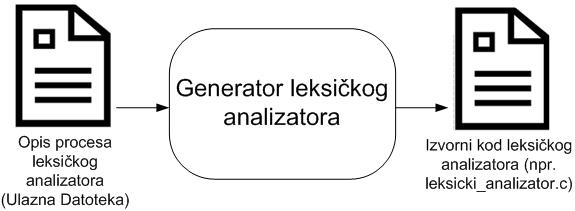
\includegraphics[width=0.7\textwidth]{slike/generator-leksickog-analizatora.jpg}
\caption{Način rada generatora leksičkog analizatora.}
\label{fig:generator-leksickog-analizatora}
\end{figure}

Način rada generatora leksičkog analizatora prikazan je slikom \ref{fig:generator-leksickog-analizatora}.
Generator leksičkog analizatora na standardnom ulazu dobiva opis procesa leksičkog analizatora.
Opis procesa leksičkog analizatora zadan je tekstualnom datotekom (dalje Ulazna Datoteka)\footnote{U skladu s napomenama u uvodu, ostvareni generator leksičkog analizatora treba čitati opis procesa leksičkog analizatora sa standardnog ulaza, a Ulazna Datoteka se onda preusmjerava na standardni ulaz prilikom pokretanja generatora.}.
Izlaz iz generatora leksičkog analizatora treba biti izvorni kod leksičkog analizatora napisan u jeziku izgradnje.
Ulazna Datoteka bit će zadana u sljedećem formatu:
\begin{description}
\itemsep 1pt
\item \emph{regularne definicije}
\item \%X \emph{stanja leksičkog analizatora}
\item \%L \emph{imena leksičkih jedinki}
\item \emph{pravila leksičkog analizatora}
\end{description}
U nastavku je objašnjeno kako pojedini dio datoteke izgleda.

\subsection{Regularne definicije}
Regularne definicije čine nadgradnju nad regularnim izrazima sa ciljem jednostavnijeg i preglednijeg opisa nekog regularnog jezika.
Regularne definicije opisane su u udžbeniku predmeta “Uvod u teoriju računarstva” \cite[poglavlje 2.3.2]{utr}.
U nastavku su opisani regularni izrazi i oblik regularnih definicija koje će se koristiti u Ulaznoj Datoteci.

\subsubsection*{Oblik regularnih izraza}
Kako bi se pojednostavio postupak pretvorbe regularnih izraza koji se koriste za definiciju leksičkih jedinki u konačni automat, svi regularni izrazi u Ulaznoj Datoteci koristit će isključivo:
\begin{itemize}
\itemsep 1pt
\item izbor podizraza koristeći operator \verb=|=
\item nadovezivanje (slijedno napisani znakovi ili grupe znakova, bez posebnog operatora)
\item Kleeneov operator ponavljanja \verb=*= (ponavljanje nula ili više puta)
\item grupiranje koristeći oble zagrade \verb=(= i \verb=)=
\end{itemize}

Kao što je uobičajeno, prednost operatora ponavljanja \verb=*= veća je od prednosti nadovezivanja, a prednost nadovezivanja veća je od prednosti operatora izbora \verb=|=.
Odgovarajuća interpretacija regularnog izraza koja nije u skladu s ovim prednostima, može se postići grupiranjem koristeći zagrade.

Dodatno, zbog jednostavnosti, za prazan niz \(\varepsilon\) će se koristiti znak \verb=$= (dolar).
Zbog toga nigdje u regularnom izrazu neće biti praznih podizraza (npr. \verb=a||b= će biti zapisano kao \verb=a|$|b=).
U izrazima se neće pojaviti uzastopni operatori ponavljanja (na primjer \verb=a**=).

\subsubsection*{Regularne definicije u Ulaznoj Datoteci}
U Ulaznoj Datoteci bit će jedna regularna definicija po retku, sljedećeg oblika:\\
\verb|{|\emph{imeRegularneDefinicije}\verb|}|\textvisiblespace\emph{regularniIzraz}

Pritom, \emph{imeRegularneDefinicije} može sadržavati mala i velika slova engleske abecede, a \emph{regularniIzraz} je regularni izraz oblika u skladu s prije opisanim pravilima pri čemu osim pojedinačnih znakova smije sadržavati i proizvoljan broj referenci na prethodno definirane regularne definicije (vidi primjer ispod).
Početni znak \verb|{| će se nalaziti u prvom stupcu određenog retka, a između znaka \verb|}| i početka regularnog izraza nalazit će se točno jedan razmak.
U području regularnih definicija u Ulaznoj Datoteci neće se nalaziti niti jedan prazan redak.

Na primjer, dio regularnih definicija u Ulaznoj Datoteci može izgledati ovako:

\begin{lstlisting}[caption={Primjer regularnih definicija u Ulaznoj Datoteci.},label=lst:regdef]
{oktalnaZnamenka} 0|1|2|3|4|5|6|7
{dekadskaZnamenka} {oktalnaZnamenka}|8|9
{hexZnamenka} a|b|c|d|e|f|{dekadskaZnamenka}|A|B|C|D|E|F
\end{lstlisting}

Kao što se vidi u zadnjem retku primjera u ispisu \ref{lst:regdef}, referenca na prethodno definiranu regularnu definiciju može se nalaziti bilo gdje u regularnom izrazu.

\subsection{Stanja leksičkog analizatora}
Za pojedine klase leksičkih jedinki nužno je promatrati lijevi kontekst, tj.~dio ulaznog niza koji je pročitan prije podniza koji čini leksičku jedinku.
Jedan od načina praćenja lijevog konteksta koji se često koristi u leksičkim analizatorima su stanja leksičkog analizatora.

Za potrebe generatora leksičkog analizatora koji se gradi u sklopu prve laboratorijske vježbe, u Ulaznoj Datoteci će nakon zadnje regularne definicije biti redak u kojem su definirana stanja koja će koristiti leksički analizator.
Redak će započeti znakovima \verb=%X= i točno jednim razmakom, nakon kojeg slijedi niz jedne ili više oznaka stanja odvojenih točno jednim razmakom (vidi primjer ispod).
Oznake stanja će se sastojati od malih i velikih slova engleske abecede i započinjat će nizom \verb=S_= (to će ujedno biti jedino mjesto u imenu stanja na kojem će biti znak \verb=_= (engl. \emph{underscore})).
Prvo stanje navedeno nakon \verb=%X= je početno stanje leksičkog analizatora.
Na primjer, definicija stanja leksičkog analizatora može izgledati kao u ispisu \ref{lst:stanja}.

\begin{lstlisting}[caption={Primjer imena stanja u Ulaznoj Datoteci.},label=lst:stanja]
%X S_pocetno S_komentar S_unarniMinus
\end{lstlisting}

\subsection{Imena leksičkih jedinki}
Odmah u sljedećem retku nakon definicije stanja leksičkog analizatora, u Ulaznoj Datoteci nalazit će se redak koji definira imena leksičkih jedinki koje generirani leksički analizator treba koristiti.
Redak će započeti znakovima \verb=%L= i točno jednim razmakom, nakon kojeg slijedi niz jednog ili više imena leksičkih jedinki odvojenih točno jednim razmakom (vidi primjer ispod).
Imena leksičkih jedinki će se sastojati od malih i velikih slova engleske abecede i znakova \verb=_= (engl. \emph{underscore}).
Na primjer, definicija imena leksičkih jedinki može izgledati kao u ispisu \ref{lst:imena_jedinki}.

\begin{lstlisting}[caption={Primjer imena stanja u Ulaznoj Datoteci.},label=lst:imena_jedinki]
%L IDENTIFIKATOR brojcanaKonstanta znakovnaKonstanta OP_PLUS
\end{lstlisting}

\subsection{Pravila leksičkog analizatora}
Pravila leksičkog analizatora definiraju sve leksičke jedinke ulaznog jezika i definiraju na koji način će generirani leksički analizator pohraniti sve potrebne podatke vezane uz leksičku jedinku.
U Ulaznoj Datoteci će pravila leksičkog analizatora biti navedena nakon retka koji definira imena leksičkih jedinki u sljedećem obliku:\\
\verb=<=\emph{imeStanja}\verb=>=\emph{regularniIzraz}\\
\verb|{|\\
\emph{argumentiAkcije}\\
\verb|}|

U datoteci će biti proizvoljan broj pravila, jedno iza drugog bez praznih redaka između pravila.
\emph{imeStanja} odgovarat će nekom od stanja definiranih ranije i bit će okruženo znakovima \verb|<| i \verb|>|.
\emph{regularniIzraz} slijedit će neposredno nakon znaka \verb|>| (bez razmaka) i bit će u prethodno opisanom formatu.
U regularnom izrazu mogu se pojaviti imena definirana u regularnim definicijama okružena znakovima \verb|{| i \verb|}| (vidi primjer ispod).

\emph{Napomena: Sva pravila} leksičkog analizatora imat će zadano stanje na početku pravila.
Određeno pravilo je aktivno ako i samo ako se leksički analizator nalazi u odgovarajućem stanju (vidi savjete za implementaciju ispod).
Prvenstveni razlog za ovakvu definiciju pravila je uniformnost što omogućuje jednostavniju implementaciju.

U sljedećem retku definicije pravila nalazit će se znak \verb|{| koji započinje dio za definiciju argumenata akcije.
Svi retci argumenata akcije počet će u prvom stupcu i niti jedan neće započinjati znakom \verb|}|.
Završetak dijela argumenata akcije bit će jednoznačno određen retkom koji sadrži samo znak \verb|}|.
Argumenti akcije određuju što generirani leksički analizator treba učiniti kada prepozna odgovarajuću leksičku jedinku.
Svaka akcija imat će jedan do četiri argumenata, svaki u svom retku.
U prvom retku argumenata akcije uvijek će se nalaziti ime pripadne leksičke jedinke (jedno od imena definiranih ranije u Ulaznoj Datoteci) ili znak \(-\) (minus).
U slučaju da je u akciji navedeno ime leksičke jedinke, generirani leksički analizator treba zadanu leksičku jedinku dodati u odgovarajuće tablice i u tablice upisati početne vrijednosti za tu leksičku jedinku (ovo je detaljnije objašnjeno u poglavlju \ref{sec:leksicki_analizator} ove upute).
S druge strane, znak minus označava da pročitani dio ulaznog niza treba odbaciti i da ne predstavlja leksičku jedinku.
Odbacivanje će se koristiti za izbacivanje komentara, bjelina i slično.
Pojedine akcije imat će jedan do tri posebna argumenta koji redom omogućuju brojanje redaka, upravljanje stanjem leksičkog analizatora i razrješavanje nejednoznačnosti.

Prvi posebni argument je \verb|NOVI_REDAK| što označava leksičkom analizatoru da je u izvornoj datoteci programa koji se prevodi došlo do promjene retka.
Retci se broje kako bi jezični procesor mogao ispisivati korisne podatke o mjestu pogreške, i tijekom leksičke analize i tijekom ostalih faza rada.
Povećani broj retka odnosi se tek na sljedeću leksičku jedinku, tj.~ako akcija prepoznaje neku leksičku jedinku (u prvom retku argumenata akcije nalazi se neko ime leksičke jedinke, a ne znak \(-\)) i ima argument \verb|NOVI_REDAK|, za broj retka te leksičke jedinke zapisuje se stari broj retka, prije uvećanja.

Drugi posebni argument je \verb|UDJI_U_STANJE| \emph{imeStanja} kojim leksički analizator prelazi iz trenutnog stanja u stanje \emph{imeStanja}.
Niz znakova \emph{imeStanja} bit će odvojen od niza \verb|UDJI_U_STANJE| točno jednim razmakom.
Treći posebni argument je \verb|VRATI_SE| \emph{naZnak} koji određuje da se od pročitanih znakova u leksičku jedinku treba grupirati prvih \emph{naZnak} znakova, a ostali znakovi vraćaju se u ulazni niz, kao da nisu ni pročitani (vidi primjer).
Ova naredba je ekvivalentna naredbi \verb|yyless(naZnak)| u Lexu.
\emph{naZnak} će biti cijeli broj bez vodećih nula i bit će odvojen od niza \verb|VRATI_SE| točno jednim razmakom.
Svi posebni argumenti prikazani su u primjeru, uz dodatne komentare u savjetima za implementaciju.

\subsection{Specijalni znakovi}\label{sec:specijalni_znakovi}
Pojedini znakovi se u opisu regularnih definicija i regularnih izraza u pravilima leksičkog analizatora koriste kao posebne oznake.
Kako bi generirani leksički analizator mogao te iste znakove prepoznati u izvornom kodu programa koji se prevodi, nužno je uvesti sustav prefiksiranja (engl. \emph{escaping}).
Kao što je uobičajeno, specijalni znakovi prefiksiraju se znakom \verb|\| (engl. \emph{backslash}) da bi dobili svoje izvorno značenje.
Dodatno, kako bi se u regularnom izrazu mogao prepoznati i sam znak \verb|\|, on se također mora prefiksirati dodatnim znakom \verb|\| (vidi primjer ispod).
Specijalni znakovi koji se koriste u generatoru leksičkog analizatora su:\\
\verb=( ) { } | * $ \=

Osim ovih znakova, generator leksičkog analizatora mora u Ulaznoj Datoteci prepoznati i niz znakova \verb|\n| kao znak za novi redak i niz znakova \verb|\t| kao znak tab.
Dodatno, razmak ćemo označavati nizom \verb|\_| (\emph{backslash underscore}) kako bi Ulazna Datoteka bila čitljivija i kako ne bi bilo problema s uređivačima teksta koji brišu razmake na krajevima redaka.

\subsection{Primjer}\label{sec:generator_primjer}
U primjeru je prikazana Ulazna Datoteka jednostavanog jezika za računanje matematičkih izraza.
Jezik podržava samo binarno oduzimanje i unarni minus pa ćemo ga zvati \emph{minusLang}.
Unarni minus može se pojaviti više puta uzastopce.
Podržani su samo cijeli brojevi u dekadskom, oktalnom ili heksadekadskom zapisu.
Grupiranje se ostvaruje korištenjem oblih zagrada.
Dozvoljen je slobodan način zapisa matematičkog izraza kroz više redaka i s proizvoljnim brojem praznina.
Također su dozvoljeni i komentari koji prolaze kroz proizvoljan broj redaka, a ograđeni su nizovima \verb=#|= i \verb=|#=.
Zbog jednostavnosti Ulazne Datoteke, u jeziku nije dozvoljeno da se komentar pojavi ispred unarnog minusa.

Primjer programa pisanog u zadanom jeziku prikazan je u ispisu \ref{lst:minusLang_primjer}.
Ulazna Datoteka za leksičku analizu ovog jezika mogla bi izgledati \href{https://github.com/fer-ppj/ppj-labosi/raw/master/res/lab1/minusLang.lan}{ovako}.

\begin{lstlisting}[caption={Primjer programa pisanog u jeziku \emph{minusLang}.},label=lst:minusLang_primjer]
#| ovo je primjer |#
3 -  -0x12 - ( #| ovdje ce doci grupirane
		operacije |#
3- -
--076) #| 3 - ---076 = 3 - -076 = 3 + 076 |#

\end{lstlisting}

U području regularnih definicija, definirana je jedinstvena definicija broja koja prihvaća zapis broja u sve tri baze (oktalne brojeve ne trebamo posebno definirati jer izgledaju kao dekadski s vodećom nulom).
To znači da leksička analiza neće razlikovati brojevne baze, odnosno neće provjeravati sadrži li oktalni broj znamenke \verb|8| ili \verb|9|, nego će te provjere odraditi neka kasnija faza rada jezičnog procesora, tipično semantička analiza\footnote{O ovom i sličnim pitanjima bit će govora na predavanjima predmeta tijekom semestra.}.

Na početku regularnog izraza definicije \verb|{sviZnakovi}| nalaze se svi specijalni znakovi, prefiksirani znakom \verb|\|, kao što je ranije opisano.
Izbacivanje komentara odrađuje se s četiri pravila prikazana u ispisu \ref{lst:minusLang_komentari}.

\begin{lstlisting}[caption={Pravila za izbacivanje komentara iz ulaznog programa.},label=lst:minusLang_komentari]
<S_pocetno>#\|
{
-
UDJI_U_STANJE S_komentar
}
<S_komentar>\|#
{
-
UDJI_U_STANJE S_pocetno
}
<S_komentar>\n
{
-
NOVI_REDAK
}
<S_komentar>{sviZnakovi}
{
-
}
\end{lstlisting}

Prva akcija prepoznaje početni niz znakova koji označava komentar.
Za prepoznavanje specijalnog znaka \verb=|= koristi se prefiks \verb|\|.
Slično, drugo pravilo pronalazi kraj komentara i vraća leksički analizator u početno stanje.
S obzirom na to da se komentari mogu provlačiti kroz proizvoljan broj redaka, nužno je i unutar stanja za prepoznavanje komentara nastaviti brojati retke.
Brojanje redaka ostvaruje trećim pravilom.
Konačno, u komentaru se može pojaviti mnogo znakova koji inače nisu dozvoljeni van komentara.
Važno je primijetiti da četvrto pravilo prepoznaje jedan po jedan znak unutar komentara koristeći regularnu definiciju \verb|{sviZnakovi}|.
Na taj način će biti moguće prepoznati niz znakova koji predstavlja kraj komentara (prioritet po duljini, a i po redoslijedu pravila) i znak kraja retka (prioritet po redoslijedu pravila).
Naime, i znak novog retka i oba znaka koji predstavljaju kraj komentara nalaze se u regularnom izrazu za definiciju \verb|{sviZnakovi}|.
Kada bi se za četvrto pravilo koristio složeniji regularni izraz, na primjer \verb|{sviZnakovi}{sviZnakovi}*| s ciljem prepoznavanja cijelog komentara, onda bi cijeli program nakon prvog početka komentara bio preskočen zbog pririteta po duljini (osim ako komentar sadrži nula znakova).

Prepoznavanje unarnog minusa riješeno je većim dijelom kroz pravila prikazana u ispisu \ref{lst:minusLang_unarni_minus}.

\begin{lstlisting}[caption={Pravila za detekciju unarnog minusa.},label=lst:minusLang_unarni_minus]
<S_pocetno>-{bjelina}*-
{
OP_MINUS
UDJI_U_STANJE S_unarni
VRATI_SE 1
}
<S_pocetno>\({bjelina}*-
{
LIJEVA_ZAGRADA
UDJI_U_STANJE S_unarni
VRATI_SE 1
}
<S_unarni>-
{
UMINUS
UDJI_U_STANJE S_pocetno
}
\end{lstlisting}

U prva dva pravila definirana su dva mjesta gdje se unarni minus može pojaviti --- iza binarnog operatora oduzimanja ili iza otvorene zagrade.
Između lijevog i desnog znaka može se pojaviti proizvoljan broj bjelina.
U oba pravila koristi se posebni argument \verb|VRATI_SE| \emph{naZnak}.
Na primjer, ako leksički analizator u stanju \verb|S_pocetno| pročita niz\\
\verb|-\t\t \n -|\\
tada akcija prvog pravila treba prepoznati \emph{samo prvi minus} kao jedinku \verb|OP_MINUS| (zbog \verb|VRATI_SE 1|, što znači da se "glava za čitanje" treba vratiti na znak s indeksom \verb|1| u pročitanom nizu, pri čemu indeksi počinju od \verb|0|).
Dodatno, leksički analizator treba ući u stanje \verb|S_unarni| i vratiti sve znakove osim prvog minusa u ulazni niz (vidi savjete za implementaciju).
Bitno je primijetiti da je vraćanje znakova u ulazni niz ključan element ove akcije.
Na taj način će pravilo za brojanje redaka u stanju \verb|S_unarni| dobiti pročitani znak kraja retka i brojanje redaka će raditi ispravno.

S obzirom na to da je u definiciji jezika navedeno da se unarni minus može pojavljivati više puta uzastopce, nužno je uvesti i dodatno pravilo (zadnje pravilo u datoteci) koje je prikazano u ispisu \ref{lst:minusLang_unarni_minus_ponavljanje}.

\begin{lstlisting}[caption={Pravila za detekciju ponavljanja unarnog minusa.},label=lst:minusLang_unarni_minus_ponavljanje]
<S_unarni>-{bjelina}*-
{
UMINUS
VRATI_SE 1
}
\end{lstlisting}

\section{Leksički analizator}\label{sec:leksicki_analizator}
Izlaz iz generatora leksičkog analizatora treba biti izvorni kod leksičkog analizatora pisan u jeziku izgradnje jezičnog procesora.
Dio koda leksičkog analizatora, primjerice deklaracije tipova podataka, uključivanje biblioteka te algoritam leksičkog analizatora, potpuno je neovisno o Ulaznoj Datoteci.
Na osnovi Ulazne Datoteke potrebno je generirati tablicu konačnog automata koju će leksički analizator koristiti u algoritmu grupiranja znakova u leksičke jedinke.
Način konstruiranja konačnog automata (\(\varepsilon\)-NKA) iz regularnog izraza opisan je u \cite[poglavlje 2.2.2]{utr}, a pomoć za implementaciju tog algoritma navedena je u savjetima za implementaciju u ovom dokumentu.

\begin{figure}[htb!]
\centering
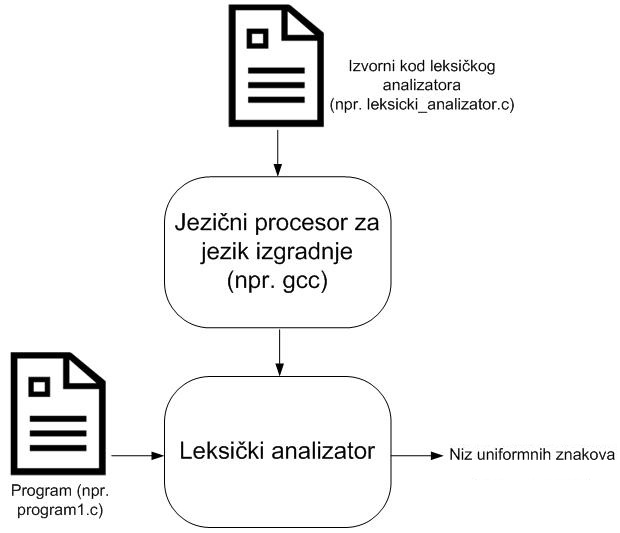
\includegraphics[width=0.7\textwidth]{slike/leksicki-analizator.jpg}
\caption{Način rada leksičkog analizatora.}
\label{fig:leksicki-analizator}
\end{figure}

Slika \ref{fig:leksicki-analizator} prikazuje dinamiku rada leksičkog analizatora.
Izvorni kod leksičkog analizatora dobiven primjenom izgrađenog generatora leksičkog analizatora treba prevesti u izvodivi oblik primjenom odgovarajućeg jezičnog procesora (ako je jezik izgradnje interpretirani jezik onda se ovaj korak preskače).
Izvodivi leksički analizator čita izvorni kod nekog programa pisanog u zadanom izvornom jeziku (na primjer jeziku \emph{C}) \emph{sa standardnog ulaza}.
Rezultat izvođenja leksičkog analizatora u jezičnom procesoru su \emph{niz uniformnih znakova} i \emph{tablica znakova}.

\subsection{Ispis leksičkog analizatora}
Za potrebe prve laboratorijske vježbe, leksički analizator \emph{na standardni izlaz} treba za svaki element niza uniformnih znakova ispisati redak sljedećeg oblika:\\
\\
\emph{uniformniZnak}\textvisiblespace\emph{redakPrograma}\textvisiblespace\emph{leksičkaJedinka}\\
\\
Pritom je \emph{uniformniZnak} odgovarajući uniformni znak iz Ulazne datoteke, \emph{redakPrograma} broj retka u ulaznom programu u kojem se leksička jedinka nalazi ako se \textbf{retci broje od 1} i \emph{leksičkaJedinka} je niz znakova ulaznog programa koji su grupirani u leksičku jedinku.
Ta tri dijela retka međusobno su odvojeni sa po jednim razmakom.
Primjer izlaza prikazan je u poglavlju \ref{sec:leksicki_analizator_primjer}.

\subsection{Strukture podataka leksičkog analizatora}
Leksički analizator na ulazu prima programski kod u jeziku opisanom Ulaznom Datotekom.
Kao rezultat, leksički analizator treba stvoriti niz uniformnih znakova i tablicu znakova (engl. \emph{symbol table}).
Zbog jednostavnosti Ulazne Datoteke, tablica znakova može biti jedino homogena, odnosno jedna tablica (kako god bila implementirana) sadržavat će na kraju rada leksičkog analizatora sve leksičke jedinke koje se nalaze u ulaznom programu.
Drugim rječima, Ulazna Datoteka ne omogućuje razvrstavanje simbola u tablicu ključnih riječi, tablicu konstanti i tablicu identifikatora.

Niz uniformnih znakova mora za svaku prepoznatu leksičku jedinku sadržavati ime leksičke jedinke, redak u kojem se ta jedinka nalazi u ulaznom programu i neku informaciju kako doći do odgovarajućeg zapisa u tablici znakova; to može biti pokazivač, indeks ili nešto treće.

Nakon završetka rada leksičkog analizatora, tablica znakova treba sadržavati točno jedan zapis za svaku leksičku jedinku u ulaznom programu.

\subsection{Algoritam leksičkog analizatora}
U udžbeniku su opisana dva algoritma leksičkog analizatora.
U poglavlju 2.9.6, opisan je algoritam zasnovan na DKA, a u poglavlju 2.9.7 algoritam zasnovan na \(\varepsilon\)-NKA.
Implementacijom algoritma zasnovanog na \(\varepsilon\)-NKA neće biti potrebno ostvarivati pretvorbu \(\varepsilon\)-NKA u DKA (koja je obrađena na predmetu “Uvod u teoriju računarstva”) te je stoga taj algoritam predložen za prvu laboratorijsku vježbu (vidi savjete za implementaciju).

\subsection{Razrješavanje nejednoznačnosti}
Generirani leksički analizator nejednoznačnost treba rješavati koristeći pravila P2 i P3 iz poglavlja 2.9.3 i 2.9.4 udžbenika (prioritet po duljini prepoznatog niza i prioritet po poretku pravila).

\subsection{Postupak oporavka od pogreške}
Za postupak oporavka od pogreše treba koristiti jednostavan postupak odbacivanja prvog znaka iz ulaznog programa kao što je opisano u poglavlju 2.9.5 udžbenika.
Prijavu pogrešaka obavljati isključivo na izlaz za greške (\emph{stderr}).
Dodatno, iako se u ispisu leksičkog analizatora eksplicitno ne navode greške niti nije vidljivo kako se analizator oporavlja od pogreške, ispravnost implementacije ovog postupka utjecat će na ispis za sve ulazne programe koji sadrže barem jednu leksičku pogrešku.

\subsection{Primjer}\label{sec:leksicki_analizator_primjer}
Kao nastavak prije obrađenog primjera, prikazat ćemo rezultat rada leksičkog analizatora generiranog za primjer u poglavlju \ref{sec:generator_primjer} ovih uputa, nad ulaznim programom koji je zbog preglednosti ponovljen u ispisu \ref{lst:minusLang_primjer_ponovljen}.

\begin{lstlisting}[caption={Primjer programa pisanog u jeziku \emph{minusLang}.},label=lst:minusLang_primjer_ponovljen]
#| ovo je primjer |#
3 -  -0x12 - ( #| ovdje ce doci grupirane
		operacije |#
3- -
--076) #| 3 - ---076 = 3 - -076 = 3 + 076 |#

\end{lstlisting}

Datoteka s ovim primjerom za potrebe testiranja može se pronaći \href{https://github.com/fer-ppj/ppj-labosi/raw/master/res/lab1/primjer.minus}{ovdje}.
Leksički analizator u skladu s ranije opisanom Ulaznom Datotekom generira sljedeći niz uniformnih znakova i tablicu znakova:

\begin{table}[ht]
\begin{minipage}[b]{0.5\linewidth}
\centering
\begin{tabular}{|l|c|c|}
\hline
uniformni znak&redak&indeks\\
\hline
OPERAND&2&0\\
\hline
OP\_MINUS&2&1\\
\hline
UMINUS&2&2\\
\hline
OPERAND&2&3\\
\hline
OP\_MINUS&2&1\\
\hline
LIJEVA\_ZAGRADA&2&4\\
\hline
OPERAND&4&0\\
\hline
OP\_MINUS&4&1\\
\hline
UMINUS&4&2\\
\hline
UMINUS&5&2\\
\hline
UMINUS&5&2\\
\hline
OPERAND&5&5\\
\hline
DESNA\_ZAGRADA&5&6\\
\hline
\end{tabular}
\end{minipage}
\hspace{0.5cm}
\begin{minipage}[b]{0.5\linewidth}
\centering
\begin{tabular}{|l|l|l|}
\hline
0&OPERAND&3\\
\hline
1&OP\_MINUS&-\\
\hline
2&UMINUS&-\\
\hline
3&OPERAND&0x12\\
\hline
4&LIJEVA\_ZAGRADA&(\\
\hline
5&OPERAND&076\\
\hline
6&DESNA\_ZAGRADA&)\\
\hline
\end{tabular}
\end{minipage}
\end{table}

U drugom stupcu niza uniformnih znakova naveden je redak u kojem se uniformni znak nalazi u ulaznoj datoteci.
U trećem stupcu naveden je indeks u tablicu znakova.

U ovom primjeru važno je uočiti dvije stvari.
Prvo, iako se operand \verb|3| u tekstu programa pojavljuje na dva mjesta, u tablici postoji samo jedan (zajednički) zapis jer se radi o dva pojavljivanja iste leksičke jedinke.
Drugo, iako se zapisi za binarni i unarni minus u tekstu programa ne razlikuju, u tablici znakova postoje zasebni zapisi za binarni i unarni minus zato jer se radi o različitim leksičkim jedinkama.

Očekivani ispis na standardni izlaz prikazan je \href{https://github.com/fer-ppj/ppj-labosi/raw/master/res/lab1/minus_primjer_izlaz.txt}{ovdje}.
Treba uočiti da ispis završava praznim retkom tj.~da svi retci (osim tog praznog) završavaju znakom kraja retka.

\section{Način računalnog ocjenjivanja rješenja}
Za potrebe računalnog ocjenjivanja rješenje prve laboratorijske vježbe treba predati u jednoj \emph{zip} datoteci.
U korijenskom direktoriju trebaju se nalaziti \textbf{sve} datoteke s izvornim kodom \textbf{generatora} leksičkog analizatora.
Korijenski direktorij \emph{zip} datoteke mora sadržavati poddirektorij \texttt{analizator}.
Poddirektorij \texttt{analizator} može inicijalno sadržavati dijelove implementacije leksičkog analizatora koji ne ovise o Ulaznoj datoteci, ali i ne mora sadržavati ništa.
Na primjer, za rješenje u jeziku \emph{C}, sadržaj \emph{zip} datoteke mogao bi izgledati kao u ispisu \ref{lst:gla_zip_struktura}.

\begin{lstlisting}[caption={Primjer sadržaja \emph{zip} datoteke. Imena datoteka \emph{nisu važna}.},label=lst:gla_zip_struktura]
analizator/bar.c
analizator/bar.h
analizator/lekser.h
analizator/predlozak.txt
foo.c
foo.h
generator.c
\end{lstlisting}

Za prevođene jezike izgradnje, sustav za računalno ocjenjivanje će prevesti predane datoteke u izvodivi oblik generatora leksičkog analizatora u korijenskom direktoriju.
Za prethodni primjer, rezultat bi mogao izgledati kao u ispisu \ref{lst:gla_preveden}.

\begin{lstlisting}[caption={Primjer sadržaja korijenskog direktorija nakon prevođenja generatora.},label=lst:gla_preveden]
analizator/bar.c
analizator/bar.h
analizator/lekser.h
analizator/predlozak.txt
foo.c
foo.h
generator.c
generator.exe
\end{lstlisting}

Generatoru leksičkog analizatora na standardni ulaz se predaje opis procesa leksičkog analizatora, a generator priprema izvorni kod leksičkog analizatora u poddirektoriju \texttt{analizator}, kao u ispisu \ref{lst:la_pripremljen}.
Važno je uočiti da se \emph{izlaz generatora} ne provjerava izravno --- generator ne mora ispisati ništa, ali mora pripremiti tj.~generirati analizator.

\begin{lstlisting}[caption={Primjer sadržaja korijenskog direktorija nakon izvođenja generatora.},label=lst:la_pripremljen]
analizator/bar.c
analizator/bar.h
analizator/lekser.h
analizator/lekser.c
analizator/predlozak.txt
analizator/tablica.txt
foo.c
foo.h
generator.c
generator.exe
\end{lstlisting}

Nakon izvođenja generatora leksičkog analizatora, u poddirektoriju \texttt{analizator} mora se nalaziti sav potrebni izvorni kod za prevođenje leksičkog \textbf{analizatora}.
Sustav će prevesti datoteke u poddirektoriju u izvodivi oblik leksičkog analizatora u istom poddirektoriju, kao što je prikazano u ispisu \ref{lst:la_preveden}.

\begin{lstlisting}[caption={Primjer sadržaja korijenskog direktorija nakon izvođenja generatora.},label=lst:la_preveden]
analizator/analizator.exe
analizator/bar.c
analizator/bar.h
analizator/lekser.h
analizator/lekser.c
analizator/predlozak.txt
analizator/tablica.txt
foo.c
foo.h
generator.c
generator.exe
\end{lstlisting}

Konačno, izvodivi leksički analizator na standardni ulaz dobiva izvorni kod programa i treba ispisati rezultat izvođenja kao što je ranije opisano.

Uočite da su \textbf{generator} i \textbf{analizator} dva \emph{odvojena programa}.
Nije dozvoljeno kopirati Ulaznu datoteku u "generatoru" i onda ju ponovno parsirati u "analizatoru", stvarati automate i tek onda analizirati ulazni program.
Generator je taj program koji mora završiti definiciju analizatora.
To se, na primjer, može ostvariti tako da generator generira programski kod koji u analizatoru inicijalizira tablice automata ili da generira datoteku s tablicama automata koju onda analizator čita.

Za rješenja u \emph{Javi} i \emph{C\#}-u, ulazna točka u generator \textbf{mora biti} u razredu \texttt{GLA}, a ulazna točka u analizator u razredu \texttt{LA}.
Za rješenja u \emph{Pythonu}, za izvođenje generatora će se pozvati datoteka \texttt{GLA.py}, a za izvođenje analizatora datoteka \texttt{LA.py}.

Detalji oko predaje, kao što su inačice alata koji će se koristiti za prevođenje i izvođenje rješenja, bit će objavljeni naknadno na FERWebu.

\section{Savjeti za implementaciju}
Savjeti za implementaciju navedeni u ovom poglavlju zamišljeni su kao pomoć u izradi generatora leksičkog analizatora.
Kao takvi, nisu obvezujući i grupe po vlastitom nahođenju mogu dio ili sve savjete u ovom poglavlju zanemariti.

\subsection{Generiranje koda leksičkog analizatora}
Veliki dio izvornog koda generiranog leksičkog analizatora neovisan je od Ulazne Datoteke i treba biti napisan unaprijed.
Preporuča se da se taj dio koda zasebno razvije i testira, na primjer koristeći izmišljenu tablicu konačnog automata.
Na taj način, generator leksičkog analizatora može razvijeni kod iskopirati u datoteku s izvornim kodom leksičkog analizatora i dopuniti datoteku definicijom tablice konačnog automata i slično.

\subsection{Priprema regularnih izraza za generiranje konačnog automata}
Prije generiranja \(\varepsilon\)-NKA iz regularnog izraza, potrebno je sve regularne definicije koji se pojavljuju u regularnom izrazu zamijeniti odgovarajućim regularnim izrazima.
S obzirom na ograničenja regularnih definicija, svaka regularna definicija će prije njenog referenciranja biti definirana.
Prema tome, zamjena regularnih definicija se tijekom rada generatora leksičkog analizatora može obaviti algoritmom prikazanim u pseudokodu u ispisu \ref{lst:priprema_regexa}.

\begin{lstlisting}[caption={Pseudokod za pripremu regularnih izraza za generiranje konačnog automata.},label=lst:priprema_regexa]
za svaku regularnu definiciju {regDef} u Ulaznoj Datoteci
	neka je regEx regularni izraz koji opisuje definicjiu {regDef}
	za svaku referencu {refRegDef} u regularnom izrazu regEx
		zamijeni {refRegDef} u izrazu regEx s
           "(" + regularniIzraz[{refRegDef}] + ")"
	regularniIzraz[{regDef}] = regEx
\end{lstlisting}

Ključno je primijetiti da se koristeći ovaj algoritam svakoj regularnoj definiciji neposredno nakon što je pročitana iz Ulazne Datoteke pridruži "čisti" regularni izraz koji ne referencira niti jednu regularnu definiciju.
Također, kako bi se očuvala očekivana prednost operatora, nužno je prije zamjene regularni izraz koji opisuje neku regularnu definiciju okružiti zagradama.
Koristeći vrlo sličan algoritam i "čiste" regularne izraze za regularne definicije, moguće je pripremiti sve regularne izraze iz Ulazne Datoteke za generiranje konačnog automata, tj.~zamijeniti sve reference na regularne definicije odgovarajućim regularnim izrazom.

Na primjer, neka su zadane sljedeće regularne definicije:\\
\verb={znamenka} 0|1|2|3|4|5|6|7|8|9=\\
\verb={hexZnamenka} {znamenka}|a|b|c|d|e|f|A|B|C|D|E|F=

Regularni izraz za regularnu definiciju \verb|{znamenka}| ne sadrži reference na niti jednu regularnu definiciju.
Regularni izraz za definiciju \verb|{hexZnamenka}| sadrži referencu na definiciju \verb|{znamenka}| tako da će primjenom opisanog algoritma regularni izraz za definiciju \verb|{hexZnamenka}| biti preveden u \verb=(0|1|2|3|4|5|6|7|8|9)|a|b|c|d|e|f|A|B|C|D|E|F=

Kada bi u dijelu pravila bilo definirano pravilo:\\
\verb=<S_nekoStanje>0x{hexZnamenka}{hexZnamenka}*=\\
\verb={=\\
\verb=HEX_KONSTANTA=\\
\verb=}=\\
uvrštavanjem takvog regularnog izraza za definiciju \verb|{hexZnamenka}| dobili bi jednostavan regularan izraz za prikazano pravilo (oba retka dio su istog izraza):\\
\verb=0x((0|1|2|3|4|5|6|7|8|9)|a|b|c|d|e|f|A|B|C|D|E|F)=\\
\verb=((0|1|2|3|4|5|6|7|8|9)|a|b|c|d|e|f|A|B|C|D|E|F)*=

Ovakav regularni izraz može se prevesti u \(\varepsilon\)-NKA koristeći ranije spomenuti algoritam opisan u udžbeniku "Uvod u teoriju računarstva" \cite[poglavlje 2.2.2]{utr}.

\subsection{Izgradnja $\varepsilon$-NKA iz regularnih izraza za potrebe leksičkog analizatora}
Ako se u obradi referenci na regularne definicije koristi algoritam koji je opisan u prethodnom poglavlju, za regularne izraze definicija nije potrebno graditi konačne automate jer se ti regularni izrazi na tekstualnoj razini umeću u regularne izraze pravila.

Kao što je navedeno u opisu pravila, svako pravilo bit će pridruženo točno jednom stanju leksičkog analizatora.
Implementacija generatora mora osigurati da generirani leksički analizator koristi isključivo ona pravila koja su aktivna u trenutnom stanju leksičkog analizatora.
To ograničenje moguće je ostvariti tako da se za svako stanje leksičkog analizatora generira zaseban \(\varepsilon\)-NKA te se ulazni znakovi predaju samo automatu koji je zadužen za obradu trenutno aktivnog stanja leksičkog analizatora.

Postupak izgradnje \(\varepsilon\)-NKA za potrebe leksičkog analizatora opisan je u udžbeniku \cite[poglavlje 2.9.2]{udzbenik}.
Bitno je primijetiti da je prilikom dodavanja početnog stanja \(p_0\) (vidi udžbenik) i spajanja svih automata \(M_i\) u jedinstveni automat nužno osigurati da sva stanja u automatima \(M_i\) imaju jedinstvene oznake.
U suprotnom automat vrlo vjerojatno neće raditi ispravno!
Kako bi se izbjegla potreba za preimenovanjem stanja, moguće je umjesto spajanja automata \(M_i\) u jedinstveni automat za neko stanje leksičkog analizatora automate \(M_i\) pohraniti odvojeno.
Na taj način će svako pravilo pridruženo nekom stanju leksičkog analizatora imati svoj \(\varepsilon\)-NKA.
Ova promjena utječe na sam algoritam rada leksičkog analizatora opisan u \cite[poglavlje 2.9.7]{udzbenik} jer će leksički analizator umjesto jednog koristiti nekoliko \(\varepsilon\)-NKA.

Izgradnja \(\varepsilon\)-NKA za regularni izraz svakog pravila načelno je opisana u udžbeniku predmeta "Uvod u teoriju računarstva".
S obzirom na to da je postupak relativno složen, a nije središnja tema ove laboratorijske vježbe, u nastavku je dan pseudokod koji opisuje jedan način na koji se pretvorba može ostvariti.

Funkciji u pseudokodu predaje se regularni izraz i automat koji treba izgraditi.
Vizualno, automat se gradi s lijeva na desno pa se imena varijabli naslanjaju na tu predodžbu.
Funkcija kao rezultat vraća "lijevo" i "desno" stanje automata.
Lijevo stanje za cijeli izraz odgovara početnom stanju automata, a desno stanje za cijeli izraz odgovara prihvatljivom stanju automata.
Algoritam izgradnje \(\varepsilon\)-NKA iz regularnog izraza jamči da će automat imati točno jedno prihvatljivo stanje.
Poziv algoritma prikazan je u ispisu \ref{lst:regex_pseudo_poziv}.

\begin{lstlisting}[caption={Poziv funkcije \texttt{pretvori}.},label=lst:regex_pseudo_poziv]
ParStanja rezultat = pretvori(regularni_izraz, automat)
automat.pocetno_stanje = rezultat.lijevo_stanje
automat.prihvatljivo_stanje = rezultat.desno_stanje
\end{lstlisting}

Stanja automata označavat će se cijelim brojevima od nula na više.
Za dodavanje stanja automatu koristit će se funkcija \verb|novo_stanje|.
Funkcija \verb|novo_stanje| vraća oznaku dodanog stanja.
Pretpostavlja se da će početni broj stanja automata biti nula.
Pseudokod funkcije \verb|novo_stanje| prikazan je u ispisu \ref{lst:regex_pseudo_novo_stanje}.

\begin{lstlisting}[caption={Pseudokod funkcije za dodavanje stanja automatu.},label=lst:regex_pseudo_novo_stanje]
int novo_stanje(automat)
	automat.br_stanja = automat.br_stanja + 1
	vrati automat.br_stanja - 1
\end{lstlisting}

Prvi korak algoritma je potraga za operatorima izbora koji se nalaze izvan svih zagrada.
Operator izbora ima najnižu pretpostavljenu prednost od svih operatora koje koristimo u regularnim izrazima pa je zbog toga nužno kao prvi korak niz podijeliti na podnizove između kojih se može birati.
Na primjer, u regularnom izrazu\\
\verb=(\)a|b)\|\(|x*|y*=\\
postoje dva operatora izbora izvan svih zagrada (neposredno ispred \verb|x| i neposredno ispred \verb|y|).
Rezultat prvog koraka algoritma bila bi tri nova regularna izraza\\
\verb=(\)a|b)\|\(=\\
\verb|x*|\\
\verb|y*|

Traženje operatora izbora izvan svih zagrada zahtijeva brojanje zagrada s lijeva na desno.
Brojač zagrada kreće od \verb|0|, povećava se za jedan za svaku otvorenu zagradu, a smanjuje za jedan za svaku zatvorenu zagradu.
Ako algoritam naiđe na operator izbora kada je brojač zagrada jednak nuli, preostali dio izraza podijeli oko operatora izbora i nastavi dalje prema desno.
Iz primjera je očito da pritom posebnu pažnju treba posvetiti zagradama i operatorima izbora koji su prefiksirani znakom \verb|\| i nemaju svoje originalno značenje.
Općenito, nužno je provjeriti nalazi li se ispred određenog operatora paran ili neparan broj znakova \verb|\|.
U algoritmu pretvorbe koristit će se pomoćna funkcija \verb|je_operator| koja za dani regularni izraz i indeks operatora provjerava ima li operator svoje značenje ili je prefiksiran neparnim brojem znakova \verb|\|.
Pseudokod funkcije \verb|je_operator| prikazan je u ispisu \ref{lst:regex_pseudo_je_operator}.

\begin{lstlisting}[caption={Pseudokod funkcije \texttt{je\_operator}.},label=lst:regex_pseudo_je_operator]
bool je_operator(izraz, i)
	int br = 0
	dok je i-1>=0 && izraz[i-1]=='\\' // jedan \, kao u C-u
	    br = br + 1
	    i = i - 1
	kraj dok
	vrati br%2 == 0
\end{lstlisting}

Dio funkcije \verb|pretvori| koji broji zagrade i dijeli izraz na podizraze odvojene operatorom izbora prikazan je u ispisu \ref{lst:regex_pseudo_pretvori_1}.

\begin{lstlisting}[caption={Početak funkcije \texttt{pretvori}.},label=lst:regex_pseudo_pretvori_1]
ParStanja pretvori(izraz, automat)
	niz izbori
	int br_zagrada = 0
	za (i=0; i<duljina(izraz); i=i+1)
	  ako je izraz[i]=='(' && je_operator(izraz, i)
	    br_zagrada = br_zagrada + 1
	  inace ako je izraz[i]==')' && je_operator(izraz, i)
	    br_zagrada = br_zagrada - 1
	  inace ako je br_zagrada==0 && izraz[i]=='|' && je_operator(izraz, i)
	    grupiraj lijevi negrupirani dio niza znakova izraz u niz izbori
	  kraj ako
	kraj za
	ako je pronadjen barem jedan operator izbora
	  grupiraj preostali negrupirani dio niza znakova izraz u niz izbori
	...
\end{lstlisting}

Nakon ovog odsječka, moguće je da je u nizu pronađen neki broj operatora izbora ili da se izraz na najvišoj razini (dakle, izvan svih zagrada) sastoji samo od podizraza povezanih nadovezivanjem.
Nastavak algoritma koji započinje izgradnja automata prikazan je u ispisu \ref{lst:regex_pseudo_pretvori_2}.

\begin{lstlisting}[caption={Nastavak funkcije \texttt{pretvori}.},label=lst:regex_pseudo_pretvori_2]
    ...
    int lijevo_stanje = novo_stanje(automat)
    int desno_stanje = novo_stanje(automat)
    ako je pronadjen barem jedan operator izbora
        za (i=0; i<br_elemenata(izbori); i=i+1)
          ParStanja privremeno = pretvori(izbori[i], automat)
          dodaj_epsilon_prijelaz(automat,
             lijevo_stanje,         
             privremeno.lijevo_stanje)
          dodaj_epsilon_prijelaz(automat,
                              privremeno.desno_stanje,
                              desno_stanje)
        kraj za
    inace
      ...
\end{lstlisting}

Kao što je prikazano odsječkom u ispisu \ref{lst:regex_pseudo_pretvori_2}, ako su u izrazu pronađeni podizrazi odvojeni operatorom izbora, svaki podizraz se rekurzivno obradi pozivom funkcije \verb|pretvori| i lijeva i desna stanja dobivena od rekurzivnog poziva povežu se epsilon prijelazima s lijevim i desnim stanjem za cijeli izraz.
Ovaj postupak je poopćenje točke \emph{p4} u \cite[poglavlje 2.2.2]{utr}.
U ispisu \ref{lst:regex_pseudo_pretvori_3} je opisana obrada drugog slučaja u kojem nisu pronađeni operatori izbora.

\begin{lstlisting}[caption={Obrada nadovezivanja u funkciji \texttt{pretvori}.},label=lst:regex_pseudo_pretvori_3]
      ... // nastavlja se inace iz proslog odsjecka
      bool prefiksirano = laz
      int trenutno_stanje = lijevo_stanje
      za (i=0; i<duljina(izraz); i=i+1)
        ako je prefiksirano istina
          *slucaj 1*
        inace
          *slucaj 2*
        kraj ako
      kraj za
      dodaj_epsilon_prijelaz(automat, trenutno_stanje, desno_stanje)
\end{lstlisting}

Varijabla \verb|prefiksirano| služi za prepoznavanje je li trenutni znak u izrazu prefiksiran znakom \verb|\|.
Varijabla \verb|trenutno_stanje| sadrži broj najdesnijeg stanja u postupku izgradnje automata.
Kao što je prije spomenuto, postupak kreće s lijeva na desno.
Na kraju obrade cijelog izraza (zadnja linija pseudokoda), najdesnije generirano stanje povezuje se epsilon prijelazom s desnim stanjem koje će se vratiti na kraju funkcije.
Pri obradi svakog znaka izraza postoje dva slučaja, ovisno o tome je li znak prefiksiran znakom \verb|\| ili nije.
Pseudokod za \emph{slučaj 1} prikazan je u ispisu \ref{lst:regex_pseudo_slucaj_1}.

\begin{lstlisting}[caption={Slučaj 1 u funkciji \texttt{pretvori}.},label=lst:regex_pseudo_slucaj_1]
// slucaj 1
prefiksirano = laz
char prijelazni_znak
ako je izraz[i] == 't'
  prijelazni_znak = '\t' // jedan znak, kao u C-u
inace ako je izraz[i] == 'n'
  prijelazni_znak = '\n' // jedan znak, kao u C-u
inace ako je izraz[i] == '_'
  prijelazni_znak = ' ' // obican razmak
inace
  prijelazni_znak = izraz[i]
kraj ako

int sljedece_stanje = novo_stanje(automat)
dodaj_prijelaz(automat, trenutno_stanje, sljedece_stanje, 
    prijelazni_znak)
*provjeri ponavljanje*
trenutno_stanje = sljedece_stanje
\end{lstlisting}

Odsječak za slučaj 1 prvo postavlja varijablu \verb|prefiksirano| u laž zato jer je prefiks iz prošlog znaka potrošen na znak koji se trenutno obrađuje.
Ograničenja na Ulaznu Datoteku osiguravaju da će u slučaju 1 \verb|izraz[i]| biti neki od specijalnih znakova opisanih u ovoj uputi u poglavlju \ref{sec:specijalni_znakovi}.
Posebnu pažnju treba posvetiti znakovima za tab, novi redak i prazninu.
Prijelazni znak u automatu treba biti onaj znak kojeg će leksički analizator pročitati u ulaznom programu.
Nakon što je određen prijelazni znak, automatu se dodaje novo stanje i odgovarajući prijelaz. 

Provjera za operator ponavljanja odvojena je jer će se ponoviti nekoliko puta u cijelom pseudokodu.
Ponavljanje se prevodi u automat slično kao u točki \emph{p6} u \cite[poglavlje 2.2.2]{utr}.
Pseudokod je prikazan u ispisu \ref{lst:regex_pseudo_ponavljanje}.

\begin{lstlisting}[caption={Obrada ponavljanja Kleeneovim operatorom.},label=lst:regex_pseudo_ponavljanje]
// provjeri ponavljanje
ako je i+1<duljina(izraz) && izraz[i+1]=='*'
  dodaj_epsilon_prijelaz(automat, trenutno_stanje, sljedece_stanje)
  dodaj_epsilon_prijelaz(automat, sljedece_stanje, trenutno_stanje)
  i = i+1
kraj ako
\end{lstlisting}

Nakon dodavanja epsilon prijelaza koji obrađuju ponavljanje, znak ponavljanja se preskače pomicanjem indeksa za jedan unaprijed.

Obrada slučaja 2 u kojem znak nije prefiksiran znakom \verb|\| prikazana je u ispisu \ref{lst:regex_pseudo_slucaj_2}.

\begin{lstlisting}[caption={Slučaj 2 u funkciji \texttt{pretvori}.},label=lst:regex_pseudo_slucaj_2]
// slucaj 2
ako je izraz[i] == '\\' // jedan znak \, kao u C-u
  prefiksirano = istina
  nastavi za petlju // continue u C-u
kraj ako
ako je izraz[i] != '('
  *slucaj 2a*
inace
  *slucaj 2b*
kraj ako
\end{lstlisting}

U slučaju 2, prvo se provjerava je li trenutni znak baš znak \verb|\|.
Ako je, postavlja se varijabla prefiksirano i prelazi se na sljedeći znak.
U suprotnom, provjerava se je li trenutni znak otvorena zagrada koja započinje neki podizraz.
Time se slučaj dijeli na dva podslučaja.
Ako trenutni znak nije otvorena zagrada onda se sigurno radi o nekom znaku kojeg treba nadovezati na dosad izgrađeni automat.
Pseudokod za ovaj slučaj prikazan je u ispisu \ref{lst:regex_pseudo_slucaj_2a}.

\begin{lstlisting}[caption={Slučaj 2a u funkciji \texttt{pretvori}.},label=lst:regex_pseudo_slucaj_2a]
// slucaj 2a
int sljedece_stanje = novo_stanje(automat)
ako je izraz[i] == '$'
  dodaj_epsilon_prijelaz(automat, trenutno_stanje, sljedece_stanje)
inace
  dodaj_prijelaz(automat, trenutno_stanje, sljedece_stanje, izraz[i])
kraj ako
*provjeri ponavljanje*
trenutno_stanje = sljedece_stanje
\end{lstlisting}

Posebna pažnja pridaje se znaku \verb|$| koji označava prazan niz.
Dodatno, nakon obrade znaka provjerava se postoji li nakon znaka operator ponavljanja.

Konačno, slučaj 2b pokriva mogućnost podizraza ograđenog zagradama.
Pseudokod za ovaj slučaj prikazan je u ispisu \ref{lst:regex_pseudo_slucaj_2b}.

\begin{lstlisting}[caption={Slučaj 2b u funkciji \texttt{pretvori}.},label=lst:regex_pseudo_slucaj_2b]
// slucaj 2b
int j = *pronadji odgovarajucu zatvorenu zagradu*
ParStanja privremeno = pretvori(izraz[i+1..j-1], automat)
dodaj_epsilon_prijelaz(automat, trenutno_stanje,
    privremeno.lijevo_stanje)
i = j
trenutno_stanje = privremeno.desno_stanje
ako je i+1<duljina(izraz) && izraz[i+1]=='*'
  dodaj_epsilon_prijelaz(automat, privremeno.lijevo_stanje, privremeno.desno_stanje)
  dodaj_epsilon_prijelaz(automat, privremeno.desno_stanje, privremeno.lijevo_stanje)
  i = i+1
kraj ako
\end{lstlisting}

Traženje odgovarajuće zatvorene zagrade može se obaviti brojeći zagrade na vrlo sličan način kao na početku funkcije pretvori pa ovdje neće biti opisano.
Kada je pronađena zatvarajuća zagrada, izraz u zagradi rekurzivno se obradi i poveže s trenutno najdesnijim stanjem epsilon prijelazom.
Konačno, provjeri se postoji li operator ponavljanja.
Ostvarenje ponavljanja koristi različite varijable u odnosu na prethodna dva slučaja pa je ovdje posebno navedeno da se izbjegne zabuna.

Funkcija \verb|pretvori| na kraju vraća vrijednosti varijabli \verb|lijevo_stanje| i \verb|desno_stanje| u strukturi \verb|ParStanja|.
Cijeli pseudokod u jednoj datoteci može se naći \href{https://github.com/fer-ppj/ppj-labosi/raw/master/res/lab1/regex_pseudokod.txt}{ovdje}.

\subsection{Ostvarenje tablice znakova}
Kroz treću laboratorijsku vježbu, zapisi u tablici znakova morat će se proširivati dodatnim podacima.
Za prvu laboratorijsku vježbu to znači da je poželjno sve pristupe tablici znakova ostvariti kroz pomoćne funkcije ili metode tako da kasnije bude moguće potrebne promjene obaviti na što manjem broju mjesta.
Dodatno, tablica znakova tijekom kasnijih faza rada jezičnog procesora može i rasti.
Na primjer, leksička analiza stvara jedan zapis u tablici znakova za svaku pojavu nekog identifikatora "x" u izvornom programu.
Međutim, ako se spomenuti identifikator pojavljuje u različitim kontekstima (na primjer, negdje se radi o \verb|int|, a negdje o \verb|char| varijabli), bit će nužno u tablicu znakova dodati zapise koji opisuju te različite instance identifikatora jednakog imena.

Alternativno, moguće je u kasnijim fazama rada koristiti više tablica znakova, ali o tome će više riječi biti u trećoj laboratorijskoj vježbi.

\section{Leksička analiza podskupa jezika \emph{C}}
Koristeći generator leksičkog analizatora potrebno je generirati leksički analizator za zadani podskup jezika \emph{C}.
Ulazna Datoteka koja definira taj leksički analizator može se naći \href{https://github.com/fer-ppj/ppj-labosi/raw/master/res/lab1/simplePpjLang.lan}{ovdje}.
Generirani leksički analizator će prepoznati ključne riječi jezika \emph{C} navedene u tablici \ref{tab:kljucne_rijeci}.

\begin{table}[ht]
\centering
\begin{tabular}{l l l}
\verb|break|&\verb|else|&\verb|return|\\
\verb|char|&\verb|for|&\verb|void|\\
\verb|const|&\verb|if|&\verb|while|\\
\verb|continue|&\verb|int|&
\end{tabular}
\caption{Podržane ključne riječi.}
\label{tab:kljucne_rijeci}
\end{table}

Podržani su cijeli brojevi u dekadskom, oktalnom i heksadekadskom zapisu.
Znakovne konstante i nizovi znakova zapisuju se jednako kao u jeziku \emph{C}.
Dozvoljeni su komentari koji započinju znakovima \verb|//| i traju do kraja retka i komentari koji su omeđeni nizovima \verb|/*| i \verb|*/|.

Generirani analizator će prepoznati specijalne znakove iz jezika \emph{C} navedene u tablici \ref{tab:specijalni_znakovi}.
\begin{table}[ht]
\centering
\begin{tabular}{l l l l l l l l l l l}
\verb|[|&\verb|]|&\verb|(|&\verb|)|&\verb|{|&\verb|}|&\verb|;|&\verb|,|&\verb|=|&&\\
\verb|++|&\verb|--|&\verb|&|&\verb=|=&\verb|*|&\verb|+|&\verb|-|&\verb|~|&\verb|!|&&\\
\verb|/|&\verb|%|&\verb|<|&\verb|>|&\verb|<=|&\verb|>=|&\verb|==|&\verb|!=|&\verb|^|&\verb|&&|&\verb=||=
\end{tabular}
\caption{Podržani specijalni znakovi.}
\label{tab:specijalni_znakovi}
\end{table}

Točno značenje pojedinog specijalnog znaka (npr.~radi li se o binarnom ili unarnom minusu) odredit će se tijekom kasnijih faza rada jezičnog procesora.
Primjer programa koji ispituje većinu leksičkih zahtjeva ovog podskupa jezika \emph{C} može se naći \href{https://github.com/fer-ppj/ppj-labosi/raw/master/res/lab1/primjer.simple}{ovdje}.
Leksički analizator bi trebao javiti tri greške u retku 27 i odbaciti sva tri apostrofa (jednog po jednog) u postupku oporavka od pogreške\footnote{Kao što je prije spomenuto, pripazite da leksički analizator ne ispisuje \textbf{ništa} na standardni izlaz osim traženog ispisa - greške ispisujte npr.~na \texttt{stderr}.}.
Očekivani izlaz za dani primjer prikazan je \href{https://github.com/fer-ppj/ppj-labosi/raw/master/res/lab1/simple_primjer_izlaz.txt}{ovdje}.




\chapter{Druga laboratorijska vježba}\label{chap:II}

Tema druge laboratorijske vježbe je sintaksna analiza.
Grupe izrađuju generator sintaksnog analizatora po uzoru na program Yacc, ali u bitno pojednostavljenom obliku.
Generirani sintaksni analizator za parser će koristiti LR(1) kanonski parser opisan u udžbeniku od stranice 147.
Iako se u praksi zbog velikog broja stanja LR(1) parsera često preferira korištenje LALR parsera, kanonski LR(1) parser odabran je s ciljem pojednostavljenja generatora kojeg treba izgraditi.
U nastavku je opisano kako generator sintaksnog analizatora i generirani sintaksni analizator trebaju raditi i dani su neki savjeti za implementaciju.
Ova uputa pretpostavlja da je čitatelj upoznat sa ispredavanim gradivom o sintaksnoj analizi.

\emph{Napomena}: ova vježba potpuno je neovisna od prve vježbe i možete ju raditi i ako niste uspjeli završiti prvu vježbu.

\section{Generator sintaksnog analizatora}

\begin{figure}[htb!]
\centering
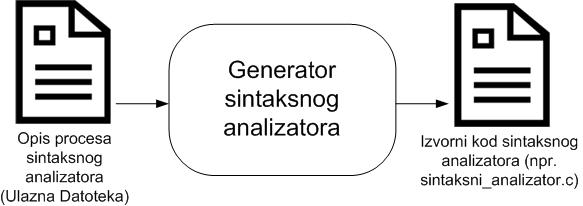
\includegraphics[width=0.7\textwidth]{slike/generator-sintaksnog-analizatora.jpg}
\caption{Način rada generatora sintaksnog analizatora.}
\label{fig:generator-sintaksnog-analizatora}
\end{figure}

Način rada generatora sintaksnog analizatora analogan je načinu rada generatora leksičkog analizatora iz prve vježbe i prikazan je na slici \ref{fig:generator-sintaksnog-analizatora}.
Generator sintaksnog analizatora kojeg je potrebno ostvariti treba prihvaćati opis procesa sintaksnog analizatora zadan tekstualnom datotekom (dalje Ulazna Datoteka).
Rezultat izvođenja generatora treba biti sintaksni analizator, slično kao u prvoj vježbi.
U praksi generatori sintaksnih analizatora kao izlaz daju izvorni kod sintaksnog analizatora, ali kao i u prvoj vježbi, dozvolit ćemo da generator analizatoru potrebne podatke predaje putem datoteke ili na neki sličan način.
Ulazna Datoteka bit će zadana u sljedećem formatu: 

\begin{description}
\itemsep 1pt
\item \%V \emph{nezavršni znakovi gramatike}
\item \%T \emph{završni znakovi gramatike}
\item \%Syn \emph{sinkronizacijski završni znakovi}
\item \emph{produkcije gramatike}
\end{description}

U nastavku je objašnjeno kako pojedini dio datoteke treba izgledati.
Zbog jednostavnosti implementacije, generator sintaksnog analizatora može pretpostaviti da je Ulazna Datoteka ispravno zadana u skladu s pravilima opisanim u ovom dokumentu.

\subsection{Nezavršni znakovi gramatike}

Prvi redak Ulazne Datoteke započinje znakovima \verb|%V| i točno jednim razmakom nakon čega slijede jedan ili više nezavršnih znakova gramatike odvojeni točno jednim razmakom.
Svaki nezavršni znak gramatike pojavit će se u ovom retku točno jednom.
Ime nezavršnog znaka sastoji se od jednog ili više malih i velikih slova engleske abecede i znakova \verb|_| (underscore) okruženih trokutastim zagradama.
Trokutaste zagrade su sastavni dio nezavršnog znaka i služe za jednostavno razlikovanje nezavršnih i završnih znakova.
Prvi navedeni nezavršni znak je \textbf{početni nezavršni znak gramatike}.

Na primjer, prvi redak Ulazne Datoteke može izgledati ovako:

\verb|%V <Program> <Naredba> <primarni_izraz>|

U prikazanom primjeru, \verb|<Program>| je početni nezavršni znak gramatike.

\subsection{Završni znakovi gramatike}

U drugom retku Ulazne Datoteke navedeni su završni znakovi gramatike.
Redak počinje znakovima \verb|%T| i točno jednim razmakom nakon čega slijede jedan ili više završnih znakova gramatike odvojeni točno jednim razmakom.
Svaki završni znak gramatike bit će naveden točno jednom.
Završni znakovi gramatike su uniformni znakovi koje generira leksički analizator te su istog oblika kao imena uniformnih znakova.
Drugim riječima, imena završnih znakova će se sastojati od malih i velikih slova engleske abecede i znakova \verb|_| (underscore).

Na primjer, drugi redak Ulazne Datoteke može izgledati ovako:

\verb|%T IDENTIFIKATOR brojcanaKonstanta znakovnaKonstanta OP_PLUS|

\subsection{Sinkronizacijski završni znakovi}

U trećem retku Ulazne Datoteke navedeni su sinkronizacijski završni znakovi.
Generirani parser treba ove znakove koristiti u postupku oporavka o pogreške.
Postupak oporavka od pogreške opisan je kasnije u poglavlju \ref{sec:syn_oporavak}.

Redak započinje znakovima \verb|%Syn| i točno jednim razmakom nakon čega slijede jedan ili više završnih znakova gramatike odvojeni točno jednim razmakom.

Na primjer, treći redak Ulazne Datoteke može izgledati ovako:

\verb|%Syn TOCKAZAREZ ZAREZ|

\subsection{Produkcije gramatike}
U nastavku Ulazne Datoteke navedene su produkcije gramatike.
Lijeve strane produkcije sastoje se od točno jednog nezavršnog znaka koji stoji sam u retku čiji početni znak je lijeva trokutasta zagrada nezavršnog znaka (vidi primjer).
Nakon retka s lijevom stranom produkcije slijedi jedan ili više redaka koji započinju točno jednim znakom razmaka i predstavljaju desnu stranu produkcije.
Desna strana svake produkcije sastoji se od jednog ili više završnih ili nezavršnih znakova odvojenih točno jednim razmakom.
Desna strana epsilon produkcije prikazuje se retkom koji počinje znakom razmaka nakon kojeg slijedi znak \verb|$| (dolar).

Na primjer, produkcije gramatike mogu izgledati ovako:
\begin{lstlisting}[caption={Primjer produkcija gramatike.},label=lst:produkcije_gramatike_primjer]
<A>
 <B> <C> c
<B>
 $
 b <C> <D> <E>
<A>
 e <D> <B>
<C>
 <D> a <B>
 c a
<D>
 $
 d <D>
<E>
 e <A> f
 c
\end{lstlisting}

Na ovaj način prikazana je gramatika (opisana BNF notacijom):
\begin{lstlisting}[caption={Primjer produkcija gramatike u BNF notaciji.},label=lst:produkcije_gramatike_primjer_bnf]
<A> ::= <B> <C> c | e <D> <B>
<B> ::= "" | b <C> <D> <E>
<C> ::= <D> a <B> | c a
<D> ::= "" | d <D>
<E> ::= e <A> f | c
\end{lstlisting}

Cjeloviti primjer Ulazne Datoteke koja opisuje gramatiku sa 100.~stranice udžbenika nalazi se \href{https://github.com/fer-ppj/ppj-labosi/raw/master/res/lab2/gramatika100.san}{ovdje}.
Nad zadanom gramatikom je u udžbeniku prikazan način računanja ZAPOČINJE skupova.
Sinkronizacijski znak je odabran nasumično kako bi se zadovoljila pravila za oblik Ulazne Datoteke.

\subsection{Zadaci generatora sintaksnog analizatora}
Generator sintaksnog analizatora treba pročitati Ulaznu Datoteku i izgraditi tablice Akcija i NovoStanje odgovarajućeg kanonskog LR(1) parsera.
Generator treba izgrađene tablice ugraditi u zasebno razvijen sintaksni analizator.
Tablice parsera mogu se ugraditi u sintaksni analizator na više načina isto kao što su se tablice konačnog automata ugrađivale u leksički analizator u prvoj laboratorijskoj vježbi.

Algoritam izgradnje tablica LR(1) parsera opisan je od stranice 148 udžbenika.
Algoritam počinje dodavanjem novog početnog nezavršnog znaka i nove produkcije u zadanu gramatiku.
Ovaj postupak opisan je u fusnoti na stranici 140 udžbenika.
U teoretskom smislu, ako se originalni početni nezavršni znak gramatike ne pojavljuje s desne strane niti jedne produkcije, nije nužno dodavati novi početni nezavršni znak.
Zbog uniformnosti, u ovoj laboratorijskoj vježbi generator LR(1) parsera \textbf{uvijek treba dodati novi početni nezavršni znak i odgovarajuću produkciju}.

Algoritam nastavlja izgradnjom nedeterminističkog konačnog automata s epsilon prijelazima.
Stanja automata označena su LR(1) stavkama.
Zbog uniformnosti oznaka stanja, nije potrebno u $\varepsilon$-NKA ugraditi stanje $q_{0}$, nego se za početno stanje može koristiti LR(1) stavka koja proizlazi iz dodane produkcije koja iz novog početnog nezavršnog znaka generira originalni početni nezavršni znak gramatike zadan u Ulaznoj Datoteci.
U ovom slučaju, automat sa i bez stanja $q_{0}$ potpuno su ekvivalentni tj.~prihvaćaju isti jezik.

Prilikom izgradnje automata, nužno je računati ZAPOČINJE skupove za nizove znakova.
Način računanja ZAPOČINJE skupova opisan je na 102.~stranici udžbenika.
Za potrebe generiranja LR(1) parsera potrebno je proširiti domenu ZAPOČINJE skupova sa desnih strana produkcije na bilo koji sufiks desne strane produkcije (ili jednostavno na proizvoljne nizove završnih i nezavršnih znakova).
Algoritam računanja ostaje potpuno isti.
Dodatno, za generiranje LR(1) parsera \textbf{nije potrebno} određivati SLIJEDI skupove.

Dobiveni $\varepsilon$-NKA treba pretvoriti u istovjetni DKA.
Postupak pretvorbe $\varepsilon$-NKA u DKA opisan je u udžbeniku “Uvod u teoriju računarstva”.
Stanja DKA označena su skupovima LR(1) stavki.
Iz stanja i prijelaza DKA popunjavaju se tablice {\em Akcija} i {\em NovoStanje}.

\subsection{Razrješavanje nejednoznačnosti}
Iako je klasa LR(1) jezika široka i odgovara klasi determinističkih kontekstno neovisnih jezika (jezici koje može prepoznati deterministički potisni automat), pojedine konstrukte iz mnogih programskih jezika teško je opisati LR(1) gramatikom bez bitnog usložnjavanja gramatike ili je uopće nemoguće napisati odgovarajuću gramatiku.
S obzirom da je složenost gramatike važna za semantičku analizu, pokazuje se da je dobro rješenje zadati gramatiku s pažljivo odabranim nejednoznačnostima koje se onda razriješe ili ručno ili koristeći jednostavna pravila koja su opisana u nastavku.

Nejednoznačnosti u gramatici u gradnji LR(1) parsera očituju se kroz {\em Pomakni/Reduciraj} i {\em Reduciraj/Reduciraj} proturječja.
{\em Pomakni/Reduciraj} proturječje izgrađeni generator treba razriješiti u korist akcije Pomakni.
{\em Reduciraj/Reduciraj} proturječje potrebno je razriješiti u korist one akcije koja reducira produkciju zadanu ranije u Ulaznoj Datoteci.
Poželjno je da generator korisniku ispiše gdje je došlo do proturječja i kako je proturječje razriješeno\footnote{Ovo se očito \emph{neće} provjeravati pri automatskoj evaluaciji rješenja na sustavu SPRUT.}.

\section{Sintaksni analizator}
Uloga sintaksnog analizatora u ovoj laboratorijskoj vježbi bit će parsiranje niza uniformnih znakova.
Drugim riječima, sintaksni analizator treba provjeravati zadovoljava li niz uniformnih znakova sintaksna pravila zadana gramatikom u Ulaznoj Datoteci i konstruirati generativno stablo za dani program.
Sintaksni analizator treba generativno stablo ispisati na standardni izlaz prema uputi u poglavlju \ref{sec:syn_ispis}.
U nastavku je opisan način rada sintaksnog analizatora kojeg je potrebno ostvariti za ovu laboratorijsku vježbu.

\subsection{Ulaz u sintaksni analizator}
Analizator čita niz uniformnih znakova sa standardnog ulaza.
Niz uniformnih znakova bit će oblikovan identično kao izlaz iz prve laboratorijske vježbe.
U ulazu će se pojavljivati isključivo oni uniformni znakovi koji su definirani kao završni znakovi gramatike u Ulaznoj Datotoeci koja je predana generatoru.
Leksičke jedinke neće započinjati ili završavati znakom praznine ili tabom i neće se protezati kroz više redaka, ali mogu sadržavati praznine (vidi primjere).

Za sam postupak sintaksne analize važni su jedino uniformni znakovi, a broj retka i leksička jedinka služe za prijavljivanje grešaka i dodatno za ispis generativnog stabla kao što je opisano u nastavku.

\subsection{Simulator LR parsera}
Središnji algoritam generiranog sintaksnog analizatora je simulator LR parsera.
Koristeći tablice {\em Akcija} i {\em NovoStanje}, simulator čita uniformne znakove iz niza uniformnih znakova i provjerava sintaksnu ispravnost ulaznog programa u jezični procesor.
Dodatno, simulator gradi generativno stablo niza uniformnih znakova.
Listovi generativnog stabla označeni su uniformnim znakovima ili epsilonom (znakom \verb|$|) u slučaju da list predstavlja desnu stranu \(\varepsilon\)-produkcije.
Kad bi se generativno stablo obišlo dubinskim pretraživanjem uz obradu djece s lijeva na desno i uz ispisivanje listova, opet bismo dobili (isti) niz uniformnih znakova (epsilon predstavlja prazan niz).
Uz sam uniformni znak, list generativnog stabla treba biti označen i retkom u kojem se pripadna leksička jedinka nalazila u ulaznom programu i samom leksičkom jedinkom\footnote{Alternativno, list može biti označen i nekim drugim podacima pomoću kojih je moguće rekonstruirati ova tri podatka.}.
Unutrašnji čvorovi generativnog stabla su označeni nezavršnim znakovima zadane gramatike.

U ovoj laboratorijskoj vježbi, generativno stablo gradit će se eksplicitno.
S tim ciljem, na stogu simulatora LR parsera trebaju se nalaziti čvorovi generativnog stabla (uz ostale podatke nužne za rad samog simulatora).
Prilikom provođenja akcije {\em Pomakni}, simulator gradi novi list generativnog stabla i označava ga u skladu s ranijim opisom.
Prilikom provođenja akcije {\em Reduciraj}, simulator gradi novi unutrašnji čvor stabla i čvorove sa stoga koji odgovaraju uzorku za zamjenu povezuje kao djecu novog unutrašnjeg čvora.
U skladu s pravilima rada simulatora LR parsera, uzorak za zamjenu uklanja se sa stoga i zamjenjuje se znakom lijeve strane produkcije uz pripadno stanje i čvor stabla.
Slijedeći ovaj postupak, prilikom izvođenja akcije {\em Prihvati}, na stogu simulatora nalazit će se korjen generativnog stabla označen početnim nezavršnim znakom gramatike.

\subsection{Ispis generativnog stabla}\label{sec:syn_ispis}
U ovoj laboratorijskoj vježbi, sintaksni analizator na standardni izlaz treba ispisati konstruirano generativno stablo.
Ispis treba obaviti dubinskim obilaskom generativnog stabla, pri čemu se prvo ispisuje oznaka čvora roditelja, a nakon toga se ispisuju podstabla čiji korijeni su djeca čvora roditelja, s lijeva na desno.
Na svakoj sljedećoj razini stabla, ispis treba prefiksirati jednim dodatnim razmakom.

Pri ispisu oznaka unutrašnjih čvorova stabla treba ispisivati nezavršni znak gramatike kojim je čvor označen.
Pri ispisu oznaka listova treba ispisati ili znak \verb|$| ako se radi o čvoru označenom epsilonom ili uniformni znak, broj retka i leksičku jedinku identično kao što je ista leksička jedinka opisana u ulazu analizatoru.
Drugim riječima, nakon odgovarajućeg broja praznina (ovisno o dubini u generativnom stablu), treba ispisati uniformni znak, jedan znak razmaka, broj retka, jedan znak razmaka i leksičku jedinku.

\subsection{Oporavak od pogreške}\label{sec:syn_oporavak}
Za potrebe ove laboratorijske vježbe, u simulator LR parsera treba ugraditi jednostavan postupak oporavka od pogreške traženjem sinkronizacijskog znaka.
Kada naiđe na pogrešku u nizu uniformnih znakova, simulator treba ispisati poruku o pogrešci u kojoj su navedeni\footnote{Ovo se neće provjeravati u automatskoj evaluaciji putem sustava SPRUT, ali se može provjeravati na usmenom odgovaranju vježbe.}:

\begin{enumerate}
\item
broj retka u kojem se pogreška dogodila
\item
očekivani uniformni znakovi (oni znakovi koji ne bi izazvali pogrešku)
\item
pročitani uniformni znak iz niza uniformnih znakova i odgovarajući znakovni prikaz iz izvornog koda programa (dohvaćen iz tablice znakova).
\end{enumerate}

Nakon ispisa pogreške, simulator treba preskočiti sve znakove u nizu uniformnih znakova do prvog sljedećeg sinkronizacijskog znaka.
Sinkronizacijski znakovi za gramatiku definirani su u Ulaznoj Datoteci.
Kada je pronašao prvi sljedeći sinkronizacijski znak, simulator sa stoga odbacuje stanja (i pripadne podatke i čvorove stabla) dok ne dođe do nekog stanja s u kojem je definirana $Akcija[s, sinkronizacijski\_znak]$.
Nakon toga simulator nastavlja s normalnim radom\footnote{Ovaj postupak oporavka od pogreške vrlo je jednostavan, ali očito daje i vrlo slabe rezultate, tj.~za veliku većinu sintaksnih pogrešaka oporavak neće biti osobito uspješan.}.

\section{Primjeri}
U ispisu \ref{lst:ulazna_datoteka_148} je prikazana Ulazna Datoteka za gramatiku sa 148.~stranice udžbenika, pri čemu je izbačen nezavrnšni znak \texttt{S} i pripadna prva produkcija, a nezavršni znak \texttt{A} je postavljen za početni nezavršni znak.
Znak \texttt{S} je u toj gramatici služio kao ``novi početni nezavršni znak'', a njega sintaksni analizator iz ove vježbe samostalno dodaje.

\begin{lstlisting}[caption={Ulazna Datoteka za gramatiku sa 148.~stranice udžbenika.},label=lst:ulazna_datoteka_148]
%V <A> <B>
%T a b
%Syn b
<A>
 <B> <A>
<B>
 a <B>
 b
<A>
 $

\end{lstlisting}

Sinkronizacijski znak je ovdje arbitrarno postavljen na \verb|b|, ali na ovom primjeru nećemo promatrati oporavak od pogreške.
Završni znakovi gramatike \verb|a| i \verb|b| predstavljaju uniformne znakove leksičkih jedinki.

Primjer ulaza u sintaksni analizator generiran za prethodnu Ulaznu Datoteku prikazan je u ispisu \ref{lst:ulaz_148}.
U primjeru su nizu uniformnih znakova arbitrarno pridruženi brojevi redaka i leksičke jedine - recimo da uniformni znak \verb|a| predstavlja leksičke jedinke koje se sastoje od uzastopnih znakova \verb|x| (opcionalno odvojenih prazninama), a uniformni znak \verb|b| predstavlja leksičke jedinke koje se sastoje od uzastopnih znakova \verb|y| (opcionalno odvojenih prazninama).

\begin{lstlisting}[caption={Ulaz u analizator za gramatiku sa 148.~stranice udžbenika.},label=lst:ulaz_148]
a 1 x x x
b 2 y y
a 3 xx xx
a 4 xx xx xx
b 4 y

\end{lstlisting}

Ispis sintaksnog analizatora za dani primjer prikazan je u ispisu \ref{lst:ispis_148}.
Ispis prikazuje stvoreno generativno stablo u skladu s opisom u poglavlju \ref{sec:syn_ispis}.

\begin{lstlisting}[caption={Ispis analizatora za gramatiku sa 148.~stranice udžbenika i ulaz is ispisa \ref{lst:ulaz_148}.},label=lst:ispis_148]
<A>
 <B>
  a 1 x x x
  <B>
   b 2 y y
 <A>
  <B>
   a 3 xx xx
   <B>
    a 4 xx xx xx
    <B>
     b 4 y
  <A>
   $

\end{lstlisting}

Primjer Ulazne Datoteke generatora za podskup jezika C nalazi se \href{https://github.com/fer-ppj/ppj-labosi/raw/master/res/lab2/simplePpjLang.san}{ovdje}\footnote{Za ovaj primjer generator generira \(\varepsilon\)-NKA s 3115 stanja i 6343 prijelaza iz čega nastaje DKA sa 691 stanja i 5404 prijelaza uz jedno \emph{Pomakni/Reduciraj} proturječje vezano uz \texttt{else} dio naredbe grananja.}.
U ispisu \ref{lst:primjer_C_err} prikazan je ``C program'' sa sintaksnom pogreškom.

\begin{lstlisting}[caption={Jednostavan C program sa sintaksnom greškom.},label=lst:primjer_C_err]
int x = 3 &;
int y = 2;

\end{lstlisting}

Za prikazani program, sintaksni analizator bi na standardni ulaz dobio ulaz prikazan u nastavku.

\begin{lstlisting}[caption={Ulaz za sintaksni analizator za program \ref{lst:primjer_C_err}.},label=lst:primjer_C_err_ulaz]
KR_INT 1 int
IDN 1 x
OP_PRIDRUZI 1 =
BROJ 1 3
OP_BIN_I 1 &
TOCKAZAREZ 1 ;
KR_INT 2 int
IDN 2 y
OP_PRIDRUZI 2 =
BROJ 2 2
TOCKAZAREZ 2 ;

\end{lstlisting}

Do sintaksne greške ovdje dolazi kada analizator čita uniformni znak \verb|TOCKAZAREZ| koji odgovara znaku \verb|;| iz prvog retka programa\footnote{Ponovno, izvorni kod je ovdje prikazan samo kako bi bilo lakse pratiti primjer --- niti jedan program u ovoj vježbi neće dobiti taj izvorni kod, već će sintaksni analizator izravno dobiti niz uniformnih znakova iz ispisa \ref{lst:primjer_C_err_ulaz}}.

Kako je \verb|TOCKAZAREZ| jedan od sinkronizacijskih znakova, u postupku oporavka od pogreske se ne odbacuje niti jedan uniformni znak iz ulaza.
U drugom koraku postupka oporavka od pogreške sa stoga se izbacuje list stabla koji predstavlja znak \verb|OP_BIN_I| tj.~znak \verb|&| iz ulaznog programa.
Nakon izbacivanja tog znaka, parser može prihvatiti znak \verb|TOCKAZAREZ| pa ga i prihvaća i nastavlja s radom, tj.~postupak oporavka od pogreške je bio uspješan.

Očekivani ispis analizatora može se vidjeti \href{https://github.com/fer-ppj/ppj-labosi/raw/master/res/lab2/simplePpjLang_err.out}{ovdje}.

Svi ovi kao i nekoliko složenijih primjera nalaze se u \href{https://github.com/fer-ppj/ppj-labosi/raw/master/res/lab2/langdefs.zip}{ovoj arhivi}.
Za jednostavnije primjere je dana i datoteka imena \verb|*_gen.txt| koja sadrži dio kontrolnog ispisa generatora što možda može biti korisno kod uklanjanja pogrešaka pri razvoju generatora.
U tim datotekama su navedene izračunate relacije i generirani konačni automati, a za najjednostavniji primjer i tablice LR-parsera.

Ulazne Datoteke za generator u arhivi imaju nastavak \verb|.san|, a ulazi i očekivani ispisi iz analizatora imaju nastavke \verb|.in| i \verb|.out|.
Dodatno, uz primjere je priložen i \verb|.gif| generativnog stabla kako biste mogli dobiti osjećaj za to kako stablo izgleda, pogotovo za primjer podskupa jezika C što će biti važno za treću laboratorijsku vježbu.

\section{Savjeti za implementaciju}
U ovom poglavlju navedene su neke napomene koje mogu pomoći u ostvarenju ove laboratorijske vježbe.
Poglavlje će biti prošireno ako se za tim pokaže potreba u skladu sa čestim pitanjima.

\subsection{Računanje refleksivnog tranzitivnog okruženja relacije}
Prilikom računanja skupova ZAPOČINJE, potrebno je izračunati relaciju {\em ZapočinjeZnakom} koja je refleksivno tranzitivno okruženje relacije {\em ZapočinjeIzravnoZnakom}.
Na stranici 102 udžbenika na visokoj razini je opisano kako se spomenuto okruženje može izračunati.
Korisno je relaciju {\em ZapočinjeZnakom} zamisliti kao usmjereni graf u kojem su znakovi čvorovi, a bridovi su članovi relacije {\em ZapočinjeZnakom}.
Drugim riječima, ako i samo ako je u tablici relacije {\em ZapočinjeZnakom} za neki par znakova navedena jedinica, ti znakovi su u grafu spojeni usmjerenim bridom.
Neki par znakova (X, Y) će biti u tranzitivnom okruženju dane relacije ako i samo ako u usmjerenom grafu postoji put od znaka X do znaka Y.
Dodatno, s obzirom da tražimo {\em refleksivno} tranzitivno okruženje, u relaciji će biti i svi parovi (X, X).

U skladu s ovom interpretacijom, postupak računanja opisan u knjizi trebalo bi ponavljati iterativno dok god se tablica nove relacije ne prestane mijenjati ili jednostavno ponoviti ga {\em n} puta gdje je {\em n} dimenzija tablice.
Također, bilo koji drugi postupak za traženje puteva u grafu može se iskoristiti za računanje nove relacije.

\section{Predaja druge laboratorijske vježbe}
Predaja druge laboratorijske vježbe na sustav SPRUT odvijat će se isto kao predaja prve laboratorijske vježbe.

Rješenje treba biti zapakirano u \texttt{zip} arhivu pri čemu se programski kod generatora nalazi u korijenskom direktoriju arhive.
Nakon prevođenja i izvođenja generatora, u poddirektoriju \texttt{analizator} treba se nalaziti sve potrebno za prevođenje i izvođenje sintaksnog analizatora.

Ulazna točka u generator za Javu treba biti u razredu \texttt{GSA}, a ulazna točka u analizator u razredu \texttt{SA}.
Za Python, ulazna točka u generator će biti datoteka \texttt{GSA.py}, a ulazna točka u analizator datoteka \texttt{SA.py}.
Za ostale jezike (uključujući C\#), imena datoteka su proizvoljna.

\emph{Napomena:} predano rješenje za drugu vježbu ni na koji način ne ovisi o prvoj vježbi. Ulaz u sintaksni analizator u ovoj vježbi je niz uniformnih znakova u skladu s prethodnim opisom i nigdje u ovoj vježbi ne baratamo s izvornim kodom programa. Zato nemojte spajati leksički analizator s rješenjem ove vježbe i očekivati izvorni kod na ulazu.


\chapter{Treća laboratorijska vježba}\label{chap:III}
Tema treće laboratorijske vježbe je semantička analiza.
Za razliku od prve dvije vježbe gdje je cilj bio ostvariti generator leksičkog odnosno sintaksnog analizatora, u ovoj vježbi je cilj ostvariti semantički analizator za jedan zadani programski jezik.
Važno je uočiti da je ova vježba potpuno neovisna o rješenjima prve dvije vježbe.

Kako je semantička analiza tipično složenija od leksičke i sintaksne analize, među ostalim i zbog teže primjenjive formalne podloge, programski jezik koji će se koristiti u ovoj vježbi je semantički relativno jednostavan.
Dodatno, neka ograničenja koja bi tipično bila u domeni semantičke analize prebačena su u sintaksnu analizu, opet s ciljem pojednostavljivanja semantičke analize.
Nadalje, iako se semantička analiza tipično provodi nad sintaksnim stablom\footnote{Tipično sintaksni analizator izravno generira sintaksno stablo ili se sintaksno stablo izgradi naknadnim obilaskom generativnog stabla.}, za potrebe laboratorijskih vježbi ćemo ovaj korak preskočiti, tj.~semantička analiza će se provoditi nad generativnim stablom.
U ovoj uputi navode se samo semantička pravila koja su važna za semantičku analizu, a pravila će biti dodatno proširena u uputi za sljedeću laboratorijsku vježbu za potrebe generiranja koda.

Uz sva pojednostavljenja, opis semantike svakog programskog jezika (pa tako i ovog) je inherentno relativno složen.
Na primjer, u \emph{C} standardu opis jezika (bez standardnih biblioteka) ima nešto manje od 200 stranica, a od toga se većina bavi semantikom.
Naravno, \emph{C} je daleko složeniji jezik od jezika kojim se bave ove laboratorijske vježbe i opis ovog jezika nije ni približno toliko potpun, ali je istovremeno znatno jednostavniji za potrebe implementacije semantičkog analizatora.
Cilj upute je da većina pravila bude očita nakon prvog čitanja, a da istovremeno što veći dio jezika bude pokriven, tj.~da ne bude nužno postavljati mnogo pitanja tipa ``A što ako\ldots?''.

\section{Ulaz i ispis semantičkog analizatora}
Semantički analizator će na stadardni ulaz dobiti generativno stablo u istom obliku kao ispis sintaksnog analizatora iz druge laboratorijske vježbe.
Usprkos tome, u većini primjera kojima se u uputi ilustrira neko semantičko pravilo prikazuje se program a ne generativno stablo.
Program \textbf{nije} ulaz u rješenje ove laboratorijske vježbe, ali je semantička pravila lakše objasniti nad programom nego nad relativno nepreglednim generativnim stablom.
Iz tog razloga se za testiranje rješenja tijekom razvoja preporuča korištenje leksičkog i sintaksnog analizatora kako biste mogli rad semantičkog analizatora provjeravati nad programima i kako ne biste morali ručno mijenjati generativno stablo.

Za ovaj način rada ne morate mijenjati rješenja prošlih laboratorijskih vježbi ni na koji način.
Ulazna datoteka koja opisuje leksički analizator jezika \emph{ppjC} nalazi se \href{https://github.com/fer-ppj/ppj-labosi/raw/master/res/lab3/ppjC.lan}{ovdje}\footnote{Ovo je ista datoteka kao \texttt{simplePpjLang.lan}}, a ulazna datoteka koja opisuje sintaksni analizator jezika \emph{ppjC} nalazi se \href{https://github.com/fer-ppj/ppj-labosi/raw/master/res/lab3/ppjC.san}{ovdje}\footnote{Ovo je malo pojednostavljena inačica datoteke \texttt{simplePpjLang.san}. Generator generira \(\varepsilon\)-NKA s 2936 stanja i DKA s 543 stanja.}.
Koristeći ove dvije datoteke i rješenja prethodnih laboratorijskih vježbi možete generirati leksički i sintaksni analizator za jezik \emph{ppjC}.
Nadalje, kako analizatori čitaju ulaz sa stadnardnog ulaza i ispisuju rezultat izvođenja na standardni izlaz, a ulazi i izlazi su im kompatibilni, analizatore možete povezati u ``lanac'' u naredbenom retku.

Ako pretpostavimo da je \emph{LA} ime izvodivog leksičkog analizatora, \emph{SA} ime izvodivog sintaksnog analizatora i \emph{SemantickiAnalizator} ime izvodivog semantičkog analizatora (na kojem radite u ovoj vježbi), onda bi naredba kojom možete testirati rad semantičkog analizatora nad programom izgledala na primjer ovako:\\
\emph{LA} \verb#<program.c |# \emph{SA} \verb#|# \emph{SemantickiAnalizator}

Semantički analizator treba obići generativno stablo i na standardni izlaz ``ispisati produkciju'' u kojoj je otkrivena prva semantička pogreška, kao što je precizno definirano u poglavlju \ref{sec:obilazak}.
Semantički analizator ne treba provoditi nikakav postupak oporavka od pogreške.
Drugim riječima, čim otkrije prvu semantičku pogrešku i obavi odgovarajući ispis, semantički analizator prestaje s radom.

Ako je program prikazan generativnim stablom na ulazu semantički ispravan, semantički analizator ne smije ispisati ništa na standardni izlaz\footnote{Isto kao u prethodnim vježbama, sav ostali ispis, na primjer smislenije poruke o pogrešci namijenjene korisnicima cjelovitog kompilatora, mora ići na standardni izlaz za greške, tj.~\texttt{stderr}.}.


\section{Predaja treće laboratorijske vježbe}
Za predaju treće laboratorijske vježbe, sve datoteke s programskim kodom treba zapakirati u \verb|zip|-arhivu.
Ostala pravila jednaka su kao za prethodne vježbe, osim što više nije potreban direktorij \verb|analizator|.

Ulazna točka za Javu treba biti u razredu \verb|SemantickiAnalizator|, a ulazna točka za Python treba biti u datoteci \verb|SemantickiAnalizator.py|.
Za ostale jezike imena datoteka i razreda su proizvoljna.


\section{Opis jezika \emph{ppjC}}
U ovom poglavlju dan je pregled jezika kako bi se olakšalo praćenje semantičkih pravila u poglavlju \ref{sec:semanticka_pravila}.
Neki dijelovi ovog opisa možda neće biti odmah jasni, ali bit će dodatno razjašnjeni kroz opis semantičkih pravila.

\subsection{Tipovi podataka}
Jezik \emph{ppjC} ima vrlo jednostavan sustav tipova što značajno olakšava semantičku analizu.
U nastavku poglavlja navedeni su tipovi podataka u jeziku i objašnjeno je na koje načine se vrijednosti jednog tipa mogu implicitno ili eksplicitno (\emph{cast} operatorom) pretvoriti u vrijednosti drugog tipa.

\subsubsection{Brojevni tipovi}
Jezik \emph{ppjC} ima dva brojevna tipa: \verb|char| i \verb|int|.
Raspon vrijednosti tipa \verb|char| je 0--255 (8b NBC).
Tip \verb|int| koristi 32 bita i predstavlja i nenegativne cijele brojeve (pozitivne cijele brojeve i nulu) i negativne cijele brojeve u dvojnom komplementu.
Drugim riječima, raspon vrijednosti tipa \verb|int| je \(-2^{31} = -2147483648 \le v \le 2147483647 = 2^{31} - 1\).

U ostatku upute će se brojevni tipovi označavati sa \emph{T}, tj.~\emph{T} može biti \verb|char| ili \verb|int|.

\subsubsection{const-kvalifikator}
Brojevni tip prefiksiran ključnom riječi \verb|const| (uniformni znak \verb|KR_CONST|) naziva se \verb|const|-kvalificiran tip i u ostatku upute će biti označavan sa \emph{const}(\emph{T}) gdje je \emph{T} ili \verb|char| ili \verb|int|.
Varijablu \verb|const|-kvalificiranog tipa obavezno se mora inicijalizirati pri definiciji i tada pridružena vrijednost ne može se promijeniti tijekom izvođenja programa.

U ostatku upute će se brojevni tip s opcionalnim \verb|const|-kvalifikatorom označavati znakom \emph{X}, tj.~\emph{X} može biti \verb|char|, \verb|int|, \emph{const}(\verb|char|) ili \emph{const}(\verb|int|).
Koristeći oznaku \emph{T}, \emph{X} može biti \emph{T} ili \emph{const}(\emph{T}).

\subsubsection{Nizovi (engl.~\emph{array})}
Jezik podržava nizove isključivo brojevnih tipova (\verb|const|-kvalificiranih ili ne).
Drugim riječima, ne postoje nizovi nizova (tj.~višedimenzionalni nizovi), a ovo ograničenje je osigurano u gramatici, tj.~sintaksnoj analizi.
Tip \emph{niz} se u uputi označava sa \emph{niz}(\emph{X}) gdje je \emph{X} neki (možda \verb|const|-kvalificiran) brojevni tip.

\subsubsection{void}
Ključna riječ \verb|void| ima vrlo sličnu ulogu kao u jeziku \emph{C}, a kao tip može biti isključivo povratni tip funkcije.

\subsubsection{Tip funkcija}
Tip funkcije određen je tipom povratne vrijednosti i svih formalnih parametara.
Na primjer, funkcije u ispisu \ref{lst:primjer_tip_funkcije} redom imaju tipove \emph{funkcija}(\verb|[char|, \verb|char]| \(\to\) \verb|int|), \emph{funkcija}(\verb|[int]| \(\to\) \verb|void|) i \emph{funkcija}(\verb|void| \(\to\) \verb|void|).
Tipovi parametara organizirani su u listu, a ako funkcija nema parametara, to je označeno sa \verb|void| (ali ne sa \verb|[void]|, što ne bi imalo smisla).

\begin{lstlisting}[caption={Primjer jednostavne funkcije.},label=lst:primjer_tip_funkcije]
int f1(char a, char b) {
    return a == b;
}

void f2(int x) {
    return;
}

void f3(void) {
    return;
}
\end{lstlisting}

\subsubsection{Implicitne promjene tipa}
Sve vrijednosti tipa \emph{const}(\emph{T}) mogu se implicitno pretvoriti u vrijednost tipa \emph{T}\footnote{Važno je uočiti da se promjene tipa (i implicitne i eksplicitne) odvijaju nad \textbf{vrijednostima} a ne nad \textbf{varijablama}. Tip varijable koji je određen njenom definicijom nije moguće nikako promijeniti.}.
Vrijedi i obrat, tj.~sve vrijednosti tipa \verb|int| ili \verb|char| mogu se implicitno pretvoriti u vrijednosti odgovarajućeg \verb|const|-kvalificiranog tipa.

Nadalje, sve vrijednosti tipa \verb|char| mogu se implicitno pretvoriti u vrijednost tipa \verb|int|.
Kako \verb|int| sadrži raspon tipa \verb|char| kao podskup svog raspona, pri ovoj implicitnoj promjeni sama vrijednost se ne mijenja.

Konačno, vrijednost tipa \emph{niz}(\emph{T}) gdje \emph{T} \textbf{nije} \verb|const|-kvalificiran tip može se pretvoriti u vrijednost tipa \emph{niz}(\emph{const}(\emph{T})).

U semantičkim pravilima u nastavku upute, izraz \emph{U} \(\sim\) \emph{V} je zadovoljen ako se vrijednost tipa \emph{U} može implicitno pretvoriti u vrijednost tipa \emph{V}, a inače se radi o semantičkoj pogrešci.
Relacija \(\sim\) je refleksivna i tranzitivna.

\subsubsection{Logički podtip tipa \texttt{int}}
Logički tip u jeziku \emph{ppjC} nije poseban tip nego je podtip tipa \verb|int| s vrijednostima \verb|0| i \verb|1|, pri čemu \verb|0| predstavlja logičku neistinu, a \verb|1| logičku istinu.
Sve vrijednosti različite od nule pretvaraju se u logičku vrijednost \verb|1|, a nula se ``pretvara'' u logičku vrijednost \verb|0|\footnote{Ova rečenica ni na koji način ne utječe na semantičku analizu u ovoj laboratorijskoj vježbi, ali će biti važna za generiranje koda u sljedećoj vježbi.}.

\subsubsection{Eksplicitne promjene tipa}\label{sec:semantika_cast}
Eksplicitne promjene tipa dozvoljene su samo nad vrijednostima brojevnih tipova, a zadaju se \emph{cast} operatorom.
Drugim riječima, jedina promjena tipa koju je moguće ostvariti samo eksplicitno je promjena iz vrijednosti tipa \verb|int| u vrijednost tipa \verb|char|.
Ako iznos \verb|int| vrijednosti nije u opsegu tipa \verb|char|, \textbf{rezultat operacije nije definiran}\footnote{Vidi \ref{sec:UB}.}, a u suprotnom se iznos ne mijenja.

\subsection{Konstante}\label{sec:semantika_konstante}
Brojevne konstante (uniformni znak \verb|BROJ|) su tipa \verb|int| i moraju imati vrijednost u dozvoljenom rasponu za tip \verb|int|.

Znakovne konstante (uniformni znak \verb|ZNAK|) su tipa \verb|char| i imaju vrijednost jednaku ASCII kodu znaka.
Kroz leksičku analizu proći će i neke znakovne konstante koje nisu ispravne pa takve pogreške treba otkriti u semantičkoj analizi.
Konkretno, od znakovnih konstanti koje između jednostrukih navodnika imaju više od jednog znaka (tj.~imaju znak prefiksiran znakom \verb|\|), \emph{ppjC} dozvoljava isključivo znakove \verb|'\t'|, \verb|'\n'|, \verb|'\0'|, \verb|'\''| (jednostruki navodnik), \verb|'\"'| (dvostruki navodnik) i \verb|'\\'|.
Sve ostale dvoznačne konstante predstavljaju semantičku grešku\footnote{Ovo pravilo se dakako moglo osigurati i u leksičkoj analizi, ali je namjerno ostavljeno za semantičku analizu kako bi se ilustriralo da leksička, sintaksna i semantička pravila nisu zadana nekim univerzalnim kanonom, nego autor jezičnog procesora mora odlučiti koje značajke će provjeravati na koji način. Ovo svakako nije previše uobičajen primjer jer je vrlo lako uključiti ovo pravilo u regularne izraze, ali na primjer provjera raspona brojevnih konstanti je značajno jednostavnija u domeni semantičke analize nego u ovakvom modelu leksičke analize.}.
Nadalje, znak dvostrukog navodnika se može pojaviti neprefiksiran (dakle \verb|'"'|) sa istim značenjem.

Konstantni znakovni nizovi (uniformni znak \verb|NIZ_ZNAKOVA|) su tipa \emph{niz}(\emph{const}(\verb|char|)) i implicitno završavaju znakom \verb|'\0'| (kao u \emph{C}-u).
Ispravni konstantni znakovini nizovi počinju i završavaju dvostrukim navodnikom (ovo je osigurano leksičkom analizom), i mogu sadržavati sve ispisive ASCII znakove, a znakom \verb|\| mogu biti prefiksirani samo znakovi koji su navedeni u prethodnom odlomku.
Slično kao za znakovne konstante, leksička analiza će propustiti neke konstantne znakovne nizove koji nisu ispravni, npr.~nizove \verb|"\"| i \verb|"\x"|.

\subsection{Djelokrug deklaracija i životni vijek varijabli}
Jezik \emph{ppjC} po klasifikaciji iz udžbenika koristi \emph{statičko pravilo djelokruga bez ugniježđenih procedura} \cite[str.~223--224]{udzbenik}, ali podržava ugniježđene blokove, isto kao \emph{C}.
Kako je sintaksa procedura u udžbeniku bliska \emph{Pascalu}, a taj stil danas više nije previše zastupljen i mnogi od vas se možda s njim nisu prije susreli, za potrebe laboratorijskih vježbi se oslonite više na djelokrug deklaracija \emph{C}-a i na primjere u nastavku.

Životni vijek globalnih varijabli počinje u trenutku njihove definicije, a završava na kraju izvođenja programa.
Za varijable lokalne nekom bloku (što uključuje i parametre funkcija), životni vijek počinje njihovom definicijom i završava na kraju tog bloka.
Varijable koje nisu eksplicitno inicijalizirane (prilikom definicije ili kasnije) imaju \emph{neodređenu vrijednost} (drugim riječima, mogu imati bilo koju vrijednost) i rezultat korištenja takve vrijednosti u bilo kakvom izrazu nije definiran\footnote{Za razliku od jezika \emph{C}, ovo se odnosi i na varijable u globalnom djelokrugu.}.

\begin{lstlisting}[caption={Jednostavan primjer djelokruga deklaracija.},label=lst:primjer_djelokrug_1]
int x = 3;
int main(void) {
    int y = x + 1; // 4
    return 0;
}
\end{lstlisting}

Jednostavan primjer prikazan je u ispisu \ref{lst:primjer_djelokrug_1}.
Varijabla \verb|x| deklarirana je u globalnom djelokrugu u kojem je deklarirana i funkcija \verb|main|.
Tijelo funkcije \verb|main| je blok, tj.~složena naredba, te kao takvo ima vlastiti djelokrug deklaracija u kojem je deklarirana varijabla \verb|y|.
U tijelu funkcije \verb|main|, prethodno deklarirana imena iz globalnog djelokruga (u ovom slučaju \verb|x|) također su dostupna.

\begin{lstlisting}[caption={Primjer pogreške u djelokrugu---varijabla \texttt{x} nije deklarirana prije korištenja.},label=lst:primjer_djelokrug_2]
int main(void) {
    int y = x + 1; // greska
    return 0;
}
int x = 3;
\end{lstlisting}

Primjer u ispisu \ref{lst:primjer_djelokrug_2} sadrži semantičku pogrešku u retku \verb|2| jer varijabla \verb|x| nije prethodno deklarirana.

\begin{lstlisting}[caption={Sakrivanje globalne deklaracije.},label=lst:primjer_djelokrug_3]
int x = 3;
int main(void) {
    int x = 5;
    int y = x + 1; // 6
    return 0;
}
\end{lstlisting}

Lokalno ime može sakriti ime iz ugniježđujućeg djelokruga.
Primjer tog slučaja prikazan je u ispisu \ref{lst:primjer_djelokrug_3}.
Deklaracija varijable \verb|x| u retku \verb|3| skriva globalnu varijablu \verb|x|.

\begin{lstlisting}[caption={Sakrivanje deklaracije u bloku.},label=lst:primjer_djelokrug_4]
int main(void) {
    int x = 3;
    int z;
    {
      int x = 5;
      int y = x + 1; // 6
      z = y + 1; // 7
    }
    z = x + 1; // 4
    return 0;
}
\end{lstlisting}

Isto pravilo zajedno s pravilom o životnom vijeku varijabli određuje značenje programa u ispisu \ref{lst:primjer_djelokrug_4}.
Važno je uočiti da je moguće sakriti samo deklaraciju iz ugniježđujućeg djelokruga, ali ne i iz istog djelokruga (u tom slučaju radi se o pokušaju redeklaracije što za varijable nije dozvoljeno, a pravila za funkcije su objašnjena u poglavlju \ref{sec:semantika_funkcije}).

Primjer ove greške prikazan je u ispisu \ref{lst:primjer_djelokrug_5}.

\begin{lstlisting}[caption={Nedozvoljena redeklaracija varijable.},label=lst:primjer_djelokrug_5]
int main(void) {
    int x = 5;
    int x = 6; // greska
    return 0;
}
\end{lstlisting}

\subsection{Funkcije}\label{sec:semantika_funkcije}
Svaki program u jeziku \emph{ppjC} mora imati funkciju s prototipom \verb|int main(void)|.
Ova funkcija je ulazna točka za izvođenje programa.

Sve funkcije koje ne primaju argumente, u deklaraciji između oblih zagrada moraju imati navedenu ključnu riječ \verb|void|.
Drugim riječima, deklaracija funkcije oblika \verb|int f();| je neispravna, a to je osigurano u gramatici tj.~u sintaksnoj analizi.

Svaka funkcija prije korištenja mora biti \textbf{deklarirana}, pri čemu je \textbf{definicija} funkcije ujedno i njena deklaracija.
Deklaracija je u tom slučaju u potpunosti završena prije znaka lijeve vitičaste zagrade koji započinje tijelo funkcije.
Funkcija može biti deklarirana proizvoljan broj puta, a mora biti definirana točno jednom.
Pritom, sve deklaracije (uključujući i definiciju) moraju imati identične povratne tipove i tipove formalnih parametara.

U deklaracijama je (za razliku od \emph{C}-a) obvezno navesti imena formalnih parametara, ali ta imena nisu važna tj.~mogu se razlikovati među različitim deklaracijama iste funkcije (drugim riječima, treba ih ignorirati).

\begin{lstlisting}[caption={Funkcija \texttt{f} nije deklarirana prije korištenja.},label=lst:primjer_deklaracija_funkcija_1]
int main(void) {
  return f(); // greska
}
int f(void) {
  return 0;
}
\end{lstlisting}

U ispisu \ref{lst:primjer_deklaracija_funkcija_1}, semantička pogreška pojavljuje se pri pozivu funkcije \verb|f| u retku \verb|2|, jer funkcija \verb|f| nije prethodno deklarirana.
Grešku je moguće ispraviti na više načina, a tri načina prikazana su u nastavku.

\begin{lstlisting}[caption={Dodatak deklaracije funkcije \texttt{f} prije definicije funkcije \texttt{main}.},label=lst:primjer_deklaracija_funkcija_2]
int f(void);
int main(void) {
  return f();
}
int f(void) {
  return 0;
}
\end{lstlisting}

Prvo, kao što je prikazano u ispisu \ref{lst:primjer_deklaracija_funkcija_2}, moguće je prije definicije funkcije \verb|main| (koja poziva funkciju \verb|f|) dodati deklaraciju funkcije \verb|f|.

Drugo, za razliku od definicija funkcija koje su dozvoljene isključivo u globalnom djelokrugu, funkcija se može deklarirati i unutar (bilo kojeg) bloka.
U ispisu \ref{lst:primjer_deklaracija_funkcija_3} deklaracija funkcije \verb|f| prebačena je iz globalnog djelokruga u tijelo funkcije \verb|main|.

\begin{lstlisting}[caption={Deklaracija funkcije \texttt{f} neposredno prije poziva u tijelu funkcije \texttt{main}.},label=lst:primjer_deklaracija_funkcija_3]
int main(void) {
  int f(void);
  return f();
}
int f(void) {
  return 0;
}
\end{lstlisting}

Kako je definicija funkcije ujedno i deklaracija, u ovom slučaju je moguće definiciju funkcije \verb|f| prebaciti prije definicije funkcije \verb|main|, kao što je prikazano u ispisu \ref{lst:primjer_deklaracija_funkcija_4}.

\begin{lstlisting}[caption={Definicija funkcije \texttt{f} je ujedno i njena deklaracija.},label=lst:primjer_deklaracija_funkcija_4]
int f(void) {
  return 0;
}
int main(void) {
  return f();
}
\end{lstlisting}

Nadalje, s obzirom na to da deklaracija funkcije završava prije lijeve vitičaste zagrade koja započinje tijelo funkcije, za ostvarenje rekurzije nije potrebno koristiti eksplicitnu deklaraciju funkcije.
Primjer semantički ispravne rekurzivne funkcije prikazan je u ispisu \ref{lst:primjer_deklaracija_funkcija_5}.

\begin{lstlisting}[caption={Rekurzivne funkcije ne treba eksplicitno deklarirati prije definicije.},label=lst:primjer_deklaracija_funkcija_5]
int fact(int n) {
  if (n > 0) {
    return n * fact(n-1);
  } else {
    return 1;
  }
}
\end{lstlisting}

Ipak, u slučaju da se dvije funkcije međusobno pozivaju, nije moguće izbjeći eksplicitnu deklaraciju jedne od njih.
Primjer takvog slučaja prikazan je u ispisu \ref{lst:primjer_deklaracija_funkcija_6}.

\begin{lstlisting}[caption={Nužna deklaracija funkcije \texttt{bar} prije definicije funkcije \texttt{foo}.},label=lst:primjer_deklaracija_funkcija_6]
int bar(int x);
int foo(int a, int b) {
  if (a > 0) {
    return a + bar(b);
  } else {
    return 0;
  }
}
int bar(int a) {
  return foo(a, a-1);
}
\end{lstlisting}

U deklaraciji funkcije \verb|bar| u retku \verb|1|, navedeno je drugačije ime formalnog parametra nego u definiciji funkcije u retku \verb|9|, ali to ne predstavlja grešku jer se imena parametara u deklaraciji ignoriraju.

Povratni tip funkcije može biti \verb|char| ili \verb|int| \textbf{bez} \verb|const|-kvalifikatora, ili \verb|void| što znači da funkcija ne vraća ništa.
Semantička je pogreška ako funkcija deklarirana da vraća \verb|void| pokuša vratiti neku vrijednost.
Nadalje, ako funkcija deklarirana da vraća neku vrijednost brojevnog tipa u nekom slijedu izvođenja ne vrati vrijednost, rezultat izvođenja nije definiran (ali se ne radi o semantičkoj pogrešci, tj.~semantički analizator ne treba provjeravati vraća li funkcija stvarno neku vrijednost u svim sljedovima izvođenja).
Ako funkcija vraća neku vrijednost, tip vrijednosti mora se moći implicitno pretvoriti u deklarirani povratni tip funkcije (ovo pravilo pokriva i \verb|void| povratni tip s obzirom na to da se niti jedan tip vrijednosti ne može implicitno pretvoriti u \verb|void|).

U ispisu \ref{lst:primjer_povratni_tipovi_1} je prikazana semantički ispravna funkcija \verb|foo| i semantički neispravna funkcija \verb|bar|.
Funkcija \verb|foo| je ispravna jer vrijedi \verb|char| \(\sim\) \verb|int|, a funkcija \verb|bar| je neispravna jer obrat ne vrijedi pa nije moguće vratiti \verb|int| vrijednost iz funkcije kojoj je povratni tip \verb|char|.

\begin{lstlisting}[caption={Ispravna funkcija \texttt{foo} i neispravna funkcija \texttt{bar}.},label=lst:primjer_povratni_tipovi_1]
int foo(void) {
  return 'a';
}

char bar(void) {
  return 97; // greska
}
\end{lstlisting}

Funkciju \verb|bar| moglo bi se ispraviti korištenjem \emph{cast} operatora, kao što je prikazano u ispisu \ref{lst:primjer_povratni_tipovi_2}.

\begin{lstlisting}[caption={Ispravljena funkcija \texttt{bar}.},label=lst:primjer_povratni_tipovi_2]
char bar(void) {
  return (char)97;
}
\end{lstlisting}

Nadalje, hoće li se \verb|return| naredba ikada izvesti ili ne nema utjecaja na semantičku ispravnost programa.
Na primjer, funkcija u ispisu \ref{lst:primjer_povratni_tipovi_3} također je neispravna, iako bi tijekom izvođenja uvijek vraćala vrijednost ispravnog tipa.

\begin{lstlisting}[caption={Ispravnost tipova povratnih vrijednosti ne ovisi o tome hoće li se određena \texttt{return} naredba ikada izvršiti ili ne.},label=lst:primjer_povratni_tipovi_3]
char bar(void) {
  if (0) {
    return 97; // greska
  } else {
    return (char)97;
  }
}
\end{lstlisting}

Prilikom poziva funkcije, \emph{vrijednost} argumenata brojevnog tipa prenosi se u odgovarajuće parametre\footnote{Način prenošenja argumenata ne utječe na ovu laboratorijsku vježbu, ali je ovdje naveden zbog cjelovitosti pregleda funkcija u jeziku \emph{ppjC}.}.
S druge strane, u formalne parametre tipa \emph{niz}(\emph{X}) koji se deklariraju sintaksom \emph{X} \verb|a[]| prenosi se \emph{adresa} argumenta.
U oba slučaja, tip vrijednosti argumenta mora se moći implicitno pretvoriti u tip odgovarajućeg parametra.

Razlika u načinu prenošenja argumenata u funkciju izeđu brojevnih tipova i nizova prikazana je u ispisu \ref{lst:primjer_parametri_val_ref}.

\begin{lstlisting}[caption={Brojevni tipovi se prenose \emph{razmjenom vrijednosti}. Nizovi se prenose \emph{razmjenom adresa}.},label=lst:primjer_parametri_val_ref]
void f(int x, int a[]) {
  x = x + 1;
  a[0] = a[0] + 1;
}

int main(void) {
  int x = 3;
  int a[8] = {0};
  f(x, a); // x == 3, a[0] == 1
  return 0;
}
\end{lstlisting}

\subsection{Operatori}
Većina operatora u jeziku \emph{ppjC} definirana je isključivo nad tipom \verb|int|, a i rezultat je tipa \verb|int|.
Jedna donekle iznenađujuća posljedica ovog pravila u kombinaciji s pravilima o pretvorbi tipova je da je program u ispisu \ref{lst:primjer_operatori_int} neispravan.
Naime, kako operator zbrajanja očekuje operande tipa \verb|int| i daje rezultat tipa \verb|int|, vrijednost varijable \verb|c| se implicitno pretvara u tip \verb|int| i zbraja se s konstantom \verb|1| (koja je tipa \verb|int|).
Rezultat operacije je opet tipa \verb|int|, a kako ne vrijedi \verb|int| \(\sim\) \verb|char|, radi se o semantičkoj pogrešci u pridruživanju.

\begin{lstlisting}[caption={Neispravan program s operatorom zbrajanja.},label=lst:primjer_operatori_int]
int main(void) {
  char c = 'a';
  c = c + 1; // greska
  return 0;
}
\end{lstlisting}

Pogreška se može lako ispraviti korištenjem eksplicitne promjene tipa, kao što je prikazano u ispisu \ref{lst:primjer_operatori_int_ispravljen}.

\begin{lstlisting}[caption={Ispravljen program iz ispisa \ref{lst:primjer_operatori_int}.},label=lst:primjer_operatori_int_ispravljen]
int main(void) {
  char c = 'a';
  c = (char)(c + 1);
  return 0;
}
\end{lstlisting}

Ako pri aritmetičkim operacijama dođe do preljeva ili podljeva, rezultat operacije nije definiran.

\section{Semantička pravila jezika \emph{ppjC}}\label{sec:semanticka_pravila}
Semantička pravila jezika definirana su u nastavku prirodnim jezikom i uz pomoć formalne notacije slične notaciji atributne prijevodne gramatike, a istovremeno je objašnjena i gramatika koja opisuje sintaksu jezika \emph{ppjC}.
Sve produkcije gramatike u BNF obliku nalaze se \href{https://github.com/fer-ppj/ppj-labosi/raw/master/res/lab3/bnf.txt}{ovdje}.
Važno je razumjeti gramatiku ovog jezika jer se semantička analiza provodi nad generativnim stablom čiji oblik izravno ovisi o gramatici.
Preporučljivo je prije čitanja semantičkih pravila pogledati produkcije gramatike i razmisliti o ulogama pojedinih znakova i produkcija.
Gramatika se sastoji od tri skupine produkcija: produkcije za izraze, produkcije za naredbenu struktura podataka i produkcije za deklaraciju i definiciju varijabli i funkcija.
Opisa semantičkih pravila u nastavku prati ovu strukturu.

\subsection{Razlika između semantičke pogreške i \emph{nedefiniranog ponašanja}}\label{sec:UB}
U nastavku ove upute, važno je razlikovati slučaj u kojem neki jezični konstrukt nije semantički ispravan i slučaj u kojem nije definiran \emph{rezultat izvođenja} tog jezičnog konstrukta. 

Kao primjer iz jezika \emph{C}, semantička je pogreška pokušati zbrojiti dva pokazivača.
Svaki ispravni \emph{C} kompilator mora odbiti prevođenje programa koji sadrži ovu semantičku pogrešku.
S druge strane, oduzimanje dva pokazivača na kompatibilne tipove semantički je ispravno i svaki ispravni \emph{C} kompilator program koji sadrži takvo oduzimanje mora prevesti (naravno, ako program ne sadrži druge pogreške).
Međutim, pojednostavljeno rečeno, ako pokazivači ne pokazuju u isti niz, \emph{rezultat oduzimanja} nije definiran (točnije, ponašanje takvog programa u cijelosti postaje nedefinirano)\footnote{Tehnički pojam za ovakav slučaj je \emph{nedefinirano ponašanje} (engl. \emph{undefined behavior}).}.

Drugi sličan primjer je dereferenciranje \emph{null} pokazivača.
U mnogim slučajevima kompilator ne može provjeriti hoće li neki pokazivač imati vrijednost \emph{null} pokazivača tijekom izvođenja programa i samim time tijekom prevođenja ne može upozoriti programera da će se to dogoditi.
Međutim, ako tijekom rada programa dođe do referenciranja \emph{null} pokazivača, ponašanje programa postaje nedefinirano sa stanovišta \emph{C} standarda.

To što je ponašanje programa u nekom slučaju nedefinirano u kontekstu izrade kompilatora znači da se o tim slučajevima ne treba posebno razmišljati (barem u okviru ove vježbe) --- tijekom izvođenja prevedenog programa, može se dogoditi bilo što, uključujući i prestanak rada kompilatora, tj.~u kontekstu ove vježbe, semantičkog analizatora.
Posljedica ove činjenice je da vaša rješenja nećemo testirati sa generativnim stablima programa koji sadrže jezične konstrukte nedefiniranog ponašanja.

\subsection{Obilazak stabla i opis semantičkih pravila}\label{sec:obilazak}
Kako generativno stablo prikazuje na koji način je iz gramatike generiran neki niz završnih znakova, struktura stabla u svakom čvoru jedinstveno određuje koja produkcija je primijenjena kako bi se znak u korijenu svakog podstabla zamijenio znakovima kojima su u stablu označena djeca tog korijena.
U ovoj laboratorijskoj vježbi se pretpostavlja provjera semantičkih pravila dubinskim pretraživanjem generativnog stabla s lijeva na desno, pri čemu se teži provjeri semantičkog pravila što je prije moguće.
To znači da se u produkcijama koje sadrže više završnih i nezavršnih znakova s desne strane produkcije, podstabla koja odgovaraju tim znakovima provjeravaju s lijeva na desno.
Nakon svake provjere nekog podstabla s desne strane produkcije, provjeravaju se sva pravila u samoj produkciji za koja su dostupna sva potrebna svojstva znakova desne strane.
Kako je redoslijed provjera važan jer o njemu ovisi ispis analizatora, uz svaku produkciju gramatike naveden je redoslijed provjere pravila.
Drugim riječima, opis obilaska u ovom odlomku je čisto informativan, tj.~služi kako bi bilo jasno zašto je u određenoj produkciji odabran baš taj redoslijed provjera pravila.

Za opis semantičkih pravila koriste se većinom izvedena i nekoliko nasljednih svojstava.
Njihova uloga je opis pravila i nije obavezno u implementaciji koristiti ista svojstva ili svojstva uopće koristiti.
Nadalje, semantička pravila nisu u potpunosti opisana pravilima računanja svojstava nego su dobrim dijelom opisana i prirodnim jezikom.
Rješenje se testira isključivo na principu ulaz\slash{}izlaz, a način ostvarenja je proizvoljan dok god će rezultat biti jednak ovom konceptualnom modelu koji je opisan u uputi.
Dakako, jedna mogućnost je implementirati upravo ovaj model obilaska stabla.

Semantička pravila navedena su po produkcijama, a produkcije su grupirane po nezavršnom znaku s lijeve strane.
Produkcije za određene grupe operatora koje imaju identičnu strukturu i semantička pravila, ali različite operatore (na primjer produkcije koje generiraju operatore zbrajanja i oduzimanja), opisane su u okviru jedne produkcije koja na mjestu operatora ima regularan izraz koji pokriva sve moguće vrijednosti (na primjer \verb#(PLUS | MINUS)#).

Nezavršni znakovi su naslovi odjeljaka, nakon čega slijedi kratak opis uloge nezavršnog znaka u gramatici i popis produkcija s pripadnim semantičkim pravilima.
Neposredno ispod svake produkcije navedena su pravila računanja izvedenih svojstava nezavršnog znaka s lijeve strane produkcije, a samo ime znaka zbog čitljivosti nije navedeno.
Velika većina pravila računanja bi trebala biti sasvim očita nakon prvog čitanja, a složenija pravila su objašnjena riječima ispod produkcije.

Ispod pravila računanja su uz redne brojeve nabrojana semantička pravila koja je potrebno provjeriti i opisan je način obilaska tog podstabla.
Za provjeru svih semantičkih pravila u podstablu čiji korijen je označen nekim nezavršnim znakom, koristi se oznaka \emph{provjeri}(\verb|<ime_znaka>|).
Nužno je pratiti redoslijed kojim su pravila navedena, a cilj je da taj redoslijed bude očit po prethodno opisanom obrazloženju.
Ako bilo koje pravilo nije zadovoljeno, semantički analizator treba ispisati danu produkciju u skladu s prethodnim opisom i završiti s radom.

Pravila računanja izvedenih svojstava nezavršnog znaka lijeve strane produkcije konceptualno se izvode nakon provjere svih pravila te produkcije i koriste vrijednosti svojstava izračunate tijekom provjere semantičkih pravila s desne strane produkcije.
Kada u pravilima može doći do zabune zbog ponavljanja istog znaka više puta, uz znakove je naveden subskript.

Provjera pravila nad generativnim stablom započinje od korijena koji je uvijek označen nezavršnim znakom \verb|<prijevodna_jedinica>|.

\subsection{Ispis semantičkog analizatora u slučaju greške}
Čim naiđe na prvu semantičku pogrešku, analizator treba ispisati produkciju u kojoj je pogreška otkrivena i završiti s radom.
Uz završne znakove gramatike treba u zagradi ispisati i broj retka i pripadnu leksičku jedinku.

Na primjer, za pogrešku u naredbi \verb|int x = 1 + "abc"| u drugom retku programa, ispis bi bio kao u nastavku.

\begin{lstlisting}[caption={Primjer ispisa.},label=lst:semantika_ispis]
<aditivni_izraz> ::= <aditivni_izraz> PLUS(2,+) <multiplikativni_izraz>

\end{lstlisting}

Zašto se ispisuje ta produkcija bit će jasno kada pročitate semantička pravila, ali važno je uočiti da se uz uniformni znak operatora zbrajanja (\verb|PLUS|) u zagradi ispisuje redak i leksička jedinka koju uniformni znak predstavlja.
Prazan drugi redak znači samo to da je na kraju prvog retka znak za novi redak, kao i u svim vježbama do sada.

Dodatno, nakon obilaska stabla, analizator treba provjeriti još neka pravila koja su zajedno s pripadnim ispisom u slučaju greške opisana u poglavlju \ref{sec:semantika_after}.

\subsection{Izrazi}
U gramatici jezika \emph{ppjC} postoji veći broj nezavršnih znakova koji prikazuju neku vrstu izraza, a služe prvenstveno za osiguravanje ispravnog prioriteta operatora u izrazima.
U nastavku poglavlja prikazane su različite vrste izraza i pripadna semantička pravila koja proizlaze iz značenja operatora.

Izrazi imaju izvedeno svojstvo \emph{tip} koje sadrži oznaku tipa vrijednosti izraza.
Dodatno, većina izraza i završni znak \verb|IDN| imaju izvedeno svojstvo \emph{l-izraz} koje označava da je izrazu moguće pridružiti neku vrijednost, tj.~da izraz (među ostalim) može stajati s lijeve strane operatora pridruživanja\footnote{Svojstvo \emph{l-izraz} u skladu s pravilima računanja efektivno označava da je izraz cjelobrojna varijabla bez \texttt{const}-kvalifikatora, opcionalno u zagradi. Ovo bi se moglo provjeriti i bez svojstva gdje je to potrebno, ali je ovo svojstvo uključeno kako bi se ilustriralo što se sa svojstvima može raditi u semantičkoj analizi osim praćenja tipova.}.
Ovo svojstvo je logičko, tj.~može imati vrijednosti \verb|0| (ako izraz \emph{nije} \emph{l-izraz}) ili \verb|1| (ako izraz \emph{je} \emph{l-izraz}).
Od završnih znakova gramatike, jedino \verb|IDN| (identifikator) može biti \emph{l-izraz} i to samo ako predstavlja varijablu brojevnog tipa (\verb|char| ili \verb|int|) bez \verb|const|-kvalifikatora.
Identifikator koji predstavlja funkciju ili niz nije \emph{l-izraz}.

\subsubsection{\texttt{<primarni\_izraz>}}

Nezavršni znak \verb|<primarni_izraz>| generira najjednostavnije izraze koji se sastoje od jednog identifikatora, neke vrste konstante ili izraza u zagradi.

\begin{itemize}

\item
\verb|<primarni_izraz> ::= IDN|\\
\emph{tip} \(\leftarrow\) \verb|IDN.|\emph{tip}\\
\emph{l-izraz} \(\leftarrow\) \verb|IDN.|\emph{l-izraz}
\begin{enumerate}
\item
\verb|IDN.|\emph{ime} je deklarirano
\end{enumerate}

U skladu s pravilima o djelokrugu deklaracija, provjera u točki 1 provodi se u lokalnom djelokrugu, prvom ugniježđujućem djelokrugu, i tako dalje sve do (uključujući) globalnog djelokruga (ili dok se deklaracija ne pronađe, što god bude prije).
Tip identifikatora i je li identifikator \emph{l-izraz} određuje se pomoću tablice znakova.

\item
\verb|<primarni_izraz> ::= BROJ|\\
\emph{tip} \(\leftarrow\) \verb|int|\\
\emph{l-izraz} \(\leftarrow\) \verb|0|
\begin{enumerate}
\item
vrijednost je u rasponu tipa \verb|int|
\end{enumerate}

\item
\verb|<primarni_izraz> ::= ZNAK|\\
\emph{tip} \(\leftarrow\) \verb|char|\\
\emph{l-izraz} \(\leftarrow\) \verb|0|
\begin{enumerate}
\item
znak je ispravan po \ref{sec:semantika_konstante}
\end{enumerate}

\item
\verb|<primarni_izraz> ::= NIZ_ZNAKOVA|\\
\emph{tip} \(\leftarrow\) \emph{niz}(\emph{const}(\verb|char|))\\
\emph{l-izraz} \(\leftarrow\) \verb|0|
\begin{enumerate}
\item
konstantni niz znakova je ispravan po \ref{sec:semantika_konstante}
\end{enumerate}

\item
\verb|<primarni_izraz> ::= L_ZAGRADA <izraz> D_ZAGRADA|\\
\emph{tip} \(\leftarrow\) \verb|<izraz>.|\emph{tip}\\
\emph{l-izraz} \(\leftarrow\) \verb|<izraz>.|\emph{l-izraz}
\begin{enumerate}
\item
\emph{provjeri}(\verb|<izraz>|)
\end{enumerate}

\end{itemize}

\subsubsection{\texttt{<postfiks\_izraz>}}

Nezavršni znak \verb|<postfiks_izraz>| generira neki primarni izraz s opcionalnim postfiks-operatorima.

\begin{itemize}

\item
\verb|<postfiks_izraz> ::= <primarni_izraz>|\\
\emph{tip} \(\leftarrow\) \verb|<primarni_izraz>.|\emph{tip}\\
\emph{l-izraz} \(\leftarrow\) \verb|<primarni_izraz>.|\emph{l-izraz}
\begin{enumerate}
\item
\emph{provjeri}(\verb|<primarni_izraz>|)
\end{enumerate}

\item
\verb|<postfiks_izraz> ::= <postfiks_izraz> L_UGL_ZAGRADA <izraz> D_UGL_ZAGRADA|\\
\emph{tip} \(\leftarrow\) \emph{X}\\
\emph{l-izraz} \(\leftarrow\) \emph{X} \(\neq\) \emph{const}(\emph{T})
\begin{enumerate}
\item
\emph{provjeri}(\verb|<postfiks_izraz>|)
\item
\verb|<postfiks_izraz>.|\emph{tip} \(=\) \emph{niz}(\emph{X})
\item
\emph{provjeri}(\verb|<izraz>|)
\item
\verb|<izraz>.|\emph{tip} \(\sim\) \verb|int| 
\end{enumerate}

Ova produkcija omogućuje indeksiranje nizova.
Izraz kao što je \verb|a[1][2]| je sintaksno dozvoljen, što je vidljivo iz ove i prethodne produkcije, ali predstavlja semantičku pogrešku, čak i ako je \verb|a| tipa \emph{niz}(\emph{X}).
Naime, tip izraza \verb|a[1]| će tada po pravilima računanja svojstva \emph{tip} biti \emph{X}.
Novo indeksiranje cjelobrojnog tipa nije dozvoljeno i u koraku 2 dolazi do greške.

U ispisu \ref{lst:primjer_dvostruko_indeksiranje_in} prikazan je program koji sadrži ovu semantičku pogrešku, a u ispisu \ref{lst:primjer_dvostruko_indeksiranje_out} je prikazan očekivani ispis semantičkog analizatora.
Drugo indeksiranje je namjerno napisano u novom retku kako bi se ilustriralo da do semantičke pogreške dolazi upravo tada.

\begin{lstlisting}[caption={Program sa semantičkom pogreškom višestrukog indeksiranja niza.},label=lst:primjer_dvostruko_indeksiranje_in]
int main(void) {
  int a[10];
  a[1]
   [2];
  return 0;
}
\end{lstlisting}

\begin{lstlisting}[caption={Ispis semantičkog analizatora za generativno stablo programa \ref{lst:primjer_dvostruko_indeksiranje_in}.},label=lst:primjer_dvostruko_indeksiranje_out]
<postfiks_izraz> ::= <postfiks_izraz> L_UGL_ZAGRADA(4,[) <izraz> D_UGL_ZAGRADA(4,])

\end{lstlisting}

Redak je prelomljen jer ne stane na stranicu, ali između znaka \verb|<izraz>| i znaka \verb|D_UGL_ZAGRADA| treba se nalaziti točno jedan razmak.

\item
\verb|<postfiks_izraz> ::= <postfiks_izraz> L_ZAGRADA D_ZAGRADA|\\
\emph{tip} \(\leftarrow\) \emph{pov}\\
\emph{l-izraz} \(\leftarrow\) \verb|0|
\begin{enumerate}
\item
\emph{provjeri}(\verb|<postfiks_izraz>|)
\item
\verb|<postfiks_izraz>.|\emph{tip} \(=\) \emph{funkcija}(\verb|void| \(\to\) \emph{pov})
\end{enumerate}

Ova produkcija omogućuje pozivanje funkcija bez parametara, što se upravo i provjerava u točki 2.
Nadalje, nije potrebno provjeriti je li funkcija koja se poziva deklarirana, zato jer će se to sigurno provjeriti u točki 1, tj.~tijekom obrade nezavršnog znaka s desne strane produkcije.
Povratnoj vrijednosti, bez obzira na tip, nije moguće ništa pridružiti, pa ona nikada nije \emph{l-izraz}.

\item
\verb|<postfiks_izraz> ::= <postfiks_izraz> L_ZAGRADA <lista_argumenata> D_ZAGRADA|\\
\emph{tip} \(\leftarrow\) \emph{pov}\\
\emph{l-izraz} \(\leftarrow\) \verb|0|
\begin{enumerate}
\item
\emph{provjeri}(\verb|<postfiks_izraz>|)
\item
\emph{provjeri}(\verb|<lista_argumenata>|)
\item
\verb|<postfiks_izraz>.|\emph{tip} \(=\) \emph{funkcija}(\emph{params} \(\to\) \emph{pov}) i redom po elementima \emph{arg-tip} iz \verb|<lista_argumenata>.|\emph{tipovi} i \emph{param-tip} iz \emph{params} vrijedi \emph{arg-tip} \(\sim\) \emph{param-tip}
\end{enumerate}

Ova produkcija omogućuje poziv funkcije s argumentima i razlikuje se od prethodne produkcije po tome što se tipovi argumenata pokušavaju implicitno pretvoriti u tipove parametara funkcije.

\item
\verb#<postfiks_izraz> ::= <postfiks_izraz> (OP_INC | OP_DEC)#\\
\emph{tip} \(\leftarrow\) \verb|int|\\
\emph{l-izraz} \(\leftarrow\) \verb|0|
\begin{enumerate}
\item
\emph{provjeri}(\verb|<postfiks_izraz>|)
\item
\verb|<postfiks_izraz>.|\emph{l-izraz} \(=\) \verb|1| i \verb|<postfiks_izraz>.|\emph{tip} \(\sim\) \verb|int|
\end{enumerate}

I prefiks i postfiks inkrement operatori u dijelu promjene vrijednosti varijable imaju značenje kao naredba \verb|v = (v.|\emph{tip}\verb|)(v + 1);|.
Za dekrement operatore značenje je isto uz zamjenu operatora zbrajanja s operatorom oduzimanja.
Drugim riječima, moguće je inkrementirati ili dekrementirati varijable tipova \verb|int| i \verb|char|.
Provjera vrijednosti svojstva \emph{l-izraz} u točki dva osigurava da se radi o varijabli bez \verb|const|-kvalifikatora, a zajedno s drugim uvjetom osigurava se da se radi o varijabli brojevnog tipa.
Važno je uočiti da rezultat primjene ovih operatora više nije \emph{l-izraz}, nego je vrijednost tipa \verb|int|\footnote{Značenje operatora u širem kontekstu izraza je vrlo slično kao u \emph{C}-u, ali nije važno za potrebe semantičke analize.}.

\end{itemize}

\subsubsection{\texttt{<lista\_argumenata>}}

Nezavršni znak \verb|<lista_argumenata>| generira listu argumenata za poziv funkcije, a za razliku od nezavršnih znakova koji generiraju izraze, imat će svojsto \emph{tipovi} koje predstavlja listu tipova argumenata, s lijeva na desno.

\begin{itemize}

\item
\verb|<lista_argumenata> ::= <izraz_pridruzivanja>|\\
\emph{tipovi} \(\leftarrow\) \verb|[| \verb|<izraz_pridruzivanja>.|\emph{tip} \verb|]|
\begin{enumerate}
\item
\emph{provjeri}(\verb|<izraz_pridruzivanja>|)
\end{enumerate}

Ova produkcija generira krajnje lijevi (moguće i jedini) argument i postavlja njegov tip kao jedini element liste u svojstvu \emph{tipovi}.

\item
\verb|<lista_argumenata> ::= <lista_argumenata> ZAREZ <izraz_pridruzivanja>|\\
\emph{tipovi} \(\leftarrow\) \verb|<lista_argumenata>.|\emph{tipovi} \verb|+ [| \verb|<izraz_pridruzivanja>.|\emph{tip} \verb|]|
\begin{enumerate}
\item
\emph{provjeri}(\verb|<lista_argumenata>|)
\item
\emph{provjeri}(\verb|<izraz_pridruzivanja>|)
\end{enumerate}

Ova produkcija omogućuje nizanje argumenata odvojenih zarezom.
Tip novog argumenta koji je predstavljen nezavršnim znakom \verb|<izraz_pridruzivanja>| dodaje se na desni kraj liste tipova koji su određeni za prethodne argumente.

\end{itemize}

\subsubsection{\texttt{<unarni\_izraz>}}

Nezavršni znak \verb|<unarni_izraz>| generira izraze s opcionalnim prefiks unarnim operatorima.

\begin{itemize}

\item
\verb|<unarni_izraz> ::= <postfiks_izraz>|\\
\emph{tip} \(\leftarrow\) \verb|<postfiks_izraz>.|\emph{tip}\\
\emph{l-izraz} \(\leftarrow\) \verb|<postfiks_izraz>.|\emph{l-izraz}
\begin{enumerate}
\item
\emph{provjeri}(\verb|<postfiks_izraz>|)
\end{enumerate}

\item
\verb#<unarni_izraz> ::= (OP_INC | OP_DEC) <unarni_izraz>#\\
\emph{tip} \(\leftarrow\) \verb|int|\\
\emph{l-izraz} \(\leftarrow\) \verb|0|
\begin{enumerate}
\item
\emph{provjeri}(\verb|<unarni_izraz>|)
\item
\verb|<unarni_izraz>.|\emph{l-izraz} \(=\) \verb|1| i \verb|<unarni_izraz>.|\emph{tip} \(\sim\) \verb|int|
\end{enumerate}

Prefiks inkrement i dekrement imaju analogna semantička pravila postfiks inačicama istih operatora.

\item
\verb|<unarni_izraz> ::= <unarni_operator> <cast_izraz>|\\
\emph{tip} \(\leftarrow\) \verb|int|\\
\emph{l-izraz} \(\leftarrow\) \verb|0|
\begin{enumerate}
\item
\emph{provjeri}(\verb|<cast_izraz>|)
\item
\verb|<cast_izraz>.|\emph{tip} \(\sim\) \verb|int|
\end{enumerate}

Unarni operatori primjenjivi su na vrijednosti tipa \verb|int| što se provjerava u točki 2, a rezultat je opet tipa \verb|int|.
Iako je u produkciji nezavršni znak \verb|<unarni_operator>|, nije potrebno provjeravati nikakva semantička pravila u toj grani stabla jer taj nezavršni znak jednostavno generira neki od unarnih operatora (što je prikazano u nastavku).
Konačno, bez obzira na to je li \verb|<cast_izraz>| \emph{l-izraz} ili ne, rezultat primjene unarnog operatora je samo \emph{vrijednost} i nije \emph{l-izraz}.
Na primjer, naredba \verb|+a = 3;| je semantički neispravna zbog ovog pravila.

\end{itemize}

\subsubsection{\texttt{<unarni\_operator>}}

Nezavršni znak \verb|<unarni_operator>| generira aritmetičke (\verb|PLUS| i \verb|MINUS|), bitovne (\verb|OP_TILDA|) i logičke (\verb|OP_NEG|) prefiks unarne operatore.
Kako u ovim produkcijama u semantičkoj analizi ne treba ništa provjeriti, produkcije ovdje nisu navedene.

\subsubsection{\texttt{<cast\_izraz>}}

Nezavršni znak \verb|<cast_izraz>| generira izraze s opcionalnim \emph{cast} operatorom.

\begin{itemize}

\item
\verb|<cast_izraz> ::= <unarni_izraz>|\\
\emph{tip} \(\leftarrow\) \verb|<unarni_izraz>.|\emph{tip}\\
\emph{l-izraz} \(\leftarrow\) \verb|<unarni_izraz>.|\emph{l-izraz}
\begin{enumerate}
\item
\emph{provjeri}(\verb|<unarni_izraz>|)
\end{enumerate}

\item
\verb|<cast_izraz> ::= L_ZAGRADA <ime_tipa> D_ZAGRADA <cast_izraz>|\\
\emph{tip} \(\leftarrow\) \verb|<ime_tipa>.|\emph{tip}\\
\emph{l-izraz} \(\leftarrow\) \verb|0|
\begin{enumerate}
\item
\emph{provjeri}(\verb|<ime_tipa>|)
\item
\emph{provjeri}(\verb|<cast_izraz>|)
\item
\verb|<cast_izraz>.|\emph{tip} se može pretvoriti u \verb|<ime_tipa>.|\emph{tip} po poglavlju \ref{sec:semantika_cast}
\end{enumerate}

Ova produkcija omogućuje eksplicitne promjene tipa vrijednosti.
Kako se nezavršni znak \verb|<ime_tipa>| koristi na više mjesta u gramatici, on može generirati i tip \verb|void| iako će to u kontekstu \emph{cast} operatora uvijek biti semantička greška.
Nadalje, vrijednost kojoj se tip pokušava promijeniti može biti bilo kojeg tipa, pa se u točki 2 mora provjeriti da se radi o brojevnom tipu, u skladu s pravilima iz poglavlja \ref{sec:semantika_cast}.

Na primjer, svi izrazi u ispisu \ref{lst:primjer_cast_ispravni} su semantički ispravni, pod pretpostavkom da su varijable \verb|x| i \verb|y| brojevnog tipa.

\begin{lstlisting}[caption={Ispravne primjene \emph{cast}-operatora.},label=lst:primjer_cast_ispravni]
(int)'a'
(const char)x
(const int)'a'
(char)((const int)300 + (int)'a')
(int)(char)(const int)(const char)(x + y)
\end{lstlisting}

\end{itemize}
 
\subsubsection{\texttt{<ime\_tipa>}}

Nezavršni znak \verb|<ime_tipa>| generira imena opcionalno \verb|const|-kvalificiranih brojevnih tipova i ključnu riječ \verb|void|.
U ovim produkcijama će se izračunati izvedeno svojstvo \emph{tip} koje se koristi u produkcijama gdje se \verb|<ime_tipa>| pojavljuje s desne strane i dodatno će se onemogućiti tip \verb|const void| (koji je sintaksno ispravan, ali nema smisla).

\begin{itemize}

\item
\verb|<ime_tipa> ::= <specifikator_tipa>|\\
\emph{tip} \(\leftarrow\) \verb|<specifikator_tipa>.|\emph{tip}
\begin{enumerate}
\item
\emph{provjeri}(\verb|<specifikator_tipa>|)
\end{enumerate}

Prva produkcija koristi se za tipove koji nisu \verb|const|-kvalificirani.

\item
\verb|<ime_tipa> ::= KR_CONST <specifikator_tipa>|\\
\emph{tip} \(\leftarrow\) \emph{const}(\verb|<specifikator_tipa>.|\emph{tip})
\begin{enumerate}
\item
\emph{provjeri}(\verb|<specifikator_tipa>|)
\item
\verb|<specifikator_tipa>.|\emph{tip} \(\neq\) \verb|void|
\end{enumerate}

U drugoj produkciji generiraju se \verb|const|-kvalificirani tipovi.
Kao što je prije spomenuto, u točki 2 se onemogućuje tip \verb|const void|.

\end{itemize}

\subsubsection{\texttt{<specifikator\_tipa>}}

Nezavršni znak \verb|<specifikator_tipa>| generira jedan od tri završna znaka \verb|KR_VOID|, \verb|KR_CHAR| i \verb|KR_INT|.
U semantičkoj analizi ćemo iz završnog znaka odrediti vrijednost svojstva \emph{tip} nezavršnog znaka, ali u ovim produkcijama ne može doći do semantičke pogreške.

\begin{itemize}

\item
\verb|<specifikator_tipa> ::= KR_VOID|\\
\emph{tip} \(\leftarrow\) \verb|void|

\item
\verb|<specifikator_tipa> ::= KR_CHAR|\\
\emph{tip} \(\leftarrow\) \verb|char|

\item
\verb|<specifikator_tipa> ::= KR_INT|\\
\emph{tip} \(\leftarrow\) \verb|int|

\end{itemize}

\subsubsection{\texttt{<multiplikativni\_izraz>}}

Nezavršni znak \verb|<multiplikativni_izraz>| generira izraze u kojima se opcionalno koriste operatori množenja, dijeljenja i ostatka.
Struktura produkcija osigurava da sva tri operatora imaju isti prioritet i to manji od unarnih (prefiks i postfiks) operatora, a veći od ostalih operatora.
Nadalje, lijeva asocijativnost ovih operatora osigurana je lijevom rekurzijom u produkcijama.

Svi ostali binarni operatori u jeziku (čija pravila su prikazana kasnije) ostvareni su sličnim produkcijama i provjeravaju se slična pravila.

\begin{itemize}

\item
\verb|<multiplikativni_izraz> ::= <cast_izraz>|\\
\emph{tip} \(\leftarrow\) \verb|<cast_izraz>.|\emph{tip}\\
\emph{l-izraz} \(\leftarrow\) \verb|<cast_izraz>.|\emph{l-izraz}
\begin{enumerate}
\item
\emph{provjeri}(\verb|<cast_izraz>|)
\end{enumerate}

\item
\verb#<multiplikativni_izraz> ::= <multiplikativni_izraz> (OP_PUTA | #\\
\verb#                                OP_DIJELI | OP_MOD) <cast_izraz>#\\
\emph{tip} \(\leftarrow\) \verb|int|\\
\emph{l-izraz} \(\leftarrow\) \verb|0|
\begin{enumerate}
\item
\emph{provjeri}(\verb|<multiplikativni_izraz>|)
\item
\verb|<multiplikativni_izraz>.|\emph{tip} \(\sim\) \verb|int|
\item
\emph{provjeri}(\verb|<cast_izraz>|)
\item
\verb|<cast_izraz>.|\emph{tip} \(\sim\) \verb|int|
\end{enumerate}

Ova produkcija generira operator množenja, dijeljenja ili ostatka između dva podizraza.
Kao i većina binarnih operatora u jeziku, ovi operatiri su definirani samo nad vrijednostima tipa \verb|int| i rezultat provođenja operacije je opet tipa \verb|int|.
U točkama 2 i 4 provjerava se mogu li se lijevi i desni operand pretvoriti u vrijednosti tipa \verb|int|.
Važno je uočiti da znak \verb|<multiplikativni_izraz>| može imati bilo koji tip (iako je rezultat primjene bilo kojeg od ova tri operatora tipa \verb|int|) zato što u prethodnoj produkciji \verb|<multiplikativni_izraz>| preuzima tip od znaka \verb|<cast_izraz>| i potencijalno tako dalje sve do znaka \verb|<primarni_izraz>|.

\end{itemize}

\subsubsection{\texttt{<aditivni\_izraz>}}

Nezavršni znak \verb|<aditivni_izraz>| generira izraze u kojima se opcionalno koriste operatori zbrajanja i oduzimanja.

\begin{itemize}

\item
\verb|<aditivni_izraz> ::= <multiplikativni_izraz>|\\
\emph{tip} \(\leftarrow\) \verb|<multiplikativni_izraz>.|\emph{tip}\\
\emph{l-izraz} \(\leftarrow\) \verb|<multiplikativni_izraz>.|\emph{l-izraz}
\begin{enumerate}
\item
\emph{provjeri}(\verb|<multiplikativni_izraz>|)
\end{enumerate}

\item
\verb#<aditivni_izraz> ::= <aditivni_izraz> (PLUS | MINUS) <multiplikativni_izraz>#\\
\emph{tip} \(\leftarrow\) \verb|int|\\
\emph{l-izraz} \(\leftarrow\) \verb|0|
\begin{enumerate}
\item
\emph{provjeri}(\verb|<aditivni_izraz>|)
\item
\verb|<aditivni_izraz>.|\emph{tip} \(\sim\) \verb|int|
\item
\emph{provjeri}(\verb|<multiplikativni_izraz>|)
\item
\verb|<multiplikativni_izraz>.|\emph{tip} \(\sim\) \verb|int|
\end{enumerate}

\end{itemize}

\subsubsection{\texttt{<odnosni\_izraz>}}

Nezavršni znak \verb|<odnosni_izraz>| generira izraze u kojima se opcionalno koriste odnosni operatori \verb|<| (uniformni znak \verb|OP_LT|), \verb|>| (uniformni znak \verb|OP_GT|), \verb|<=| (uniformni znak \verb|OP_LTE|) i \verb|>=| (uniformni znak \verb|OP_GTE|).

\begin{itemize}

\item
\verb|<odnosni_izraz> ::= <aditivni_izraz>|\\
\emph{tip} \(\leftarrow\) \verb|<aditivni_izraz>.|\emph{tip}\\
\emph{l-izraz} \(\leftarrow\) \verb|<aditivni_izraz>.|\emph{l-izraz}
\begin{enumerate}
\item
\emph{provjeri}(\verb|<aditivni_izraz>|)
\end{enumerate}

\item
\verb#<odnosni_izraz> ::= <odnosni_izraz> (OP_LT | OP_GT | OP_LTE | OP_GTE)#
\verb#                        <aditivni_izraz>#\\
\emph{tip} \(\leftarrow\) \verb|int|\\
\emph{l-izraz} \(\leftarrow\) \verb|0|
\begin{enumerate}
\item
\emph{provjeri}(\verb|<odnosni_izraz>|)
\item
\verb|<odnosni_izraz>.|\emph{tip} \(\sim\) \verb|int|
\item
\emph{provjeri}(\verb|<aditivni_izraz>|)
\item
\verb|<aditivni_izraz>.|\emph{tip} \(\sim\) \verb|int|
\end{enumerate}

\end{itemize}

\subsubsection{\texttt{<jednakosni\_izraz>}}

Nezavršni znak \verb|<jednakosni_izraz>| generira izraze u kojima se opcionalno koriste jednakosni operatori \verb|==| (uniformni znak \verb|OP_EQ|) i \verb|!=| (uniformni znak \verb|OP_NEQ|).

\begin{itemize}

\item
\verb|<jednakosni_izraz> ::= <odnosni_izraz>|\\
\emph{tip} \(\leftarrow\) \verb|<odnosni_izraz>.|\emph{tip}\\
\emph{l-izraz} \(\leftarrow\) \verb|<odnosni_izraz>.|\emph{l-izraz}
\begin{enumerate}
\item
\emph{provjeri}(\verb|<odnosni_izraz>|)
\end{enumerate}

\item
\verb#<jednakosni_izraz> ::= <jednakosni_izraz> (OP_EQ | OP_NEQ) <odnosni_izraz>#\\
\emph{tip} \(\leftarrow\) \verb|int|\\
\emph{l-izraz} \(\leftarrow\) \verb|0|
\begin{enumerate}
\item
\emph{provjeri}(\verb|<jednakosni_izraz>|)
\item
\verb|<jednakosni_izraz>.|\emph{tip} \(\sim\) \verb|int|
\item
\emph{provjeri}(\verb|<odnosni_izraz>|)
\item
\verb|<odnosni_izraz>.|\emph{tip} \(\sim\) \verb|int|
\end{enumerate}

\end{itemize}

\subsubsection{\texttt{<bin\_i\_izraz>}}

Nezavršni znak \verb|<bin_i_izraz>| generira izraze u kojima se opcionalno koristi bitovni operator \verb|&| (uniformni znak \verb|OP_BIN_I|)\footnote{Smislenije ime nezavršnog i završnog znaka sadržavalo bi \emph{bit} umjesto \emph{bin}, ali ova greška u imenu postoji zbog konzistentnosti s drugim materijalima.}.
Bitovni operatori imaju različite prioritete pa zato svaki operator ima pripadni nezavršni znak.

\begin{itemize}

\item
\verb|<bin_i_izraz> ::= <jednakosni_izraz>|\\
\emph{tip} \(\leftarrow\) \verb|<jednakosni_izraz>.|\emph{tip}\\
\emph{l-izraz} \(\leftarrow\) \verb|<jednakosni_izraz>.|\emph{l-izraz}
\begin{enumerate}
\item
\emph{provjeri}(\verb|<jednakosni_izraz>|)
\end{enumerate}

\item
\verb#<bin_i_izraz> ::= <bin_i_izraz> OP_BIN_I <jednakosni_izraz>#\\
\emph{tip} \(\leftarrow\) \verb|int|\\
\emph{l-izraz} \(\leftarrow\) \verb|0|
\begin{enumerate}
\item
\emph{provjeri}(\verb|<bin_i_izraz>|)
\item
\verb|<bin_i_izraz>.|\emph{tip} \(\sim\) \verb|int|
\item
\emph{provjeri}(\verb|<jednakosni_izraz>|)
\item
\verb|<jednakosni_izraz>.|\emph{tip} \(\sim\) \verb|int|
\end{enumerate}

\end{itemize}

\subsubsection{\texttt{<bin\_xili\_izraz>}}

Nezavršni znak \verb|<bin_xili_izraz>| generira izraze u kojima se opcionalno koristi bitovni operator \verb|^| (uniformni znak \verb|OP_BIN_XILI|).

\begin{itemize}

\item
\verb|<bin_xili_izraz> ::= <bin_i_izraz>|\\
\emph{tip} \(\leftarrow\) \verb|<bin_i_izraz>.|\emph{tip}\\
\emph{l-izraz} \(\leftarrow\) \verb|<bin_i_izraz>.|\emph{l-izraz}
\begin{enumerate}
\item
\emph{provjeri}(\verb|<bin_i_izraz>|)
\end{enumerate}

\item
\verb#<bin_xili_izraz> ::= <bin_xili_izraz> OP_BIN_XILI <bin_i_izraz>#\\
\emph{tip} \(\leftarrow\) \verb|int|\\
\emph{l-izraz} \(\leftarrow\) \verb|0|
\begin{enumerate}
\item
\emph{provjeri}(\verb|<bin_xili_izraz>|)
\item
\verb|<bin_xili_izraz>.|\emph{tip} \(\sim\) \verb|int|
\item
\emph{provjeri}(\verb|<bin_i_izraz>|)
\item
\verb|<bin_i_izraz>.|\emph{tip} \(\sim\) \verb|int|
\end{enumerate}

\end{itemize}

\subsubsection{\texttt{<bin\_ili\_izraz>}}

Nezavršni znak \verb|<bin_ili_izraz>| generira izraze u kojima se opcionalno koristi bitovni operator \verb#|# (uniformni znak \verb|OP_BIN_ILI|).

\begin{itemize}

\item
\verb|<bin_ili_izraz> ::= <bin_xili_izraz>|\\
\emph{tip} \(\leftarrow\) \verb|<bin_xili_izraz>.|\emph{tip}\\
\emph{l-izraz} \(\leftarrow\) \verb|<bin_xili_izraz>.|\emph{l-izraz}
\begin{enumerate}
\item
\emph{provjeri}(\verb|<bin_xili_izraz>|)
\end{enumerate}

\item
\verb#<bin_ili_izraz> ::= <bin_ili_izraz> OP_BIN_ILI <bin_xili_izraz>#\\
\emph{tip} \(\leftarrow\) \verb|int|\\
\emph{l-izraz} \(\leftarrow\) \verb|0|
\begin{enumerate}
\item
\emph{provjeri}(\verb|<bin_ili_izraz>|)
\item
\verb|<bin_ili_izraz>.|\emph{tip} \(\sim\) \verb|int|
\item
\emph{provjeri}(\verb|<bin_xili_izraz>|)
\item
\verb|<bin_xili_izraz>.|\emph{tip} \(\sim\) \verb|int|
\end{enumerate}

\end{itemize}

\subsubsection{\texttt{<log\_i\_izraz>}}

Nezavršni znak \verb|<log_i_izraz>| generira izraze u kojima se opcionalno koristi logički operator konjunkcije \verb|&&| (uniformni znak \verb|OP_I|).
Slično kao za bitovne operatore, kako logički operatori imaju različite prioritete svakom je pridružen vlastiti nezavršni znak.

\begin{itemize}

\item
\verb|<log_i_izraz> ::= <bin_ili_izraz>|\\
\emph{tip} \(\leftarrow\) \verb|<bin_ili_izraz>.|\emph{tip}\\
\emph{l-izraz} \(\leftarrow\) \verb|<bin_ili_izraz>.|\emph{l-izraz}
\begin{enumerate}
\item
\emph{provjeri}(\verb|<bin_ili_izraz>|)
\end{enumerate}

\item
\verb#<log_i_izraz> ::= <log_i_izraz> OP_I <bin_ili_izraz>#\\
\emph{tip} \(\leftarrow\) \verb|int|\\
\emph{l-izraz} \(\leftarrow\) \verb|0|
\begin{enumerate}
\item
\emph{provjeri}(\verb|<log_i_izraz>|)
\item
\verb|<log_i_izraz>.|\emph{tip} \(\sim\) \verb|int|
\item
\emph{provjeri}(\verb|<bin_ili_izraz>|)
\item
\verb|<bin_ili_izraz>.|\emph{tip} \(\sim\) \verb|int|
\end{enumerate}

\end{itemize}

\subsubsection{\texttt{<log\_ili\_izraz>}}

Nezavršni znak \verb|<log_ili_izraz>| generira izraze u kojima se opcionalno koristi logički operator disjunkcije \verb#||# (uniformni znak \verb|OP_ILI|).

\begin{itemize}

\item
\verb|<log_ili_izraz> ::= <log_i_izraz>|\\
\emph{tip} \(\leftarrow\) \verb|<log_i_izraz>.|\emph{tip}\\
\emph{l-izraz} \(\leftarrow\) \verb|<log_i_izraz>.|\emph{l-izraz}
\begin{enumerate}
\item
\emph{provjeri}(\verb|<log_i_izraz>|)
\end{enumerate}

\item
\verb#<log_ili_izraz> ::= <log_ili_izraz> OP_ILI <log_i_izraz>#\\
\emph{tip} \(\leftarrow\) \verb|int|\\
\emph{l-izraz} \(\leftarrow\) \verb|0|
\begin{enumerate}
\item
\emph{provjeri}(\verb|<log_ili_izraz>|)
\item
\verb|<log_ili_izraz>.|\emph{tip} \(\sim\) \verb|int|
\item
\emph{provjeri}(\verb|<log_i_izraz>|)
\item
\verb|<log_i_izraz>.|\emph{tip} \(\sim\) \verb|int|
\end{enumerate}

\end{itemize}

\subsubsection{\texttt{<izraz\_pridruzivanja>}}

Nezavršni znak \verb|<izraz_pridruzivanja>| generira izraze u kojima se neka vrijednost opcionalno pridružuje varijabli koristeći operator pridruživanja \verb|=| (uniformni znak \verb|OP_PRIDRUZI|).
Za razliku od prethodno prikazanih binarnih operatora, operator pridruživanja je desno asocijativan što je u gramatici osigurano primjenom desne rekurzije.
Desna asocijativnost omogućuje nizanje pridruživanja, npr.~\verb|a = b = c = 42;|.

\begin{itemize}

\item
\verb|<izraz_pridruzivanja> ::= <log_ili_izraz>|\\
\emph{tip} \(\leftarrow\) \verb|<log_ili_izraz>.|\emph{tip}\\
\emph{l-izraz} \(\leftarrow\) \verb|<log_ili_izraz>.|\emph{l-izraz}
\begin{enumerate}
\item
\emph{provjeri}(\verb|<log_ili_izraz>|)
\end{enumerate}

\item
\verb#<izraz_pridruzivanja> ::= <postfiks_izraz> OP_PRIDRUZI <izraz_pridruzivanja>#\\
\emph{tip} \(\leftarrow\) \verb|<postfiks_izraz>.|\emph{tip}\\
\emph{l-izraz} \(\leftarrow\) \verb|0|
\begin{enumerate}
\item
\emph{provjeri}(\verb|<postfiks_izraz>|)
\item
\verb|<postfiks_izraz>.|\emph{l-izraz} \(=\) \verb|1|
\item
\emph{provjeri}(\verb|<izraz_pridruzivanja>|)
\item
\verb|<izraz_pridruzivanja>.|\emph{tip} \(\sim\) \verb|<postfiks_izraz>.|\emph{tip}
\end{enumerate}

Na primjer, u skladu s pravilima računanja svojstva \emph{l-izraz}, za varijablu \verb|a| tipa \verb|int| semantički su ispravna pridruživanja \verb|a = 'a';| i \verb|(a) = 10;|.

\end{itemize}

\subsubsection{\texttt{<izraz>}}

Nezavršni znak \verb|<izraz>| omogućuje opcionalno nizanje izraza koristeći operator \verb|,| (uniformni znak \verb|ZAREZ|).
Vrijednost takvog složenog izraza jednaka je vrijednosti krajnje desnog izraza u nizu.

\begin{itemize}

\item
\verb|<izraz> ::= <izraz_pridruzivanja>|\\
\emph{tip} \(\leftarrow\) \verb|<izraz_pridruzivanja>.|\emph{tip}\\
\emph{l-izraz} \(\leftarrow\) \verb|<izraz_pridruzivanja>.|\emph{l-izraz}
\begin{enumerate}
\item
\emph{provjeri}(\verb|<izraz_pridruzivanja>|)
\end{enumerate}

\item
\verb#<izraz> ::= <izraz> ZAREZ <izraz_pridruzivanja>#\\
\emph{tip} \(\leftarrow\) \verb|<izraz_pridruzivanja>.|\emph{tip}\\
\emph{l-izraz} \(\leftarrow\) \verb|0|
\begin{enumerate}
\item
\emph{provjeri}(\verb|<izraz>|)
\item
\emph{provjeri}(\verb|<izraz_pridruzivanja>|)
\end{enumerate}

\end{itemize}

\subsection{Naredbena struktura programa}
Programi u jeziku \emph{ppjC} se sastoje od deklaracija i definicija varijabli i funkcija.
Tijelo svake funkcije je \emph{složena naredba} tj.~blok.
Blokovi se sastoje od deklaracija funkcija, definicija (ujedno i deklaracija) varijabli i niza naredbi.
Ova struktura programa ostvarena je nezavršnim znakovima i produkcijama opisanim u nastavku.
Skup produkcija za naredbenu strukturu programa semantički je znatno jednostavniji od produkcija za izraze.

\subsubsection{\texttt{<slozena\_naredba>}}

Nezavršni znak \verb|<slozena_naredba>| predstavlja blok naredbi koji opcionalno počinje listom deklaracija.
Svaki blok je odvojeni djelokrug, a nelokalnim imenima se pristupa u ugniježđujućem bloku (i potencijalno tako dalje sve do globalnog djelokruga).

\begin{itemize}

\item
\verb|<slozena_naredba> ::= L_VIT_ZAGRADA <lista_naredbi> D_VIT_ZAGRADA|
\begin{enumerate}
\item
\emph{provjeri}(\verb|<lista_naredbi>|)
\end{enumerate}

Ova produkcija generira blok koji nema vlastite deklaracije (ali neka od naredbi u bloku može biti novi blok koji ima lokalne deklaracije).

\item
\verb|<slozena_naredba> ::= L_VIT_ZAGRADA <lista_deklaracija>|\\
\verb|                          <lista_naredbi> D_VIT_ZAGRADA|
\begin{enumerate}
\item
\emph{provjeri}(\verb|<lista_deklaracija>|)
\item
\emph{provjeri}(\verb|<lista_naredbi>|)
\end{enumerate}

S druge strane, ova produkcija generira blok s lokalnim deklaracijama.
Kao i u jeziku \emph{C}, deklaracije su dozvoljene samo na početku bloka.

\end{itemize}

\subsubsection{\texttt{<lista\_naredbi>}}

Nezavršni znak \verb|<lista_naredbi>| omogućuje nizanje naredbi u bloku.

\begin{itemize}

\item
\verb|<lista_naredbi> ::= <naredba>|
\begin{enumerate}
\item
\emph{provjeri}(\verb|<naredba>|)
\end{enumerate}

\item
\verb|<lista_naredbi> ::= <lista_naredbi> <naredba>|
\begin{enumerate}
\item
\emph{provjeri}(\verb|<lista_naredbi>|)
\item
\emph{provjeri}(\verb|<naredba>|)
\end{enumerate}

\end{itemize}

\subsubsection{\texttt{<naredba>}}

Nezavršni znak \verb|<naredba>| generira blokove (\verb|<slozena_naredba>|) i različite vrste jednostavnih naredbi (\verb|<izraz_naredba>|, \verb|<naredba_grananja>|, \verb|<naredba_petlje>| i \verb|<naredba_skoka>|).
Kako su sve produkcije jedinične (s desne strane imaju jedan nezavršni znak) i u svim produkcijama se provjeravaju semantička pravila na znaku s desne strane, produkcije ovdje nisu prikazane.

\subsubsection{\texttt{<izraz\_naredba>}}

Nezavršni znak \verb|<izraz_naredba>| generira opcionalni izraz i znak \verb|;| (uniformni znak \verb|TOCKAZAREZ|) i predstavlja jednostavnu naredbu.
Za potrebe uvjeta u \verb|for|-petlji, znaku \verb|<izraz_naredba>| se pridjeljuje izvedeno svojstvo \emph{tip}.

\begin{itemize}

\item
\verb|<izraz_naredba> ::= TOCKAZAREZ|\\
\emph{tip} \(\leftarrow\) \verb|int|

Ova produkcija generira ``praznu naredbu'' koja može biti korisna kao tijelo petlje koja ne radi ništa i slično.
Prazna naredba će imati tip \verb|int| kako bi se mogla koristiti kao uvijek zadovoljen uvjet u \verb|for|-petlji (na primjer u kakonskoj beskonačnoj petlji \verb|for(;;)|).

\item
\verb|<izraz_naredba> ::= <izraz> TOCKAZAREZ|\\
\emph{tip} \(\leftarrow\) \verb|<izraz>.|\emph{tip}
\begin{enumerate}
\item
\emph{provjeri}(\verb|<izraz>|)
\end{enumerate}

Za zadani izraz, svojstvo \emph{tip} se preuzima od znaka \verb|<izraz>|.

\end{itemize}

\subsubsection{\texttt{<naredba\_grananja>}}

Nezavršni znak \verb|<naredba_grananja>| generira \verb|if| naredbu u jeziku.

\begin{itemize}

\item
\verb|<naredba_grananja> ::= KR_IF L_ZAGRADA <izraz> D_ZAGRADA <naredba>|
\begin{enumerate}
\item
\emph{provjeri}(\verb|<izraz>|)
\item
\verb|<izraz>.|\emph{tip} \(\sim\) \verb|int|
\item
\emph{provjeri}(\verb|<naredba>|)
\end{enumerate}

Ova produkcija generira \verb|if| naredbu bez \verb|else| dijela.

\item
\verb|<naredba_grananja> ::= KR_IF L_ZAGRADA <izraz> D_ZAGRADA <naredba>|\(_1\)\\
\verb|                           KR_ELSE <naredba>|\(_2\)
\begin{enumerate}
\item
\emph{provjeri}(\verb|<izraz>|)
\item
\verb|<izraz>.|\emph{tip} \(\sim\) \verb|int|
\item
\emph{provjeri}(\verb|<naredba>|\(_1\))
\item
\emph{provjeri}(\verb|<naredba>|\(_2\))
\end{enumerate}

\end{itemize}

\subsubsection{\texttt{<naredba\_petlje>}}

Nezavršni znak \verb|<naredba_petlje>| generira \verb|while| i \verb|for| petlje.

\begin{itemize}

\item
\verb|<naredba_petlje> ::= KR_WHILE L_ZAGRADA <izraz> D_ZAGRADA <naredba>|
\begin{enumerate}
\item
\emph{provjeri}(\verb|<izraz>|)
\item
\verb|<izraz>.|\emph{tip} \(\sim\) \verb|int|
\item
\emph{provjeri}(\verb|<naredba>|)
\end{enumerate}

\item
\verb|<naredba_petlje> ::= KR_FOR L_ZAGRADA <izraz_naredba>|\(_1\) \verb|<izraz_naredba>|\(_2\)\\
\verb|                         D_ZAGRADA <naredba>|
\begin{enumerate}
\item
\emph{provjeri}(\verb|<izraz_naredba>|\(_1\))
\item
\emph{provjeri}(\verb|<izraz_naredba>|\(_2\))
\item
\verb|<izraz_naredba>|\(_2\)\verb|.|\emph{tip} \(\sim\) \verb|int|
\item
\emph{provjeri}(\verb|<naredba>|)
\end{enumerate}

Ova produkcija generira \verb|for|-petlju bez opcionalnog izraza koji se tipično koristi za promjenu indeksa petlje dok sljedeća produkcija generira petlju sa tim izrazom.

\item
\verb|<naredba_petlje> ::= KR_FOR L_ZAGRADA <izraz_naredba>|\(_1\) \verb|<izraz_naredba>|\(_2\)\\
\verb|                         <izraz> D_ZAGRADA <naredba>|
\begin{enumerate}
\item
\emph{provjeri}(\verb|<izraz_naredba>|\(_1\))
\item
\emph{provjeri}(\verb|<izraz_naredba>|\(_2\))
\item
\verb|<izraz_naredba>|\(_2\)\verb|.|\emph{tip} \(\sim\) \verb|int|
\item
\emph{provjeri}(\verb|<izraz>|)
\item
\emph{provjeri}(\verb|<naredba>|)
\end{enumerate}

\end{itemize}

\subsubsection{\texttt{<naredba\_skoka>}}

Nezavršni znak \verb|<naredba_skoka>| generira \verb|continue|, \verb|break| i \verb|return| naredbe.

\begin{itemize}

\item
\verb#<naredba_skoka> ::= (KR_CONTINUE | KR_BREAK) TOCKAZAREZ#
\begin{enumerate}
\item
naredba se nalazi unutar petlje ili unutar bloka koji je ugniježđen u petlji
\end{enumerate}

I naredba \verb|continue| (uniformni znak \verb|KR_CONTINUE|) i naredba \verb|break| (uniformni znak \verb|KR_BREAK|) dozvoljene su isključivo unutar neke petlje, a imaju isto značenje kao u jeziku \emph{C}. 

\item
\verb#<naredba_skoka> ::= KR_RETURN TOCKAZAREZ#
\begin{enumerate}
\item
naredba se nalazi unutar funkcije tipa \emph{funkcija}(\emph{params} \(\to\) \verb|void|)
\end{enumerate}

Naredba \verb|return| bez povratne vrijednosti može se koristiti jedino u funkcijama koje ne vraćaju ništa.

\item
\verb#<naredba_skoka> ::= KR_RETURN <izraz> TOCKAZAREZ#
\begin{enumerate}
\item
\emph{provjeri}(\verb|<izraz>|)
\item
naredba se nalazi unutar funkcije tipa \emph{funkcija}(\emph{params} \(\to\) \emph{pov}) i vrijedi\\
\verb|<izraz>.|\emph{tip} \(\sim\) \emph{pov}
\end{enumerate}

\end{itemize}

\subsubsection{\texttt{<prijevodna\_jedinica>}}

Nezavršni znak \verb|<prijevodna_jedinica>| je početni nezavršni znak gramatike i generira niz nezavršnih znakova \verb|<vanjska_deklaracija>| koji generiraju definicije (i deklaracije) u globalnom djelokrugu programa.

\begin{itemize}

\item
\verb|<prijevodna_jedinica> ::= <vanjska_deklaracija>|
\begin{enumerate}
\item
\emph{provjeri}(\verb|<vanjska_deklaracija>|)
\end{enumerate}

\item
\verb|<prijevodna_jedinica> ::= <prijevodna_jedinica> <vanjska_deklaracija>|
\begin{enumerate}
\item
\emph{provjeri}(\verb|<prijevodna_jedinica>|)
\item
\emph{provjeri}(\verb|<vanjska_deklaracija>|)
\end{enumerate}

\end{itemize}

\subsubsection{\texttt{<vanjska\_deklaracija>}}

Nezavršni znak \verb|<vanjska_deklaracija>| generira ili definiciju funkcije (znak \verb|<definicija_funkcije>|) ili deklaraciju varijable ili funkcije (znak \verb|<deklaracija>|).
Obje produkcije su jedinične i u obje se provjeravaju pravila u podstablu kojem je znak s desne strane korijen.


\subsection{Deklaracije i definicije}
Preostale produkcije u gramatici odnose se na deklaracije i definicije.
U semantičkoj analizi se na osnovi dijela generativnog stabla označenog ovim produkcijama gradi (ili dopunjuje) tablica znakova.

\subsubsection{\texttt{<definicija\_funkcije>}}

\begin{itemize}

\item
\verb|<definicija_funkcije> ::= <ime_tipa> IDN L_ZAGRADA KR_VOID D_ZAGRADA|\\
\verb|                              <slozena_naredba>|
\begin{enumerate}
\item
\emph{provjeri}(\verb|<ime_tipa>|)
\item
\verb|<ime_tipa>.|\emph{tip} \(\neq\) \emph{const}(\emph{T})
\item
ne postoji prije definirana funkcija imena \verb|IDN.|\emph{ime}
\item
ako postoji deklaracija imena \verb|IDN.|\emph{ime} u globalnom djelokrugu onda je pripadni tip te deklaracije \emph{funkcija}(\verb|void| \(\to\) \verb|<ime_tipa>.|\emph{tip})
\item
zabilježi definiciju i deklaraciju funkcije
\item
\emph{provjeri}(\verb|<slozena_naredba>|)
\end{enumerate}

Točka 2 u skladu s definicijom znaka \verb|<ime_tipa>| osigurava da je povratni tip funkcije \verb|int|, \verb|char| ili \verb|void|.
U točki 3 osigurava se pravilo da svaka funkcija može biti definirana najviše jednom.
Konačno, u točki 4 se provjerava da prethodne deklaracije te funkcije u \textbf{globalnom djelokrugu} imaju isti tip kao i sama definicija funkcije.
Provjerava se globalni djelokrug jer sintaksa jezika osigurava da se sve funkcije definiraju u globalnom djelokrugu.

Ako su sva ova pravila zadovoljena, definicija i deklaracija funkcije se zapisuju u odgovarajuće strukture podataka \textbf{prije} obrade podstabla kojem je korijen označen znakom \verb|<slozena_naredba>|.
Drugim riječima, funkcija je u svom tijelu već deklarirana i može se rekurzivno pozivati.

Djelokrug definiran složenom naredbom, tj.~tijelom funkcije, pridružuje se definiciji funkcije, npr.~kako bi bilo moguće provjeriti pravila vezana uz \verb|return| naredbu.

\item
\verb|<definicija_funkcije> ::= <ime_tipa> IDN L_ZAGRADA <lista_parametara> D_ZAGRADA|\\
\verb|                              <slozena_naredba>|
\begin{enumerate}
\item
\emph{provjeri}(\verb|<ime_tipa>|)
\item
\verb|<ime_tipa>.|\emph{tip} \(\neq\) \emph{const}(\emph{T})
\item
ne postoji prije definirana funkcija imena \verb|IDN.|\emph{ime}
\item
\emph{provjeri}(\verb|<lista_parametara>|)
\item
ako postoji deklaracija imena \verb|IDN.|\emph{ime} u globalnom djelokrugu onda je pripadni tip te deklaracije \emph{funkcija}(\verb|<lista_parametara>.|\emph{tipovi} \(\to\) \verb|<ime_tipa>.|\emph{tip})
\item
zabilježi definiciju i deklaraciju funkcije
\item
\emph{provjeri}(\verb|<slozena_naredba>|) uz parametre funkcije koristeći \verb|<lista_parametara>.|\emph{tipovi} i \verb|<lista_parametara>.|\emph{imena}.
\end{enumerate}

Ova produkcija generira definicije funkcija s listom parametara, tj.~funkcije koje primaju jedan ili više argumenata.
Za točku 7 je zato važno osigurati da se prije provjere pravila u tijelu funkcije u lokalni djelokrug ugrade parametri funkcije.

\end{itemize}

\subsubsection{\texttt{<lista\_parametara>}}

Nezavršnom znaku \verb|<lista_parametara>| pridružit ćemo svojstvo \emph{tipovi} koje sadrži listu tipova parametara i svojstvo \emph{imena} koje sadrži imena parametara.
Vrijednosti svojstva grade se analogno kao kod znaka \verb|<lista_argumenata>|.

\begin{itemize}

\item
\verb|<lista_parametara> ::= <deklaracija_parametra>|\\
\emph{tipovi} \(\leftarrow\) \verb|[| \verb|<deklaracija_parametra>.|\emph{tip} \verb|]|\\
\emph{imena} \(\leftarrow\) \verb|[| \verb|<deklaracija_parametra>.|\emph{ime} \verb|]|
\begin{enumerate}
\item
\emph{provjeri}(\verb|<deklaracija_parametra>|)
\end{enumerate}

\item
\verb|<lista_parametara> ::= <lista_parametara> ZAREZ <deklaracija_parametra>|\\
\emph{tipovi} \(\leftarrow\) \verb|<lista_parametara>.|\emph{tipovi} \verb|+ [| \verb|<deklaracija_parametra>.|\emph{tip} \verb|]|\\
\emph{imena} \(\leftarrow\) \verb|<lista_parametara>.|\emph{imena} \verb|+ [| \verb|<deklaracija_parametra>.|\emph{ime} \verb|]|
\begin{enumerate}
\item
\emph{provjeri}(\verb|<lista_parametara>|)
\item
\emph{provjeri}(\verb|<deklaracija_parametra>|)
\item
\verb|<deklaracija_parametra>.|\emph{ime} ne postoji u \verb|<lista_parametara>.|\emph{imena}
\end{enumerate}

U točki 3 se provjerava jedinstvenost imena parametara u jednoj deklaraciji funkcije.

\end{itemize}

\subsubsection{\texttt{<deklaracija\_parametra>}}

Nezavršni znak \verb|<deklaracija_parametra>| služi za deklaraciju jednog parametra i ima svojstva \emph{tip} i \emph{ime}.

\begin{itemize}

\item
\verb|<deklaracija_parametra> ::= <ime_tipa> IDN|\\
\emph{tip} \(\leftarrow\) \verb|<ime_tipa>.|\emph{tip}\\
\emph{ime} \(\leftarrow\) \verb|IDN.|\emph{ime}
\begin{enumerate}
\item
\emph{provjeri}(\verb|<ime_tipa>|)
\item
\verb|<ime_tipa>.|\emph{tip} \(\neq\) \verb|void|
\end{enumerate}

Ova produkcija generira deklaraciju cjelobrojnog parametra.

\item
\verb|<deklaracija_parametra> ::= <ime_tipa> IDN L_UGL_ZAGRADA D_UGL_ZAGRADA|\\
\emph{tip} \(\leftarrow\) \emph{niz}(\verb|<ime_tipa>.|\emph{tip})\\
\emph{ime} \(\leftarrow\) \verb|IDN.|\emph{ime}
\begin{enumerate}
\item
\emph{provjeri}(\verb|<ime_tipa>|)
\item
\verb|<ime_tipa>.|\emph{tip} \(\neq\) \verb|void|
\end{enumerate}

Ova produkcija generira parametre koji su nizovi.

\end{itemize}


\subsubsection{\texttt{<lista\_deklaracija>}}

Nezavršni znak \verb|<lista_deklaracija>| generira jednu ili više deklaracija na početku bloka.

\begin{itemize}

\item
\verb|<lista_deklaracija> ::= <deklaracija>|
\begin{enumerate}
\item
\emph{provjeri}(\verb|<deklaracija>|)
\end{enumerate}

\item
\verb|<lista_deklaracija> ::= <lista_deklaracija> <deklaracija>|
\begin{enumerate}
\item
\emph{provjeri}(\verb|<lista_deklaracija>|)
\item
\emph{provjeri}(\verb|<deklaracija>|)
\end{enumerate}

\end{itemize}


\subsubsection{\texttt{<deklaracija>}}

Nezavršni znak \verb|<deklaracija>| generira jednu naredbu deklaracije.

\begin{itemize}

\item
\verb|<deklaracija> ::= <ime_tipa> <lista_init_deklaratora> TOCKAZAREZ|
\begin{enumerate}
\item
\emph{provjeri}(\verb|<ime_tipa>|)
\item
\emph{provjeri}(\verb|<lista_init_deklaratora>|) uz nasljedno svojstvo\\
\verb|<lista_init_deklaratora>.|\emph{ntip} \(\leftarrow\) \verb|<ime_tipa>.|\emph{tip}
\end{enumerate}

\end{itemize}

Specifičnost točke 2 je nasljedno svojstvo \emph{ntip} nezavršnog znaka \verb|<lista_init_deklaratora>|.
Svojstvo \emph{ntip} služi za prijenos jednog dijela informacije o tipu u sve deklaratore.
Za varijable brojevnog tipa \emph{ntip} će biti cijeli tip, za nizove će biti tip elementa niza, a za funkcije će biti povratni tip.

\subsubsection{\texttt{<lista\_init\_deklaratora>}}

Nezavršni znak \verb|<lista_init_deklaratora>| generira deklaratore odvojene zarezima.
Na primjer, u naredbi \verb|int x, y=3, z=y+1;|, znak \verb|<lista_init_deklaratora>| generira \verb|x, y=3,| \verb|z=y+1| dio (dakako, generira odgovarajuće uniformne znakove).

\begin{itemize}

\item
\verb|<lista_init_deklaratora> ::= <init_deklarator>|
\begin{enumerate}
\item
\emph{provjeri}(\verb|<init_deklarator>|) uz nasljedno svojstvo\\
\verb|<init_deklarator>.|\emph{ntip} \(\leftarrow\) \verb|<lista_init_deklaratora>.|\emph{ntip}
\end{enumerate}

\item
\verb|<lista_init_deklaratora>|\(_1\)\verb| ::= <lista_init_deklaratora>|\(_2\)\verb| ZAREZ <init_deklarator>|
\begin{enumerate}
\item
\emph{provjeri}(\verb|<lista_init_deklaratora>|\(_2\)) uz nasljedno svojstvo\\
\verb|<lista_init_deklaratora>|\(_2\)\verb|.|\emph{ntip} \(\leftarrow\) \verb|<lista_init_deklaratora>|\(_1\)\verb|.|\emph{ntip}
\item
\emph{provjeri}(\verb|<init_deklarator>|) uz nasljedno svojstvo\\
\verb|<init_deklarator>.|\emph{ntip} \(\leftarrow\) \verb|<lista_init_deklaratora>|\(_1\)\verb|.|\emph{ntip}
\end{enumerate}

\end{itemize}


\subsubsection{\texttt{<init\_deklarator>}}

Nezavršni znak \verb|<init_deklarator>| generira deklarator s opcionalnim inicijalizatorom.

\begin{itemize}

\item
\verb|<init_deklarator> ::= <izravni_deklarator>|
\begin{enumerate}
\item
\emph{provjeri}(\verb|<izravni_deklarator>|) uz nasljedno svojstvo\\
\verb|<izravni_deklarator>.|\emph{ntip} \(\leftarrow\) \verb|<init_deklarator>.|\emph{ntip}
\item
\verb|<izravni_deklarator>.|\emph{tip} \(\neq\) \emph{const}(\emph{T})\\
i\\
\verb|<izravni_deklarator>.|\emph{tip} \(\neq\) \emph{niz}(\emph{const}(\emph{T}))\\
\end{enumerate}

Točka 2 osigurava da \verb|const|-kvalificirane varijable i nizovi \verb|const|-kvalificiranih tipova moraju biti inicijalizirani pri definiciji kako bi imali određenu vrijednost.
Važno je uočiti da se provjerava izvedeno svojstvo \emph{tip} znaka \verb|<izravni_deklarator>|, a ne nasljedno svojstvo \emph{ntip}.

\item
\verb|<init_deklarator> ::= <izravni_deklarator> OP_PRIDRUZI <inicijalizator>|
\begin{enumerate}
\item
\emph{provjeri}(\verb|<izravni_deklarator>|) uz nasljedno svojstvo\\
\verb|<izravni_deklarator>.|\emph{ntip} \(\leftarrow\) \verb|<init_deklarator>.|\emph{ntip}
\item
\emph{provjeri}(\verb|<incijalizator>|)
\item
ako je \verb|<izravni_deklarator>.|\emph{tip} \emph{T} ili \emph{const}(\emph{T})\\
\verb|    <inicijalizator>.|\emph{tip} \(\sim\) \emph{T}\\
inače ako je \verb|<izravni_deklarator>.|\emph{tip} \emph{niz}(\emph{T}) ili \emph{niz}(\emph{const}(\emph{T}))\\
\verb|    <inicijalizator>.|\emph{br-elem} \(\le\) \verb|<izravni_deklarator>.|\emph{br-elem}\\
\verb|    |za svaki \emph{U} iz \verb|<inicijalizator>.|\emph{tipovi} vrijedi \emph{U} \(\sim\) \emph{T}\\
inače \emph{greška}
\end{enumerate}

Točka 3 provjerava semantičku ispravnost inicijalizacije.
Za brojevne tipove je dovoljno da se tip inicijalizatora može implicitno pretvoriti u odgovarajući tip \textbf{bez} \verb|const|-kvalifikatora (inače ne bi bilo moguće inicijalizirati varijable \verb|const|-kvalificiranog tipa vrijednostima koje nisu \verb|const|-kvalificiranog tipa; npr.~\verb|const int x = 3;| bi bila pogreška).

Nadalje, za nizove treba provjeriti je li broj elemenata u inicijalizatoru manji ili jednak broju elemenata niza i mogu li se elementi inicijalizatora implicitno pretvoriti u odgovarajući tip, isto kao u slučaju brojevnih tipova.

Konačno, u svim ostalim slučajevima (a to je jedino deklaracija funkcije), program ima semantičku pogrešku.

\end{itemize}

\subsubsection{\texttt{<izravni\_deklarator>}}

Nezavršni znak \verb|<izravni_deklarator>| generira deklarator varijable ili funkcije.
Znak ima nasljedno svojstvo \emph{ntip} i izvedeno svojstvo \emph{tip} u koje se pohranjuje potpuni tip varijable ili funkcije.
Ako se deklarira niz, znak dodatno ima i izvedeno svojstvo \emph{br-elem} koje označava broj elemenata niza.

\begin{itemize}

\item
\verb|<izravni_deklarator> ::= IDN|\\
\emph{tip} \(\leftarrow\) \emph{ntip}
\begin{enumerate}
\item
\emph{ntip} \(\neq\) \verb|void|
\item
\verb|IDN.|\emph{ime} nije deklarirano u lokalnom djelokrugu
\item
zabilježi deklaraciju \verb|IDN.|\emph{ime} s odgovarajućim tipom
\end{enumerate}

Ova produkcija služi za generiranje varijabli cjelobrojnog tipa.
Važno je uočiti da je varijabla deklarirana odmah nakon navedenog identifikatora, a prije opcionalnog inicijalizatora.
To znači da je inicijalizacija \verb|int x = x + 1;| semantički ispravna, ali rezultat nije definiran jer \verb|x| na desnoj strani ima neodređenu vrijednost.

\item
\verb|<izravni_deklarator> ::= IDN L_UGL_ZAGRADA BROJ D_UGL_ZAGRADA|\\
\emph{tip} \(\leftarrow\) \emph{niz}(\emph{ntip})\\
\emph{br-elem} \(\leftarrow\) \verb|BROJ.|\emph{vrijednost}
\begin{enumerate}
\item
\emph{ntip} \(\neq\) \verb|void|
\item
\verb|IDN.|\emph{ime} nije deklarirano u lokalnom djelokrugu
\item
\verb|BROJ.|\emph{vrijednost} je pozitivan broj (\(> 0\)) ne veći od \verb|1024|
\item
zabilježi deklaraciju \verb|IDN.|\emph{ime} s odgovarajućim tipom
\end{enumerate}

Ova produkcija služi za deklariranje nizova.
Obavezno mora biti naveden broj elemenata niza (to je sintaksno osigurano ovom produkcijom) i taj broj mora biti pozitivan i maksimalnog iznosa \verb|1024|.

Sintaksno nije moguće broj elemenata zadati nekakvim izrazom, čak ni ako se on u cijelosti sastoji od konstanti.

\item
\verb|<izravni_deklarator> ::= IDN L_ZAGRADA KR_VOID D_ZAGRADA|\\
\emph{tip} \(\leftarrow\) \emph{funkcija}(\verb|void| \(\to\) \emph{ntip})
\begin{enumerate}
\item
ako je \verb|IDN.|\emph{ime} deklarirano u lokalnom djelokrugu, tip prethodne deklaracije je jednak \emph{funkcija}(\verb|void| \(\to\) \emph{ntip})
\item
zabilježi deklaraciju \verb|IDN.|\emph{ime} s odgovarajućim tipom ako ista funkcija već nije deklarirana u lokalnom djelokrugu
\end{enumerate}

\item
\verb|<izravni_deklarator> ::= IDN L_ZAGRADA <lista_parametara> D_ZAGRADA|\\
\emph{tip} \(\leftarrow\) \emph{funkcija}(\verb|<lista_parametara>.|\emph{tipovi} \(\to\) \emph{ntip})
\begin{enumerate}
\item
\emph{provjeri}(\verb|<lista_parametara>|)
\item
ako je \verb|IDN.|\emph{ime} deklarirano u lokalnom djelokrugu, tip prethodne deklaracije je jednak \emph{funkcija}(\verb|<lista_parametara>.|\emph{tipovi} \(\to\) \emph{ntip})
\item
zabilježi deklaraciju \verb|IDN.|\emph{ime} s odgovarajućim tipom ako ista funkcija već nije deklarirana u lokalnom djelokrugu
\end{enumerate}

Ova i prethodna produkcija generiraju deklaracije funkcija.
Za razliku od varijabli, funkcije se mogu deklarirati u istom djelokrugu proizvoljan broj puta (zato jer je deklaracija varijable ujedno i njena definicija, što kod funkcija nije slučaj).

\end{itemize}


\subsubsection{\texttt{<inicijalizator>}}

Nezavršni znak \verb|<inicijalizator>| generira izraz ili složeni inicijalizator za nizove.
Za inicijalizaciju varijabli brojevnog tipa, \verb|<inicijalizator>| će imati izvedeno svojstvo \emph{tip} koje će sadržavati tip izraza s kojim se varijabla pokušava inicijalizirati.
Za inicijalizaciju nizova, \verb|<inicijalizato>| će imati izvedena svojstva \emph{br-elem} i \emph{tipovi}.
Svojstvo \emph{br-elem} sadržavat će broj elemenata inicijalizatora, a svojstvo \emph{tipovi} će biti lista tipova izraza u složenom inicijalizatoru.

\begin{itemize}

\item
\verb|<inicijalizator> ::= <izraz_pridruzivanja>|\\
ako je \verb|<izraz_pridruzivanja>| \(\stackrel{*}{\Rightarrow}\) \verb|NIZ_ZNAKOVA|\\
\verb|    |\emph{br-elem} \(\leftarrow\) duljina niza znakova \verb|+ 1|\\
\verb|    |\emph{tipovi} \(\leftarrow\) lista duljine \emph{br-elem}, svi elementi su \verb|char|\\
inače\\
\verb|    |\emph{tip} \(\leftarrow\) \verb|<izraz_pridruzivanja>.|\emph{tip}
\begin{enumerate}
\item
\emph{provjeri}(\verb|<izraz_pridruzivanja>|)
\end{enumerate}

Kao podsjetnik iz UTR-a, simbol \(\stackrel{*}{\Rightarrow}\) označava da se iz lijeve strane primjenom proizvoljnog broja produkcija generira desna strana.
U ovoj gramatici, navedena relacija je zadovoljena samo ako se iz znaka \verb|<izraz_pridruzivanja>| primjenom jediničnih produkcija konačno generira \verb|NIZ_ZNAKOVA|, tj.~slijed generiranja je\\
\verb|<izraz_pridruzivanja>| \(\Rightarrow\) \verb|<log_ili_izraz>| \(\Rightarrow \ldots \Rightarrow\) \verb|<primarni_izraz>| \(\Rightarrow\) \verb|NIZ_ZNAKOVA|.
Taj poseban slučaj u pravilima računanja svojstava u ovoj produkciji služi za poistovjećivanje inicijalizacije znakovnih nizova konstantnim nizom znakova (uniformni znak \verb|NIZ_ZNAKOVA|) sa istovjetnim složenim inicijalizatorom.

\begin{lstlisting}[caption={Dva istovjetna načina inicijalizacije niza znakova i greška.},label=lst:primjer_string_inicijalizacija]
char a[10] = "abc"; // isto kao redak 2
const char b[10] = { 'a', 'b', 'c', '\0' };
char c[10] = a; // greska
\end{lstlisting}

Nadalje, važno je uočiti da se nizovi ne mogu inicijalizirati drugim nizom koji nije konstanta (potpuno neovisno o tome jesu li elementi niza \verb|const|-kvalificirani ili ne).
Dodatno, ova pravila omogućuju i (neobičnu) inicijalizaciju niza \verb|int| elemenata konstantnim nizom znakova (što nije dozvoljeno u \emph{C}-u), kao što je prikazano u ispisu \ref{lst:primjer_int_niz_inicijalizacija}.

\begin{lstlisting}[caption={Tri istovjetna načina inicijalizacije niza brojeva i greška.},label=lst:primjer_int_niz_inicijalizacija]
int a[10] = "abc"; // isto kao redak 2
int b[10] = { 'a', 'b', 'c', '\0' };
int c[10] = { 97, 98, 99, 0 };
int d[10] = a; // greska
\end{lstlisting}

Drugi slučaj u pravilima računanja ove produkcije odnosi se na sve ostale tipove vrijednosti (uključujući i nizove znakove koji nisu konstante, tj.~nisu označeni uniformnim znakom \verb|NIZ_ZNAKOVA|).
Samim tim, svojstva \emph{br-elem} i \emph{tipovi} tada neće postojati pa će po pravilima za \verb|<init_deklarator>| doći do semantičke greške u točki 3 druge produkcije.

\item
\verb|<inicijalizator> ::= L_VIT_ZAGRADA <lista_izraza_pridruzivanja> D_VIT_ZAGRADA|\\
\emph{br-elem} \(\leftarrow\) \verb|<lista_izraza_pridruzivanja>.|\emph{br-elem}\\
\emph{tipovi} \(\leftarrow\) \verb|<lista_izraza_pridruzivanja>.|\emph{tipovi}
\begin{enumerate}
\item
\emph{provjeri}(\verb|<lista_izraza_pridruzivanja>|)
\end{enumerate}

\end{itemize}


\subsubsection{\texttt{<lista\_izraza\_pridruzivanja>}}

Nezavršni znak \verb|<lista_izraza_pridruzivanja>| generira jedan ili više izraza odvojenih zarezima.
U produkcijama se računaju izvedena svojstva \emph{br-elem} i \emph{tipovi}, s istim značenjem kao i do sada.

\begin{itemize}

\item
\verb|<lista_izraza_pridruzivanja> ::= <izraz_pridruzivanja>|\\
\emph{tipovi} \(\leftarrow\) \verb|[| \verb|<izraz_pridruzivanja>.|\emph{tip} \verb|]|\\
\emph{br-elem} \(\leftarrow\) \verb|1|
\begin{enumerate}
\item
\emph{provjeri}(\verb|<izraz_pridruzivanja>|)
\end{enumerate}

\verb|<lista_izraza_pridruzivanja> ::= <lista_izraza_pridruzivanja> ZAREZ|\\
\verb|                                     <izraz_pridruzivanja>|\\
\emph{tipovi} \(\leftarrow\) \verb|<lista_izraza_pridruzivanja>.|\emph{tipovi} \verb|+ [| \verb|<izraz_pridruzivanja>.|\emph{tip}\verb| ]|\\
\emph{br-elem} \(\leftarrow\) \verb|<lista_izraza_pridruzivanja>.|\emph{br-elem}\verb|+ 1|
\begin{enumerate}
\item
\emph{provjeri}(\verb|<lista_izraza_pridruzivanja>|)
\item
\emph{provjeri}(\verb|<izraz_pridruzivanja>|)
\end{enumerate}

\end{itemize}

\subsection{Provjere nakon obilaska stabla}\label{sec:semantika_after}
Konačno, nakon obilaska stabla i provjere svih navedenih semantičkih pravila, semantički analizator treba provjeriti još dva pravila\footnote{Ova pravila tipično ne bi bila u domeni semantičke analize, ali kako jezik \emph{ppjC} ne podržava više od jedne datoteke s izvornim programom i samim time ne postoji potreba za povezivačem (engl.~\emph{linker}), semantički analizator treba provjeriti i ova pravila.}

\begin{enumerate}
\item
u programu postoji funkcija imena \verb|main| i tipa \emph{funkcija}(\verb|void| \(\to\) \verb|int|)\\\\
Ako ovo pravilo nije zadovoljeno, semantički analizator treba na standardni izlaz ispisati samo \verb|main| u vlastiti redak i završiti s radom.
\item
svaka funkcija koja je deklarirana bilo gdje u programu (u bilo kojem djelokrugu) mora biti definirana\\\\
Ako ovo pravilo nije zadovoljeno, semantički analizator treba na standardni izlaz ispisati samo \verb|funkcija| u vlastiti redak i završiti s radom.
\end{enumerate}


\section{Savjeti za implementaciju}
U ovom poglavlju navedene su neke napomene koje mogu pomoći u ostvarenju ove laboratorijske vježbe.
Poglavlje će biti prošireno ako se za tim pokaže potreba u skladu sa čestim pitanjima.

\subsection{Djelokrug deklaracija i tablica znakova}
U semantičkoj analizi jezika \emph{ppjC}, naglasak je na provjeri tipova podataka i djelokruga deklaracija.
Obje provjere se ostvaruju korištenjem tablice znakova.
Na primjer, pri deklaraciji varijable, tip varijable se zapisuje u tablicu znakova, a kada se varijabla koristi u istom ili ugniježđenom djelokrugu, tip varijable se određuje na osnovi zapisa u tablici znakova.

Kako je djelokrug deklaracija u jeziku \emph{ppjC} određen hijerarhijom blokova tj.~složenim naredbama (što je vrlo uobičajeno), prirodno je tablicu znakova također organizirati hijerarhijski, kao raspodijeljenu strukturu nad generativnim stablom.
Pojedini dijelovi takve tablice znakova također čine stablastu strukturu koja u potpunosti odgovara blokovskoj strukturi programa koja je prikazana u generativnom stablu.

Svakom djelokrugu deklaracija u programu, dakle globalnom djelokrugu i svim blokovima (što uključuje i tijela funkcija) pridružen je jedan čvor stablaste tablice znakova.
Svaki čvor logički ima dva dijela: tablicu loklanih imena i kazaljku na čvor koji predstavlja ugniježđujući blok (ako takav postoji).
Korijen stablaste tablice znakova očito predstavlja globalni djelokrug deklaracija i jedini je čvor koji nema kazaljku na ugniježđujući blok.

Koristeći takvu strukturu tablice znakova, provjera mnogih semantičkih pravila jezika \emph{ppjC} može se pojednostaviti u odnosu na korištenje jednorazinske tablice znakova.
Na primjer, u jednostavnoj tablici znakova osim tipa varijable (i eventualno još nekih značajki) nužno je na neki način zapisati u kojem djelokrugu je varijabla deklarirana.
Nadalje, ako u dva ili više djelokruga postoji varijabla istog imena (što je semantički ispravno), u takvoj jednostavnoj tablici znakova trebalo bi biti više zapisa za isto ime.

S druge strane, semantička pravila jezika garantiraju da su imena u svakom čvoru stablaste tablice znakova jedinstvena.
Pretraživanje tablice svodi se na traženje imena u tablici lokalnih imena, a u slučaju da se ime tamo ne nalazi, pretražuje se čvor roditelj i tako sve do globalnog djelokruga.

Konačno, čvor stablaste tablice znakova može se pri provjeri semantičkih pravila tretirati kao nasljedno svojstvo većine znakova gramatike.
Prije obrade bloka (tj.~složene naredbe), gradi se novi čvor koji se koristi pri obradi tog bloka naredbi.
Kazaljka na ugniježđujući blok novog čvora usmjeri se na nasljedno svojstvo složene naredbe.



\chapter{Četvrta laboratorijska vježba}\label{chap:IV}
Tema četvrte laboratorijske vježbe je generiranje koda.
Vježba se u velikoj mjeri naslanja na treću laboratorijsku vježbu, ali i djelomično riješena treća vježba može poslužiti kako bi se djelomično riješila četvrta vježba.

U praksi je generiranje \emph{kvalitetnog} koda (učinkovitog po raznim parametrima) vrlo složen problem koji se i sam tipično obavlja u više faza, kao što je i objašnjeno u udžbeniku i na predavanjima.
U ovoj laboratorijskoj vježbi je generiranje koda maksimalno pojednostavljeno, pa se tako ne ocjenjuje kvaliteta generiranog koda nego isključivo njegova točnost.

Jedan od problema u prijašnjim inačicama ovih laboratorijskih vježbi bila je činjenica da većina studenata ili ne zna ili slabo poznaje mnemonički jezik nekog stvarnog procesora.
Kako bi se izbjegao taj problem, u ovoj vježbi će se generirati mnemonički jezik procesora FRISC koji se uči na predmetu \emph{Arhitektura računala} FER-2 programa.
Simulator procesora FRISC u web-pregledniku dostupan je \href{http://fer-ppj.github.com/FRISCjs/main.html}{ovdje}\footnote{Preciznije rečeno, uneseni program pisan mnemoničkim jezikom procesora FRISC prevodi se mnemoničkim asemblerom u strojne naredbe procesora FRISC. Generirane strojne naredbe pune se u memoriju od adrese \texttt{0} (ako nije drugačije zadano asemblerskom naredbom \texttt{\`{}ORG}) i simulira se rad procesora FRISC. U nastavku upute ćemo zbog jednostavnosti o cijelom ovom postupku govoriti kao o simulatoru.}.
Isti simulator može se pokrenuti i iz naredbenog retka, koristeći \href{http://nodejs.org}{Node.js} platformu.
Uz instaliran Node.js, bit će potrebno u jedan direktorij dohvatiti i datoteke \href{https://github.com/fer-ppj/FRISCjs/raw/master/friscasm.js}{friscasm.js}, \href{https://github.com/fer-ppj/FRISCjs/raw/master/friscjs.js}{friscjs.js} i \href{https://github.com/fer-ppj/FRISCjs/raw/master/main.js}{main.js}.
Ako je FRISC mnemonički program zapisan u datoteci \verb|a.frisc|, program se može simulirati naredbom \verb|node main.js a.frisc|.

Alternativno, za ispitivanje ispravnosti generiranih programa može se koristiti i ATLAS kao na predmetu \emph{Arhitektura računala}.
Ako naiđete na neke razlike u funkcionalnosti između ATLAS-a i gore opisanog simulatora, javite se na e-mail listu predmeta \emph{ppj@zemris.fer.hr}.

\section{Ulaz i izlaz generatora koda}
Ulaz u četvrtu laboratorijsku vježbu bit će isti kao ulaz u treću vježbu, tj.~generativno stablo \emph{ppjC} programa.
Važno je uočiti da je ulaz ``obično'' generativno stablo i nad njim treba provesti semantičku analizu.
Svi zadani programi bit će semantički ispravni, ali je semantičku analizu ipak potrebno provesti kako bi bilo moguće generirati kod.
Iz tog razloga je predviđeni način rješavanja ove laboratorijske vježbe proširenje rješenja treće laboratorijske vježbe u kojoj se provodi semantička analiza.

Rješenje četvrte laboratorijske vježbe treba zapisati generirani mnemonički program za procesor FRISC u datoteku \verb|a.frisc| u istom direktoriju u kojem se nalazi sam generator koda.
Kako zbog jednostavnosti jezik \emph{ppjC} ne podržava unos i ispis podataka, kao rezultat izvođenja programa promatrat će se povratna vrijednost iz funkcije \verb|main| koju generirani mnemonički program prije izvođenja instrukcije \verb|HALT| mora zapisati u registar \verb|R6|.

\textbf{Važna napomena:} Iz prethodno navedenog razloga, moguće je ``optimizirati'' cijeli ulazni program u dvije instrukcije---jednu koja puni registar \verb|R6| rezultatom izvođenja i jednu \verb|HALT| instrukcij---tako da generator jednostavno odsimulira ulazni program.
Iako bi se moglo reći da je to najbolji mogući generirani kod za zadani program, to očito nije smisao ove laboratorijske vježbe i takva rješenja bit će bodovana s 0 bodova.
S druge strane, dozvoljeno je (iako ne i nužno) tijekom prevođenja izračunati konstante izraze, tj.~izraze koji sadrže samo konstante i eventualno \verb|const|-kvalificirane varijable.
Naprednije postupke kojima bi se moglo izračunati i izraze koji sadrže varijable koje nisu \verb|const|-kvalificirane \textbf{nemojte} provoditi.

Prethodno navedeni simulator za naredbeni redak na standardni izlaz ispisuje vrijednost u registru \verb|R6| nakon izvođenja instrukcije \verb|HALT|, a isti simulator koristit će se pri automatskoj evaluaciji rješenja.
Drugim riječima, u ovoj vježbi će se automatski provjeravati samo rezultat izvođenja FRISC programa kojeg generira rješenje ove laboratorijske vježbe, a ne i sam generirani FRISC program.

Konačno, u jednoj rečenici bi se moglo reći da je zadatak četvrte laboratorijske vježbe napisati program koji će, na osnovi zadanog generativnog stabla na standardnom ulazu, u datoteku \verb|a.frisc| generirati program u mnemoničkom jeziku procesora FRISC koji povratnu vrijednost funkcije \verb|main| pohranjuje u registar \verb|R6|.
Sve ostalo odradit će sustav SPRUT.

\section{Značajke simulatora}\label{sec:znacajke_simulatora}
Simulator koji će se koristiti pri evaluaciji rješenja ove laboratorijske vježbe bi po svim funkcionalnim značajkama trebao biti jednak onom koji se koristi na predmetu \emph{Arhitektura računala}.
Drugim riječima, simulator podržava sve mnemoničke naredbe procesora FRISC i sve \emph{pseudonaredbe} kao što su \texttt{\`{}ORG} i \texttt{\`{}DW}.

Na procesor je spojena memorija od \verb|256KB| na adresama \verb|0|--\verb|3FFFF|.
Iz tog razloga je preporučljivo pokazivač stoga (registar \verb|R7|) na početku programa inicijalizirati na adresu \verb|40000|\(_{16} =\)\verb| 262144|\(_{10}\) (to je prva memorijska adresa koja ne postoji).

\section{Karakteristike ispitnih primjera za četvrtu laboratorijsku vježbu}
S ciljem omogućavanja djelomičnog bodovanja rješenja ove vježbe, veliki dio ispitnih primjera bit će vrlo kratki i fokusirani na neku specifičnu značajku jezika.
Na taj način će i s rješenjem koje ne podržava dio jezika (na primjer, neke operatore, rekurzivno pozivanje funkcija i slično) biti moguće ostvariti dio bodova.
Ipak, važno je imati na umu da svaki \emph{ppjC} program ima barem jednu funkciju (funkciju \verb|main|) i provjerava se povratna vrijednost funkcije pa je za bilo kakve bodove nužno generirati kod barem za jednostavne funkcije bez parametara i lokalnih varijabli koje vraćaju vrijednost.

\section{Predaja četvrte laboratorijske vježbe}
Ulazna točka za Javu treba biti u razredu \verb|GeneratorKoda|, a ulazna točka za Python treba biti u datoteci \verb|GeneratorKoda.py|.
Ostala pravila za predaju četvrte laboratorijske vježbe jednaka su kao za treću vježbu.

\section{Proširenje nekih semantičkih pravila}
U ovom poglavlju su ukratko navedena još neka semantička pravila koja se odnose na generiranje koda.
Drugim riječima, u semanatičkoj analizi ne treba ništa novo provjeravati, nego pravila definiraju kakav kod treba generirati.

\subsection{Semantička pravila inkrement i dekrement operatora}
Isto kao \emph{C}, jezik \emph{ppjC} ima postfiks i prefiks inačice inkrement i dekrement operatora.
Precizan opis značenja tih operatora u \emph{C}-u, točnije trenutak u kojem se događa promjena vrijednosti varijable, relativno je složen i sličan opis ovdje ne bi imao smisla jer se radi o detalju koji nije previše bitan.

Zato ćemo za jezik \emph{ppjC} definirati da se vrijednost varijable mijenja neposredno prije čitanja vrijednosti za prefiks inkrement i dekrement operatore i neposredno poslije čitanja vrijednosti za postfiks inkrement i dekrement.
Na primjer, ako se izrazi izračunavaju koristeći stog\footnote{Vidi poglavlje \ref{sec:izracunavanje_izraza}.}, za izraz \verb|i++| (što može biti dio nekog većeg izraza) treba generirati kod koji dohvaća vrijednost varijable \verb|i| u registar, pohranjuje tu vrijednost na stog, povećava vrijednost u registru i zapisuje vrijednost u memoriju na adresu koja odgovara varijabli \verb|i|.

Dodatno, definirat ćemo da sva korištenja ovih operatora koja imaju nedefinirano značenje u jeziku \emph{C} imaju nedefinirano značenje i u jeziku \emph{ppjC}, tj.~neće se pojavljivati u ispitnim primjerima\footnote{Primjeri takvih naredbi su: \texttt{a[i] = i++; x = --i + i; i = i--; x = f(i, i++);} i slično.}.
Ovo drugim riječima znači da zbog ovih operatora ne treba posebno brinuti o tome kojim redoslijedom se izračunavaju lijeva i desna strana binarnih operatora, vrijednosti argumenata funkcija i slično.

\subsection{Semantička pravila operatora \texttt{\%}}
Zbog jednostavnosti, operator \verb|%| ćemo definirati samo za pozitivne operande i za slučaj kada je lijevi operand \verb|0|, a desni operand pozitivan broj.
Rezultat je ostatak pri dijeljenju lijevog operanda s desnim.

\subsection{Evaluacija operanada logičkih operatora}
Logički operatori u jeziku \emph{ppjC}, isto kao u \emph{C}-u, \textbf{ne evaluiraju} desni operand ako se rezultat može jednoznačno odrediti na osnovi vrijednosti lijevog operanda\footnote{Ovakav način evaluacije operanada se u literaturi na engleskom jeziku obično naziva \emph{short-circuit evaluation}.}.
Konkretno, za operator \verb|&&|, ako lijevi operand nije istinit, rezultat primjene operatora će sigurno biti neistina, bez obzira na vrijednost desnog operanda.
U tom slučaju, desni operand se ne evaluira.

Ispravnost mnogih programa u jezicima koji definiraju ovakvo značenje logičkih operatora ovisi upravo o tome da se desni operand konjunkcije ne evaluira kada je lijevi operand neistinit.
Pretpostavimo da je definiran neki niz znakova \verb|a| duljine \verb|n|.
Ovaj način evaluacije operanada bio bi važan, na primjer, za izraz \verb|i<n && a[i]='x'|.
Ako je indeks \verb|i| prevelik za indeksiranje u niz \verb|a|, tj.~lijevi operand operatora \verb|&&| je lažan, važno je da se desni operand ne evaulira\footnote{U primjeru je namjerno kao desni operand korišten izraz pridruživanja kako bi bila jasna razlika između rezultata izvođenja u slučaju da se taj desni operand evaluira i u slučaju da se ne evaluira, iako je jednako neispravno samo i pročitati vrijednost izvan granica niza.}.

Slično, za operator \verb#||#, desni operand se ne evaluira ako je lijevi operand istinit jer je tada rezultat sigurno istina, bez obzira na vrijednost desnog operanda.

\section{Savjeti za implementaciju}
U ovom poglavlju su navedeni neki savjeti za implementaciju generatora koda.
Preporučamo da savjete pročitate, a po želji možete neke ili sve u potpunosti zanemariti.
Svi primjeri FRISC koda u ovom poglavlju su ilustrativni, tj.~ni u kom slučaju nije nužno da generator generira \emph{točno takav} kod.
Štoviše, većina generatora generirat će za ove primjere kod sa više instrukcija i to nije nikakav problem ako je funkcionalnost izvornog \emph{ppjC} programa očuvana.

\subsection{Organizacija generiranog programa}
Prije početka rada na generiranju koda, treba razmisliti kako će generirani program biti organiziran, tj.~gdje će se nalaziti potprogrami, gdje će biti globalne varijable, na kojoj adresi počinje stog i slično.
U nastavku poglavlja je načelno i na kratkim primjerima opisana jedna moguća organizacija generiranog programa.

Kako izvođenje programa počinje od adrese \verb|0|, na početku generiranog programa moraju biti instrukcije (a ne podaci).
Svaki program mora inicijalizirati stog, pozvati proceduru koja je generirana na osnovi funkcije \verb|main|, povratnu vrijednost pohraniti u registar \verb|R6| i izvesti instrukciju \verb|HALT|.
Kao što je spomenuto u poglavlju \ref{sec:znacajke_simulatora}, preporučljivo je pokazivač stoga inicijalizirati na adresu \verb|40000|\(_{16}\) jer stog procesora FRISC raste prema nižim adresama.
Nadalje, pretpostavit ćemo da svi potprogrami vraćaju vrijednost putem registra \verb|R6|\footnote{Vidi poglavlje \ref{sec:argumenti_i_povratne_vrijednosti}.}.
Uz ove dvije odluke, početak i kraj izvođenja programa ostvaruju se sa tri instrukcije na adresama \verb|0|, \verb|4| i \verb|8|, prikazane u ispisu \ref{lst:primjer_init_halt}.

\begin{lstlisting}[caption={Instrukcije za inicijalizaciju i završetak izvođenja programa.},label=lst:primjer_init_halt]
        MOVE 40000, R7
        CALL F_MAIN
        HALT
\end{lstlisting}

Labela \verb|F_MAIN| u ispisu predstavlja adresu potprograma koji je generiran iz funkcije \verb|main| ulaznog programa u jeziku \emph{ppjC}.
Na primjer, za jednostavan ulazni program u ispisu \ref{lst:primjer_main_return42} mogli bismo generirati program sličan onom u ispisu \ref{lst:primjer_main_return42_frisc}.

\begin{lstlisting}[caption={Jednostavan \emph{ppjC} program.},label=lst:primjer_main_return42]
int main(void) {
  return 42;
}
\end{lstlisting}

\begin{lstlisting}[caption={Mogući generirani FRISC mnemonički program za ispis \ref{lst:primjer_main_return42}.},label=lst:primjer_main_return42_frisc]
        MOVE 40000, R7
        CALL F_MAIN
        HALT
        
F_MAIN  MOVE %D 42, R6
        RET
\end{lstlisting}

Nakon generiranih instrukcija za inicijalizaciju, mogu se generirati potprogrami za svaku funkciju u programu, slično kao što je prikazano u prethodnom primjeru za funkciju \verb|main|.
Svakom potprogramu se pridijeli jedinstvena labela koja omogućuje pozivanje tog potprograma instrukcijom \verb|CALL|.

Nakon koda potprograma, mogu se rezervirati memorijske lokacije za globalne varijable.
Na primjer, za program u ispisu \ref{lst:primjer_main_x} mogao bi se generirati program sličan onom u ispisu \ref{lst:primjer_main_x_frisc}.

\begin{lstlisting}[caption={Jednostavan \emph{ppjC} program s globalnom varijablom.},label=lst:primjer_main_x]
int x = 12;
int main(void) {
  return x;
}
\end{lstlisting}

\begin{lstlisting}[caption={Mogući generirani FRISC mnemonički program za ispis \ref{lst:primjer_main_x}.},label=lst:primjer_main_x_frisc]
        MOVE 40000, R7
        CALL F_MAIN
        HALT
        
F_MAIN  LOAD R6, (G_X)
        RET

G_X     DW %D 12
\end{lstlisting}

Konačno, prostor nakon globalnih varijabli može biti koristan za neke konstante u programu, a s kraja memorije ga puni i rastući stog.

\subsection{Preslikavanje funkcije jezika \emph{ppjC} u FRISC potprogram}\label{sec:funkcija->potprogram}
Kako svaki \emph{ppjC} program sadrži barem jednu funkciju, važno je razmisliti o različitim pitanjima koja se pojavljuju pri preslikavanju funkcija u potprograme u mnemoničkom jeziku.

\subsubsection{Prenošenje argumenata i povratne vrijednosti}\label{sec:argumenti_i_povratne_vrijednosti}
U ostvarenju preslikavanja funkcija u potprograme, ključno je odlučiti na koji način će potprogram komunicirati sa svojim pozivateljem, tj.~na koji način pozivatelj potprogramu prenosi argumente i na koji način potprogram vraća povratnu vrijednost pozivatelju.
I za prenošenje argumenata i za povratnu vrijednost postoje barem tri mogućnosti: korištenje registara, korištenje stoga i korištenje poznatih memorijskih lokacija tj.~adresa.
Štoviše, različiti potprogrami mogu na različite načine komunicirati s pozivateljem.

Zbog jednostavnosti, preporuča se za sve potprograme koristiti stog za argumente i registar \verb|R6| za povratnu vrijednost.
Uz takvu organizaciju, kako bi pozvao potprogram, pozivatelj na stog mora postaviti argumente i izvesti instrukciju \verb|CALL| s odgovarajućom labelom, a povratna vrijednost se nakon povratka iz potprograma nalazi u registru \verb|R6|.
Potprogram pristupa predanim argumentima koristeći pokazivač stoga (registar \verb|R7|) i registarsko indirektno adresiranje s odmakom.
Naime, kako generator koda generira sve ove instrukcije, lako je \emph{tijekom prevođenja} odrediti potrebne odmake za sve parametre.

Preostaje odlučiti što učiniti s argumentima na stogu nakon završetka izvođenja potprograma.
Jedna mogućnost je da pozivatelj nakon instrukcije \verb|CALL| uveća pokazivač stoga za odgovarajuću vrijednost i na taj način ``obriše'' argumente sa stoga.
Ova mogućnost prikazana je u ispisu \ref{lst:primjer_poziv_funkcije_frisc}.

\begin{lstlisting}[caption={Jednostavan \emph{ppjC} program s pozivom funkcije.},label=lst:primjer_poziv_funkcije]
int f(int y) {
  return y;
}
int x = 12;
int main(void) {
  return f(x);
}
\end{lstlisting}

\begin{lstlisting}[caption={Mogući generirani FRISC mnemonički program za ispis \ref{lst:primjer_poziv_funkcije}.},label=lst:primjer_poziv_funkcije_frisc]
        MOVE 40000, R7
        CALL F_MAIN
        HALT
        
F_MAIN  LOAD R0, (G_X)
        PUSH R0
        CALL F_F
        ADD R7, 4, R7
        RET

F_F     LOAD R6, (R7+4)
        RET

G_X     DW %D 12
\end{lstlisting}

Naredba koja pomiče pokazivač stoga nalazi se u retku 8.
U ovom slučaju, pokazivač stoga se pomiče za \verb|4| jer je postojao samo jedan četverobajtni argument.
Uočite da bi se bez ove naredbe vrijednost argumenta (u ovom slučaju \verb|12|) interpretirala kao povratna adresa potprograma \verb|F_MAIN| u instrukciji \verb|RET|.

Druga mogućnost je da sam potprogram prije završetka rada ukloni argumente sa stoga \emph{pazeći na svoju povratnu adresu}.
I ovu mogućnost je relativno jednostavno ostvariti, ali nije ovdje prikazana.
Preporuča se konzistentno korištenje jednog od ova dva načina obnavljanja stoga za sve potprograme.

\subsubsection{Lokalne varijable}
Lokalne varijable se slično kao i parametri mogu pohranjivati na stog, u registre ili na određene memorijske lokacije.
Kako bi se omogućilo rekurzivno pozivanje potprograma, najjednostavnije je lokalne varijable pohraniti na stog, na početku potprograma.
Lokalne varijable se onda u potprogramu koriste isto kao i parametri, registarskim indirektnim adresiranjem s odmakom.

Eventualne inicijalizacije lokalnih varijabli mogu se obaviti i nakon što su za sve parametre osigurana mjesta na stogu kako bi odmaci od pokazivača stoga bili konstantni.
Mjesto se na stogu može osigurati jednostavnim smanjenjem pokazivača stoga, pri čemu je po pravilima jezika dozvoljeno da neinicijalizirane lokalne varijable imaju neodređene vrijednosti (vrijednosti će ovisiti o sadržaju stoga u nekom prethodnom izvođenju nekog potprograma).
Prije izvođenja instrukcije \verb|RET|, potprogram mora vratiti pokazivač stoga na originalno mjesto, tj.~ukloniti lokalne varijable sa stoga.

\begin{lstlisting}[caption={Funkcija s lokalnom varijablom.},label=lst:primjer_lokalna_varijabla]
int f(int y) {
  int x = y;
  int z;
  return x;
}
int x = 12;
int main(void) {
  return f(x);
}
\end{lstlisting}

\begin{lstlisting}[caption={Mogući generirani FRISC mnemonički program za ispis \ref{lst:primjer_lokalna_varijabla}.},label=lst:primjer_lokalna_varijabla_frisc]
        MOVE 40000, R7
        CALL F_MAIN
        HALT
        
F_MAIN  LOAD R0, (G_X)
        PUSH R0
        CALL F_F
        ADD R7, 4, R7
        RET

F_F     SUB R7, 8, R7 ; mjesto za x i z
        LOAD R0, (R7+0C)
        STORE R0, (R7+4) ; inicijalizacija lokalne varijable x
        LOAD R6, (R7+4) ; povratna vrijednost
        ADD R7, 8, R7 ; skidanje lokalnih varijabli sa stoga
        RET

G_X     DW %D 12
\end{lstlisting}

\subsubsection{Čuvanje konteksta}
Ako se u generiranju koda koristi neki algoritam za dodjelu registara (što se u ovoj vježbi \textbf{ne preporuča}; vidi poglavlje \ref{sec:izracunavanje_izraza}), onda može biti važno da potprogrami tijekom svog rada ne promijene sadržaj određenih registara.
Kontekst se tipično čuva tako da se na početku potprograma vrijednosti nekih ili svih registara zapišu na stog te se prije završetka rada potprograma te iste vrijednosti pohrane nazad u registre.

Dodatno, treba razmisliti o tome hoće li potprogram čuvati i vrijednost statusnog registra ili ne.
Čuvanje vrijednosti statusnog registra može pozitivno djelovati na neke postupke optimiranja, ali za potrebe ove vježbe se ne preporuča.

Nedostatak čuvanja konkteksta je potrošnja procesorskog vremena, ali takva organizacija potprograma bitno olakšava neke postupke dodjele registara i općenito omogućuje učinkovitije korištenje registara jer pozivi potprograma ne utječu na vrijednosti registara (osim eventualno na vrijednost registra koji se koristi za prijenos povratne vrijednosti).

\subsection{Jednostavno izračunavanje izraza korištenjem stoga}\label{sec:izracunavanje_izraza}
Kako je generiranje koda koji učinkovito koristi registare čak i u jednostavnim inačicama relativno složen problem, za potrebe ove laboratorijske vježbe se preporuča izračunavanje izraza korištenjem stoga.
Pritom se registri koriste samo privremeno, kako bi se dohvatile odgovarajuće vrijednosti sa stoga i kako bi se obavila odgovarajuća operacija, nakon čega se izračunata vrijednost opet pohranjuje na stog.

Pokazivač stoga će se tijekom ovog postupka mijenjati što otežava pristupanje parametrima i lokalnim varijablama potprograma.
Ispravni odmaci se svakako daju izračunati, a alternativa je u svakom potprogramu rezervirati jedan registar (na primjer \verb|R6| u koji se na kraju potprograma pohranjuje povratna vrijednost) za adresu \emph{okvira funkcije} koja se može inicijalizirati, na primjer, nakon zauzimanja prostora za lokalne varijable i nakon toga se ne mijenja do kraja izvođenja potprograma.
U tom slučaju, vrijednost tog registra treba pohraniti na stog prije svake \verb|CALL| instrukcije u potprogramu i dohvatiti ju sa stoga nakon te instrukcije.

Na primjer, za računanje vrijednosti izraza \verb|x + y| gdje su \verb|x| i \verb|y| globalne varijable, mogao bi se generirati FRISC kod prikazan u ispisu \ref{lst:primjer_racunanje_stogom}.

\begin{lstlisting}[caption={Računanje izraza \texttt{x + y} primjenom stoga.},label=lst:primjer_racunanje_stogom]
        LOAD R0, (G_X)
        PUSH R0

        LOAD R0, (G_Y)
        PUSH R0

        POP R1
        POP R0
        ADD R0, R1, R0
        PUSH R0
\end{lstlisting}

Pri obradi primarnih izraza \verb|x| i \verb|y| generirale bi se po dvije instrukcije u retcima 1--2 i 4--5, a pri obradi operatora zbrajanja (u produkciji znaka \verb|<aditivni_izraz>|) generirale bi se četiri instrukcije u retcima 7--10.

\subsection{Množenje, dijeljenje i operator ostatka}
Kako FRISC nema instrukcije za obavljanje ovih operacija, njihovo provođenje mora se riješiti ručno što čini implementaciju ovih operatora znatno složenijom od implementacije ostalih operatora.
Najjednostavniji način za ostvariti ove operatore je sa dva potprograma koji se mogu ugraditi u svaki program koji koristi operatore (ili čak i u programe koji ih ne koriste).
Pritom ne treba paziti na rezultate koji izlaze iz opsega tipa \verb|int| jer su takvi rezultati u pravilima jezika ostavljeni nedefiniranima.

Implementacija ovih operatora nije previše važna (pogotovo s obzirom na relativnu složenost u odnosu na implementaciju ostalih operatora) i preporuča se implementirati ove operatore pri kraju rada na generatoru koda, ako za to bude vremena.

\subsection{Kako početi rješavati laboratorijsku vježbu}
Prošlih godina je jedno od čestih pitanja bilo upravo kako započeti rad na generatoru koda.
Dobra strategija je početi od najjednostavnijeg primjera \emph{ppjC} programa i za njega napisati odgovarajući FRISC kod te ga isprobati na simulatoru.
Iz jednostavnih primjera moguće je osmisliti općenite pristupe za generiranje različitih dijelova programa i to inkrementalno implementirati u generator.

Pri pisanju odgovarajućeg FRISC koda, bitno je pokušati ``imitirati'' trenutni mentalni model generatora koda, što smo pokušali ilustrirati u ovim savjetima za implementaciju.
Kada se taj model promijeni, treba revidirati prethodno obrađene primjere i provjeriti je li sve u redu.
Na primjer, ako bismo odlučili da će se izrazi izračunavati koristeći stog, čini se da bismo uniformnom primjenom tog modela za jednostavni program iz ispisa \ref{lst:primjer_main_return42} u kojem funkcija \verb|main| jednostavno vraća konstantu \verb|42| mogli umjesto instrukcije \verb|MOVE %D 42, R6| generirati tri instrukcije, kao što je prikazano u ispisu \ref{lst:primjer_main_return42_frisc2}.

\begin{lstlisting}[caption={FRISC mnemonički program za ispis \ref{lst:primjer_main_return42} uz konzistentno računanje izraza pomoću stoga.},label=lst:primjer_main_return42_frisc2]
        MOVE 40000, R7
        CALL F_MAIN
        HALT
        
F_MAIN  MOVE %D 42, R0
        PUSH R0
        POP R6
        RET
\end{lstlisting}

Instrukcije u retcima 5 i 6 mogle bi se generirati pri obradi izraza \verb|42|, a instrukcije u retcima 7 i 8 pri obradi \verb|return| naredbe.


\newpage
\addcontentsline{toc}{chapter}{Literatura}
\begin{thebibliography}{10}
\bibitem{udzbenik}
Siniša Srbljić:
\emph{Prevođenje programskih jezika}, Element, 2007.
\bibitem{utr}
Siniša Srbljić:
\emph{Uvod u teoriju računarstva}, Element, 2007.
\end{thebibliography}

\end{document}
